\documentclass[12pt,UTF8]{ctexbook}
\usepackage{ctex}
\usepackage{array}
\usepackage{graphicx}
\usepackage{wrapfig}
\usepackage[table,dvipsnames]{xcolor}
\usepackage{tabularx}
\usepackage{amsmath}
\usepackage{amssymb}
\usepackage{xfrac}
\usepackage{eucal}
\usepackage{titlesec}
\usepackage{amsthm}
\usepackage{tikz-cd}
\usepackage{enumitem}
\usepackage{verbatim}
\usepackage{fontspec,xunicode,xltxtra}
\usepackage{xeCJK} 
\usepackage{caption}
\usepackage{thmtools, thm-restate}

\definecolor{gl}{RGB}{246, 252, 240}
\definecolor{gd}{RGB}{236, 244, 230}
\definecolor{bg}{RGB}{242, 244, 228}


\setCJKmainfont[BoldFont=STZhongsong]{STSong}
\setCJKmonofont{simkai.ttf} % for \texttt
\setCJKsansfont{simfang.ttf} % for \textsf
\setlength\parskip{8pt}
\setlength{\fboxsep}{12pt}
\renewcommand\thesection{\arabic{chapter}.\arabic{section}}
\newcommand{\arccot}{\operatorname{arccot}}
\newcommand{\dlim}[1]{^{\color{gray}\prime}#1}
\newcommand\lian[1]{
    \underset{#1}{\operatorname{lian}\,}
}
\newtheorem{df}{定义}[section] 
\newtheorem{pp}{命题}[section]
\newtheorem{tm}{定理}[section]
\newtheorem{ex}{例子}[section]
\newtheorem{et}{例题}[section]
\newtheorem{sk}{思考}[section]
\newtheorem*{po}{公理}
\newtheorem*{so}{解答}
\renewenvironment{proof}{\paragraph{\textbf{证明:}}}{\hfill$\square$}
\newtheorem{xt}{习题}[section]
\newtheorem{cor}{推论}[pp]
% \declaretheorem[name=定义, numberwithin=section, shaded={rulecolor={rgb}{0.1,0.7,0.4},
% rulewidth=2pt, bgcolor={rgb}{0.96,1,0.99}}]{df}
% \declaretheorem[name=定理, numberwithin=section, shaded={rulecolor={rgb}{0.1,0.4,0.7},
% rulewidth=2pt, bgcolor={rgb}{0.96,0.99,1}}]{tm}
% \declaretheorem[name=思考, numberwithin=section, shaded={rulecolor={rgb}{0,0.7,0.7},
% rulewidth=2pt, bgcolor={rgb}{0.98,1,1}}]{sk}
% \declaretheorem[name=习题, numberwithin=section, shaded={rulecolor={rgb}{0.91,0.84,0.42},
% rulewidth=2pt, bgcolor={rgb}{1,0.98,0.93}}]{xt}

% 列举环境的行间距
\setenumerate[1]{itemsep=0pt,partopsep=0pt,parsep=0pt,topsep=0pt}
\setitemize[1]{itemsep=0pt,partopsep=0pt,parsep=0pt,topsep=0pt}
\setdescription{itemsep=0pt,partopsep=0pt,parsep=0pt,topsep=0pt}
% 章节字体大小
\titleformat{\section}{\zihao{-2}\bfseries}{ \thesection }{16pt}{}
% 封面
\title{\zihao{0} \bfseries 第一册}
\author{\zihao{2} \texttt{大青花鱼}}
% \date{\bfseries\today}
\date{}
% 正文
\begin{document}
\maketitle
\tableofcontents
\newpage

\chapter{数列初步}

\section{数列的基本概念}

\begin{ex}
    \mbox{}\\
    \indent 1. 把正整数的倒数排成一列:
$$ 1,\,\,\, \frac{1}{2}, \,\,\, \frac{1}{3}, \,\,\,\frac{1}{4}, \,\,\,\frac{1}{5}, \cdots $$

2. 把圆周率按个位,十分位、百分位、千分位等等截断,得到一列数:
$$  3,\,\,\, 3.1,\,\,\, 3.14,\,\,\, 3.141,\,\,\, 3.1415, \cdots   $$

    3. 把班上同学的身高(厘米)按学号排列:
$$ 165,\,\,\, 173,\,\,\, 169,\,\,\, 178, \,\,\,171.5,\,\,\, 176, \cdots  $$
\end{ex}
把数按照一定顺序排列起来,叫做\textbf{数列}。数列中的每一个数叫做数列的一\textbf{项}。
按照顺序,各项分别称为数列的第$1$项、第$2$项,等等。
比如,例$1$中的数列第$2$项是$\frac{1}{2}$,例$2$中的数列第$3$项是$3.14$。

数列的项和序数有一一对应的关系,这告诉我们,数列的本质是正整数集或其子集$[1\ldots N]$到数域的函数。
定义域是$[1\ldots N]$的数列,项数有限,称为\textbf{有穷数列};定义域是正整数集的数列,项数无限,叫做\textbf{无穷数列}。
我们一般把数列记作:
$$ a_1, a_2, \cdots, a_n, \cdots $$
其中$a_n$是数列的第$n$项。项数$n$也叫做\textbf{下标}。
为了方便,我们在行文中会把以上数列记作$\{a_n\}_{n\in\mathbb{Z}^+}$(无穷数列)
或$\{a_n\}_{n\in[1\ldots N]}$(有穷数列),或简单记作$\{a_n\}$\footnote{这种记法容易与集合混淆。约定:大括号内只有带下标的小写字母时,除非另作说明,否则优先考虑为数列。}。
比如,例$1$中的数列可以记为$\left\{\frac{1}{n}\right\}_{n\in\mathbb{Z}^+}$。
作为函数,如果某数列的序数和项之间的对应关系可以用一个公式来表示,
我们就把这个公式称为该数列的\textbf{通项公式}。比如,例$1$中的数列,通项公式是$a_n = \frac{1}{n}$;
而例$3$中的数列,我们不知道通项公式。有通项公式的数列,只要把序数代入公式,就能得到该项的值。
比如,例$1$中的数列,第$100$项是$\frac{1}{100}$。

我们把各项不断增大(减小)的数列称为\textbf{单调递增(递减)数列}。“单调”一词,表示数列各项增减方向保持一致。
换句话说,如果数列$\{a_n\}_{n\in\mathbb{Z}^+}$从第一项起,总有$a_{n+1} \geqslant a_n$,
就说它是\textbf{单调递增数列};如果总有$a_{n+1} \leqslant a_n$,就说它是\textbf{单调递减数列}。如果要求不能有相等的项,
就称为\textbf{严格单调递增(递减)数列}。

研究数列的一个基本目的,是对数列进行求和。比如,一垛炮弹有$8$层,顶层有$1$个炮弹,第$2$层有$4$个,
第$3$层有$9$个,……,第$8$层有$64$个,我们希望知道一共有几个炮弹。把各层炮弹个数记为数列:$a_1 = 1$
$$ a_1 = 1, a_2 = 4, \cdots, a_8 = 64 $$
我们把数列的和记为$S_8 = a_1 + a_2 + \cdots + a_8$。为了方便,我们也用\textbf{求和符号}$\sum$表示数列的和:$S_8 = \sum_{i=1}^8 a_i$。

对于无穷数列,我们还无法定义数列的和,只能定义它的\textbf{部分和}:$S_N = \sum_{i=1}^N a_i$。我们把$S_N$称为数列$\{a_n\}$的前$N$项和。比如,例$1$中的数列的前$4$项和为:
$$ S_4 = 1 + \frac{1}{2} + \frac{1}{3} + \frac{1}{4} =  \frac{25}{12}. $$

\begin{sk}
    \mbox{}\\
    \indent 1. 小明把正整数倒数组成的数列记为
    $$a_1 = 1, a_2 = \frac12, \cdots, a_n = \frac1n, \cdots$$
    \indent 小红把正整数倒数组成的数列记为
    $$a_0 = 1, a_1 = \frac12, \cdots, a_n = \frac{1}{n+1}, \cdots$$
    \indent 这两种记法有什么不同?\\
    \indent 2. 一般来说,用自然数作序数的数列$\{a_n\}_{n\in\mathbb{N}}$和用正整数作序数的数列$\{a_n\}_{n\in\mathbb{Z}^+}$有什么关系?有什么差别?
    使用整数作序数的数列$\{a_n\}_{n\in\mathbb{Z}}$呢?\\
    \indent 3. 是否能用有理数做数列的序数?实数呢?    
\end{sk}

\begin{xt}
    \mbox{}\\
\indent 1. 根据以下数列的通项公式,写出数列的前$5$项:\\
\indent 1.1. $a_n = n^2$ \\
\indent 1.2. $a_n = (-1)^n \cdot n$ \\
\indent 1.3. $a_n = \frac{n}{n+3}$ \\
\indent 1.4. $a_n = 2^n - 1$ \\
\indent 1.5. $a_n = \frac{(-2)^n + n - 1}{n^2 + 1}$ \\
\indent 2.根据以下数列的通项公式,计算数列的前$5$项和与前$7$项和: \\
\indent 2.1. $a_n = n^2$ \\
\indent 2.2. $a_n = (-1)^{n+1} \cdot n$ \\
\indent 2.3. $a_n = \frac{2}{n(n+1)}$ \\
\indent 2.4. $a_n = 2^n$ \\
\indent 2.5. $a_n = (n+1)2^{n}$ \\
\indent 3. 已知数列$\{a_n\}_{n\in\mathbb{Z}^+}$,如何构造一个数列$\{b_n\}_{n\in\mathbb{Z}^+}$,
使得它的前$n$项和是$a_n$?
\end{xt}


研究实际问题的时候,我们可能不会直接得到数列的通项公式,而是各项之间的关系。来看以下的例子:
\begin{et}
培养一种乳酸菌,初始从$3$个单位起培养。每过一定时间,等乳酸菌数量翻倍后,
取出$1$个单位的样本做化验观察,其余继续培养。问每次取出化验后,乳酸菌的数量是几个单位?
\end{et}
\begin{so}
设初始数量为$a_0$,第$n$次取出化验后乳酸菌数量为$a_n$个单位。则数列$\{a_n\}$中的项满足以下的关系:
$$ \forall n \in \mathbb{N}, \quad a_{n+1} = 2a_n - 1. $$
\end{so}
这样的关系称为数列的\textbf{递推关系},相关公式称为\textbf{递推公式}。
以上公式中,已知$a_0$的值,就能推出$a_1$,继而次第推出$a_2$、$a_3$,等等。
$a_0 = 3$,所以$a_1 = 2\cdot 3 - 1= 5$,$a_2 = 2\cdot 5 - 1= 9$,$a_3 = 2\cdot 9 - 1= 17$……

根据递推关系,已知$a_1$,想要算出$a_{100}$,就必须依次算出$a_2,a_3,\cdots,a_{99}$。
很多时候,我们希望从各项之间的关系,推出通项公式,以更方便地了解数列的性质。

如何从递推关系得出通项公式呢?并没有简便的统一方法。
常见的做法是将递推关系转化为一些已知通项公式的数列的递推关系,再反推出原数列的通项公式。
下面我们会详细介绍。

\begin{sk}
    \indent 1. 给定数列$\{a_n\}$,它的前$n$项和可以构成一个数列$\{S_n\}$,如何用$\{S_n\}$中的项表示$a_n$?
记$v_n$为$\{a_n\}$前$n$项乘积,能否用数列$\{v_n\}$中的项表示$a_n$?\\
    \indent 2. 给定数列$\{a_n\}$,如果对任何正整数$n$,它的第$n+2$项都与第$n$项有确定的关系:$a_{n+2} = f(a_n)$,
    如何确定数列的每一项(也叫通项)?如果该关系存在于第$n+k$项都与第$n$项之间($a_{n+k} = f(a_n)$)呢?其中$k$是固定的正整数。
\end{sk}

\begin{xt}
\mbox{}\\
已知数列的递推公式如下,求数列的前$7$项:\\
\indent 1. $a_1 = 1$,$\forall n \geqslant 1, \,\,\, a_{n+1} = 1 - 2a_n.$\\
\indent 2. $a_1 = 1$,$\forall n \geqslant 1, \,\,\, a_{n+1} = 1 + \frac{1}{a_n - 1}.$\\
\indent 3. $a_1 = 1, \,\, \, a_2 = 3$,$\forall n \geqslant 1, \,\,\, a_{n+2} = 4 + a_n - a_n^2.$\\
\indent 4. $a_1 = 1, \,\, \, a_2 = 1$,$\forall n \geqslant 1, \,\,\, a_{n+2} = a_n +a_{n+1}.$\\
\indent 5. $a_1 = 1, \,\, \, a_2 = 3$,$\forall n \geqslant 1, \,\,\, a_{n+2} = a_n(4 - a_{n+1}).$
\end{xt}

\section{等差数列}
来看这样一个数列:
$$ 1,\,\,3,\,\,5,\,\,7,\,\,9,\,\,11,\,\, 13. $$
这个数列有一个特点:从第二项起,每一项减去前一项的差总是$2$。

一般地,如果某个数列从第二项起,每一项减去前一项的差是同一个常数,
就说这个数列是\textbf{等差数列}。这个常数叫做等差数列的\textbf{公差},通常用字母$d$表示。
比如,数列$2,5,8,11,14$的公差是$3$,$19,15,11,7,3,-1$的公差是$-4$。

如果数列$\{a_n\}$的公差是$d$,那么:
\begin{align}
a_2 &= a_1 + d \notag \\
a_3 &= a_2 + d = a_1 + 2d \notag \\
a_4 &= a_3 + d = a_1 + 3d \notag \\
&\quad \vdots \notag \\
a_n &= a_1 + (n-1)d \notag 
\end{align}
等差数列的通项公式是:
$$a_n = a_1 + (n-1)d.$$
\begin{et}
已知无穷等差数列$1,\,\,8,\,\,15, \cdots$,求它的第$30$项。
\end{et}
\begin{so}
等差数列第一项是$1$,公差是$8-1=7$,所以通项公式是$a_n = 1 + (n-1)\cdot 7 = 7n - 6$。第$30$项$a_{30} = 7\cdot 30 - 6 = 204$。
\end{so}
\begin{et}
已知$\{a_n\}_{n\in\mathbb{N}}$是等差数列,$a_1 = 4$, $a_3 = 9$ ,问$94$是否在数列中?如果是的话,是第几项?
\end{et}
\begin{so}
设公差为$d$,则$a_3 = a_1 + 2d$。代入$a_1$、$a_3$的值,解得$d = 2.5$。于是通项公式为$a_n = 4 + (n-1)\cdot 2.5 = 2.5n + 1.5$。如果有$a_n = 94$,即$2.5n + 1.5=94$,解得$n = 37$。因此$94$在数列中,是第$37$项。
\end{so}

设等差数列$\{a_n\}$的前$n$项和为$S_n$。能否方便地表示$S_n$呢?我们可以这样思考:
\begin{align}
a_{1} + a_{n} &= a_1 + a_1 + (n-1)d = 2a_1 + (n-1)d \notag \\
a_{2} + a_{n-1} &= a_1 + d + a_n - d = a_1 + a_n = 2a_1 + (n-1)d \notag \\
&\vdots \notag \\
a_{n-1} + a_{2} &= a_1 + (n-2)d + a_n - (n-2)d = a_1 + a_n =  2a_1 + (n-1)d \notag \\
a_{n} + a_{1} &= a_1 + a_n = 2a_1 + (n-1)d \notag 
\end{align}
把以上$n$个等式分边相加,就得到:
$$ S_n + S_n = n(a_1 + a_n) = 2na_1 + n(n-1)d. $$
也就是说,前$n$项和$S_n$可以写成
$$ S_n = \frac{n(a_1 + a_n)}{2} = na_1 + \frac{n(n-1)}{2}d. $$
这样我们可以方便地计算等差数列的前$n$项和。比如,求前$n$个自然数的和:$a_n = n-1 = 0 + (n-1)\cdot 1$,
$S_n = 0 + \frac{n(n-1)}{2}\cdot 1 = \frac{n(n-1)}{2}$。

\begin{xt}
    \mbox{} \\
    \indent 1. 在$8$和$36$之间插入$6$个数,使得这$8$个数成等差数列。\\
    \indent 2. 设数列$\{a_n\}_{n\in\mathbb{Z}^+}$为等差数列,证明$a_{n+2} + a_n = 2a_{n+1}$。\\
    \indent 3. 等差数列$\{a_n\}_{n\in\mathbb{Z}^+}$中,$a_1 = 0.3$,$a_n = 85.5$,$d = 0.6$,求$n$和$S_n$。\\
    \indent 4. 求前$n$个奇数$1,3,5,\cdots, 2n-1$的和。\\
    \indent 5. 直角三角形的三边成等差数列,求三边比例。\\
    \indent 6. 等差数列$\{a_n\}_{n\in\mathbb{Z}^+}$满足$a_1 = 1$,$a_{10}=43.3$,求$S_{20}$ 。    
\end{xt}

\section{等比数列}

来看这样一个数列:
$$ 1,\,\,2,\,\,4,\,\,8,\,\,16,\,\,32,\,\,64. $$
这个数列有一个特点:从第二项起,每一项除以前一项的商总是$2$。

一般地,如果某个数列从第二项起,每一项与前一项的比值是同一个常数,
就说这个数列是\textbf{等比数列}。这个常数叫做等比数列的\textbf{公比},通常用字母$q$表示。
比如,数列$2,6,18,54,162$的公比是$3$,$192,-48,12,-3,0.75$的公比是$-0.25$。

如果数列$\{a_n\}$的公比是$q$,那么:
\begin{align}
a_2 &= a_1 q  \notag \\
a_3 &= a_2 q = a_1 q^2 \notag \\
a_4 &= a_3 q = a_1 q^3 \notag \\
&\quad \vdots \notag \\
a_n &= a_1 q^{n-1} \notag 
\end{align}
等比数列的通项公式是:$a_n = a_1 q^{n-1}$。
\begin{et}
    已知无穷等比数列$1.2, \,\,1.8,\,\,2.7, \cdots$,求它的第$30$项。    
\end{et}
\begin{so}
等比数列第一项是$1$,公比是$1.8\div1.2=1.5$,所以通项公式是
$$a_n = 1.2 \cdot 1.5^{n-1} = \frac{6\cdot3^{n-1}}{5\cdot2^{n-1}} = \frac{3^n}{5\cdot 2^{n-2}}.$$
第$30$项$a_{30} = \frac{3^{30}}{5\cdot 2^{28}}$。
\end{so}
\begin{et}
    已知$\{a_n\}_{n\in\mathbb{N}}$是等比数列,$a_1 = 3$, $a_3 = 12$ ,问$1536$是否在数列中?
    如果是的话,是第几项?    
\end{et}
\begin{so}
    设公比为$q$,则$a_3 = a_1 q^2$。代入$a_1$、$a_3$的值,解得$q = 2$。
    于是通项公式为$a_n = 3\cdot 2^{n-1}$。如果有$a_n = 1536$,即$3\cdot2^{n-1}=1536$,
    解得$n = 10$。因此$1536$在数列中,是第$10$项。    
\end{so}

设等比数列$\{a_n\}$的前$n$项和为$S_n$。能否方便地表示$S_n$呢?已知:
$$ S_n = \sum_{i=1}^n a_i = \sum_{i=1}^n a_1 q^{i-1} = a_1 \sum_{i=1}^n q^{i-1} $$
如果公比$q = 1$,那么$S_n = na_1$。

如果公比$q \neq 1$,两边乘以$q$,得到
$$ q S_n = q \cdot a_1 \sum_{i=1}^n q^{i-1} = a_1 \sum_{i=1}^n q^{i}.$$
也就是说,
$$ qS_n = a_1 \sum_{i=2}^{n+1} q^{i-1} = a_1 q^n + a_1 \sum_{i=1}^{n} q^{i-1} - a_1  = a_1 q^n + S_{n} - a_1$$
把右边的$S_n$移到左边,解得:
$$ S_n = a_1\frac{q^n - 1}{q - 1}. $$
由于$a_n = a_1q^{n-1}$,所以上式也可以写成:
$$ S_n = \frac{q a_n - a_1}{q - 1}. $$

这样我们可以方便地计算等比数列的前$n$项和。比如,求$2$的前$n$个乘方的和:$a_n = 2^{n} = 2\cdot 2^{n-1}$,所以$S_n =2\frac{2^{n}-1}{2-1} = 2^{n+1} - 2$。
\begin{xt}
    \mbox{} \\
    \indent 1. 在$16$和$36$之间插入$3$个数,使得这$5$个数成等比数列。 \\
    \indent 2. 设数列$\{a_n\}_{n\in\mathbb{Z}^+}$为等比数列,证明$a_{n+2} \cdot a_n = a_{n+1}^2$。 \\
    \indent 3. 等比数列$\{a_n\}_{n\in\mathbb{Z}^+}$中,$a_1 = 1$,公比$q = 0.5$,求前$n$项和$S_n$。 \\
    \indent 4. 等比数列$\{a_n\}_{n\in\mathbb{Z}^+}$中,$a_1 = 6$,$a_n = 393216$,$q = 2$,求$n$和$S_n$。 \\
    \indent 5. 请用$a_1$、$a_n$和$q$表示等比数列$\{a_n\}_{n\in\mathbb{Z}^+}$的前$n$项和$S_n$。 \\
    \indent 6. 等比数列$\{a_n\}_{n\in\mathbb{Z}^+}$满足$a_6 = 4$,$a_{8}=9$,求$S_{10}$ 。
\end{xt}

\section{数列的运算}

数列是正整数集上的映射。因此,数列之间也可以进行运算。比如,我们可以定义数列的加法和减法。

比如,设无穷数列$\{a_n\}$和$\{b_n\}$的通项公式分别是$a_n = n - 1$、$b_n = 2n$,
那么对任意正整数$n$,$a_n + b_n = 3n - 1$。
我们定义通项公式为$3n - 1$为$\{a_n\}$与$\{b_n\}$的和,也就是说,
我们定义数列的加法:$\{a_n\} + \{b_n\} = \{a_n + b_n\}$。

\begin{df}\textbf{数列的加减法}\\
    给定数列$\{a_n\}_{n\in\mathbb{Z}^+}$和$\{b_n\}_{n\in\mathbb{Z}^+}$,我们定义这两个数列的和是通项为$a_n + b_n$的数列。
    记作:
    $$ \{a_n\}_{n\in\mathbb{Z}^+} + \{b_n\}_{n\in\mathbb{Z}^+} = \{a_n + b_n\}_{n\in\mathbb{Z}^+}.$$
    给定数列$\{a_n\}_{n\in\mathbb{Z}^+}$和$\{b_n\}_{n\in\mathbb{Z}^+}$,我们定义前者减后者的差是通项为$a_n - b_n$的数列。
    记作:
    $$ \{a_n\}_{n\in\mathbb{Z}^+} - \{b_n\}_{n\in\mathbb{Z}^+} = \{a_n - b_n\}_{n\in\mathbb{Z}^+}.$$    
\end{df}

不难验证,数列的加法满足结合律和交换律。我们称每项都等于同一个数的数列为\textbf{常数列},
任何数列加上常数列$\{0\}$都等于自己。我们说$\{0\}$是\textbf{零数列}。

同样地,可以定义数列的乘法:
\begin{df}\textbf{数列的乘法}\\
    给定数列$\{a_n\}_{n\in\mathbb{Z}^+}$和$\{b_n\}_{n\in\mathbb{Z}^+}$,我们定义这两个数列的和是通项为$a_n \cdot b_n$的数列。
    记作:
    $$ \{a_n\}_{n\in\mathbb{Z}^+} \cdot \{b_n\}_{n\in\mathbb{Z}^+} = \{a_n \cdot b_n\}_{n\in\mathbb{Z}^+}.$$    
\end{df}

不难验证,数列的乘法满足结合律和交换律,并且对于数列的加法有分配律。数列的加法、减法和乘法,都和数的加减法、乘法相同。
任何数列乘以常数列$\{1\}$都等于它自己。我们说$\{1\}$是单位数列。

此外,给定数列$\{a_n\}$和实数$t$,我们可以把$\{a_n\}$的每一项乘以$t$得到一个新数列:
$t\cdot \{a_n\} = \{t\cdot a_n\}$,这个运算称为\textbf{数乘运算}。数乘运算和数、数列的四则运算相容。
\begin{align}
    \forall  \,\, s, t \in \mathbb{R}, \,\,\, \forall \,\, \{a_n\}, \,\,\,& s \cdot (t\cdot \{a_n\}) = (s\cdot t)\cdot \{a_n\}, \notag \\
    & (s + t) \cdot \{a_n\} = (s\cdot \{a_n\}) + (t\cdot \{a_n\}). \notag \\
    \forall  \,\, t \in \mathbb{R}, \,\,\, \forall \,\, \{a_n\}, \,\, \{b_n\},\,\,\, & t \cdot (\{a_n\} + \{b_n\}) = (t \cdot \{a_n\}) + (t \cdot \{b_n\}). \notag 
\end{align}

任何数列乘以$0$都得到零数列:$\{0\}$。

数列之间也可以定义大小关系:
\begin{df}
    给定数列$\{a_n\}$、$\{b_n\}$,如果
    $$ \forall n\in \mathbb{Z}^+, \,\,\, a_n < b_n,$$
    就说$\{a_n\}$小于$\{b_n\}$,$\{b_n\}$大于$\{a_n\}$。
    在不至于混淆的时候,可以简单记为$\{a_n\} < \{b_n\}$。
    
    如果
    $$ \forall n\in \mathbb{Z}^+, \,\,\, a_n \leqslant b_n,$$
    就说$\{a_n\}$小于等于$\{b_n\}$,$\{b_n\}$大于等于$\{a_n\}$。
    在不至于混淆的时候,可以简单记为$\{a_n\} \leqslant \{b_n\}$。
\end{df}


要注意的是,这样定义的大小关系并不完全。也就是说,两个数列可以既不是大于(等于)关系,也不是小于(等于)关系。

例如数列$\left\{\frac{(-1)^n}{n}\right\}$和$\left\{(-1)^{n+1}\right\}$,前者的奇数项小于$0$,偶数项大于$0$;
后者的奇数项大于$0$,偶数项小于$0$。因此奇数项上前者更小,偶数项上后者更小,不满足定义里的任何一种关系。

我们还可以对无穷数列进行函数操作。比如,我们定义函数$f:\,\,x\mapsto x^2 - 3$,
数列$\{a_n\}$的每一项经过$f$映射到$f(a_n) = f(n-1) = (n-1)^2 - 3 = n^2 - 2n - 2$。
那么数列$\{n^2-2n-2\}$就可以称为$\{a_n\}$经过$f$的\textbf{像数列}。
% 换句话说,我们用实值函数$f$定义了一个$\mathbb{R}^\mathbb{N}$到$\mathbb{R}^\mathbb{N}$的映射。

另一种对数列的操作方法是下标的变换。设$g$是从正整数集映射到正整数集的函数,
比如$g:\,\, n \mapsto 3n - 2$。从$\{a_n\}$出发,考虑数列$\{b_n\}$:$b_n = a_{g(n)} = a_{3n-2}$。
这样定义的$\{b_n\}$称为用$g$从$\{a_n\}$中提取的数列。要注意的是,$g$不一定把$\{a_n\}$中每项恰好提取一次,比如
$$ a_1, a_1, a_2, a_2, a_3, a_3, a_4, a_4, \cdots $$
这样的数列也是从$\{a_n\}$中提取的。

如果对任何正整数$n$,函数$g$满足$g(n+1) > g(n)$,
用$g$从$\{a_n\}$中提取的数列就可以看作是在$\{a_n\}$的项里从前到后挑出一部分项得到的。这样的数列称为$\{a_n\}$的\textbf{子列}。

\begin{et}
    考虑用函数$g_k: n\mapsto n + k$提取子列,其中$k$是整数。\\
    \indent 1. 设$\{a_n\}$为等差数列,用$g_k$从$\{a_n\}$中提取的数列$\{b_n\}$有何性质?\\
    \indent 2. 设$\{a_n\}$为等比数列,用$g_k$从$\{a_n\}$中提取的数列$\{b_n\}$有何性质?
\end{et}
\begin{so}
    \indent 1. 记$\{a_n\}$的公差为$d$。按照定义,对任何正整数$n$,总有$a_{n+1} = a_n + d$,于是:
    $$ \forall n\in \mathbb{Z}^+, \,\,\, b_{n+1} = a_{g(n+1)} = a_{n+k+1} = a_{n+k} + d = b_n + d.$$
    这说明$\{b_n\}$也是等差数列。可以计算它的前$n$项和$S_n^\prime$:
    \begin{align}
        S_n^\prime &= \sum_{i=1}^n b_n \notag \\
            &= \sum_{i=1}^n a_{n+k} \notag \\
            &= \sum_{i=1}^n a_{n} + kd \notag \\
            &= nkd + \sum_{i=1}^n a_{n} \notag \\
            &= nkd + S_n \notag
    \end{align}
    其中$S_n$是$\{a_n\}$的前$n$项和。\\
    \indent 2. 记$\{a_n\}$的公比为$d$。按照定义,对任何正整数$n$,总有$a_{n+1} = a_n \cdot d$,于是:
    $$ \forall n\in \mathbb{Z}^+, \,\,\, b_{n+1} = a_{g(n+1)} = a_{n+k+1} = a_{n+k} \cdot d = b_n \cdot d.$$
    这说明$\{b_n\}$也是等比数列。可以计算它的前$n$项和$S_n^\prime$:
    \begin{align}
        S_n^\prime &= \sum_{i=1}^n b_n \notag \\
            &= \sum_{i=1}^n a_{n+k} \notag \\
            &= \sum_{i=1}^n a_{n} \cdot d^k \notag \\
            &= d^k \sum_{i=1}^n a_{n} \notag \\
            &= d^k S_n \notag
    \end{align}
    其中$S_n$是$\{a_n\}$的前$n$项和。\\
\end{so}

函数$g$还可以是正整数集到自然数集、整数集、有理数集等的函数。比如,考虑函数$g:n\mapsto n-1$,它把数列$\{a_n\}$
映射为:
$$ a_0, a_1, \cdots, a_{n-1}, a_n,\cdots$$
这个数列与$\{a_n\}$并没有不同。我们可以通过$h:n\mapsto n+1$把它“恢复”为$\{a_n\}$。
一般来说,对任何下标是正整数集的数列,我们都可以用$g$把它变为下标是自然数集的数列。
反之,对任何下标是自然数集的数列,我们都可以用$h$把它变为下标是正整数集的数列。
$g$和$h$是一一对应的。每个下标是正整数集的数列都恰有一个下标是自然数集的数列与它对应,反之亦然。
也就是说,我们讨论数列的时候,可以把它的下标从$1$开始标记,也可以把它的下标从$0$开始标记。

以后的讨论中,为了方便,我们有时候会把数列的下标用正整数表示,有时用自然数表示,
但我们讨论的总是同一个对象:所有下标为正整数集(自然数集)的数列。
我们把数列的集合用自然数集的符号$\mathbb{N}$来标记。
比如,所有取值为实数的数列(称为实数列)的集合记作$\mathbb{R}^\mathbb{N}$,
所有取值为有理数的数列(称为有理数列)的集合记作$\mathbb{Q}^\mathbb{N}$,以此类推。

\begin{sk}
    \mbox{} \\
    \indent 1. 能不能定义数列的除法?哪些问题导致我们无法简单定义数列的除法?\\
    \indent 2. 考虑项为有理数的数列(称为有理数列)的集合:$\mathbb{Q}^{\mathbb{N}}$。配备了关于数列的加减法和乘法的$\mathbb{Q}^{\mathbb{N}}$。和有理数集有什么不同?它更像哪个数集?为什么?\\
    \indent 3. 考虑项为整数的数列(称为整数列)的集合:$\mathbb{Z}^{\mathbb{N}}$。配备了关于数列的加减法和乘法的$\mathbb{Z}^{\mathbb{N}}$。和整数集有什么不同?它更像哪个数集?为什么?
\end{sk}

\section{有界数列}
考察数列$\left\{\frac{1}{n}\right\}_{n\in\mathbb{Z}^+}$,我们发现,对任何正整数$n$,它的项总在$0$和$1$之间。
我们把这样的数列称为有界数列。

一般来说,给定数集$S$的子集$A$,如果$S$中某个数$x$使得$A$中的数总小于等于$x$,就说$x$是$A$的\textbf{上界};
如果$x$使得$A$中的数总大于等于$x$,就说$x$是$A$的\textbf{下界}。如果$S$中有$A$的上(下)界,就说$A$有上(下)界,
否则就说$A$没有上(下)界。

数列也可以看作数的集合。比如,数列的项总是有理数,就可以把它看作有理数集的子集。这样的数列称为有理数列。
数列的项总是实数,就可以把它看作实数集的子集。这样的数列称为实数列。作为数集的子集,数列也可能有上界和下界。

既有上界又有下界的数列称为\textbf{有界数列};既没有上界又没有下界的数列称为\textbf{无界数列}。这些性质统称\textbf{数列的有界性质}。

数列$\left\{\frac{1}{n}\right\}_{n\in\mathbb{Z}^+}$有上界$1$和下界$0$,是有界数列。
再看另一个数列:正整数列$\left\{n\right\}_{n\in\mathbb{Z}^+}$,它有下界$0$,但没有上界。
而数列$\left\{n(-1)^n\right\}_{n\in\mathbb{Z}^+}$既没有下界,也没有上界,是无界数列。

关于数列的有界性质,我们容易得到以下简单的结论:
\begin{enumerate}
    \item 如果数列$\{a_n\}$有上(下)界,那么数列$\{-a_n\}$有下(上)界。
    \item 如果数列$\{a_n\}$、$\{b_n\}$都有上(下)界,那么数列$\{a_n + b_n\}$也有上(下)界。
    \item 如果数列$\{a_n\}$各项的绝对值构成的数列$\{|a_n|\}$有上界,那么$\{a_n\}$有界。
    \item 如果$\{a_n\}$有界,那么它各项的绝对值构成的数列$\{|a_n|\}$有上界。
    \item 如果数列$\{a_n\}$、$\{b_n\}$有界,那么数列$\{a_n b_n\}$有界。
\end{enumerate}

另一方面,给定集合$A$,$A$所有的上界构成一个集合,一般记为$A^{\text{上}}$。如果$A$没有上界,那么$A^{\text{上}}$是空集。
数列$\{a_n\}_{n\in\mathbb{Z}^+}$的上界集合一般记作$a^{\text{上}}$。

如果$A$有上界,那么$A^{\text{上}}$不是空集。设$x$是$A^{\text{上}}$的元素,那么所有大于$x$的数都是$A^{\text{上}}$的元素,
这说明$A^{\text{上}}$是半无穷区间,
形如$(a, \,\,\infty)$或$[a,\,\, \infty)$。

类似地,$A$所有的下界构成集合,一般记为$A_{\text{下}}$。数列$\{a_n\}_{n\in\mathbb{Z}^+}$的下界集合一般记作$a^{\text{下}}$。
如果$A$有下界,那么$A_{\text{下}}$不是空集,并且是形如$(-\infty,\,\, a)$或$(-\infty,\,\, a]$的半无穷区间。

\begin{sk}
    \indent 1. 空集的上界和下界有什么性质?\\
    \indent 2. 非空集合的上界集合和下界集合之间有什么关系?\\
    \indent 3. 给定实数集的子集$A$,考虑$A^{\text{上}}$的下界构成的集合:$A^{\text{上}}_{\text{下}}$,它具有怎样的性质?
\end{sk}
\begin{xt}
    \mbox{} \\
    \indent 1. 以下的数列是否有上(下)界?是否是有界数列、无界数列?\\
    \indent 1.1. $\left\{\frac{(-1)^n}{n}\right\}_{n\in\mathbb{Z}^+}$ \\
    \indent 1.2. $\left\{\frac{3n + 1}{n}\right\}_{n\in\mathbb{Z}^+}$\\
    \indent 1.3. $a_1 = 2, \,\,\, \forall \,\, n \in\mathbb{Z}^+, \,\,\, a_{n+1} = 2a_n - 1$\\
    \indent 1.4. $a_1 = 2, \,\,\, \forall \,\, n \in\mathbb{Z}^+, \,\,\, a_{n+1}a_n = 2a_n - 1$\\
    \indent 2. 等差数列的有界性质和哪些因素有关?等比数列呢?\\
    \indent 3. 证明:\\
    \indent 3.1. 如果数列$\{a_n\}$有上界、数列$\{b_n\}$有下界,那么数列$\{a_n - b_n\}$有上界。\\
    \indent 3.2. 如果数列$\{a_n\}$有上界、数列$\{b_n\}$有下界$b>0$,那么数列$\{\frac{a_n}{b_n}\}$有上界。\\
    \indent 3.3. 如果数列$\{a_n\}$有上界、数列$\{b_n\}$有上界$b<0$,那么数列$\{\frac{a_n}{b_n}\}$有下界。\\
    \indent 4. 给定数列$\{a_n\}$、$\{b_n\}$,如果$a_n \leqslant b_n$总成立,那么两个数列的有界性质有什么联系?
    $a^{\text{上}}$和$b^{\text{上}}$有什么联系?$a_{\text{下}}$和$b_{\text{下}}$呢?
\end{xt}

\chapter{实变函数初步}

上一章中,我们学习了数列。数列是出发集为$\mathbb{Z}^+$的函数。现在我们来学习出发集为$\mathbb{R}$的函数。
我们把这样的函数称为\textbf{实变函数}。

我们已经接触过一些简单的实变函数。正比例函数($x\mapsto ax$)、一次函数($x\mapsto ax + b$)、
反比例函数($x\mapsto \frac{a}{x}$)、二次函数($x\mapsto ax^2 + bx + c$)都是实变函数的例子。
这些函数都来自简单的代数式。我们把这样的函数称为\textbf{显式函数},也就是能用表达式写出对应关系的函数。
下面来看另外几种显式函数。

\section{整幂函数和有理函数}

一元整式是变量$x$和数经过有限次加、减、乘法得到的式子。把$x$对应到关于$x$的一元整式,
就得到一个整式函数。正比例函数、一次函数、二次函数等都是整式函数。一类简单的整式函数是\textbf{整幂函数}:

$$f_n: \,\,\, x \mapsto x^n$$

其中$n$是自然数。

任何数的$0$次方都是$1$,所以,$f_0:\,\,\, x\mapsto 1$是常函数。以下我们不研究它。
$f_1$和$f_2$分别是一次和二次函数。
选择几个不同的$n$,我们可以用描点法大致画出$f_n$的图像。

\begin{figure}[h]
    \vspace{4pt}
    \centering
    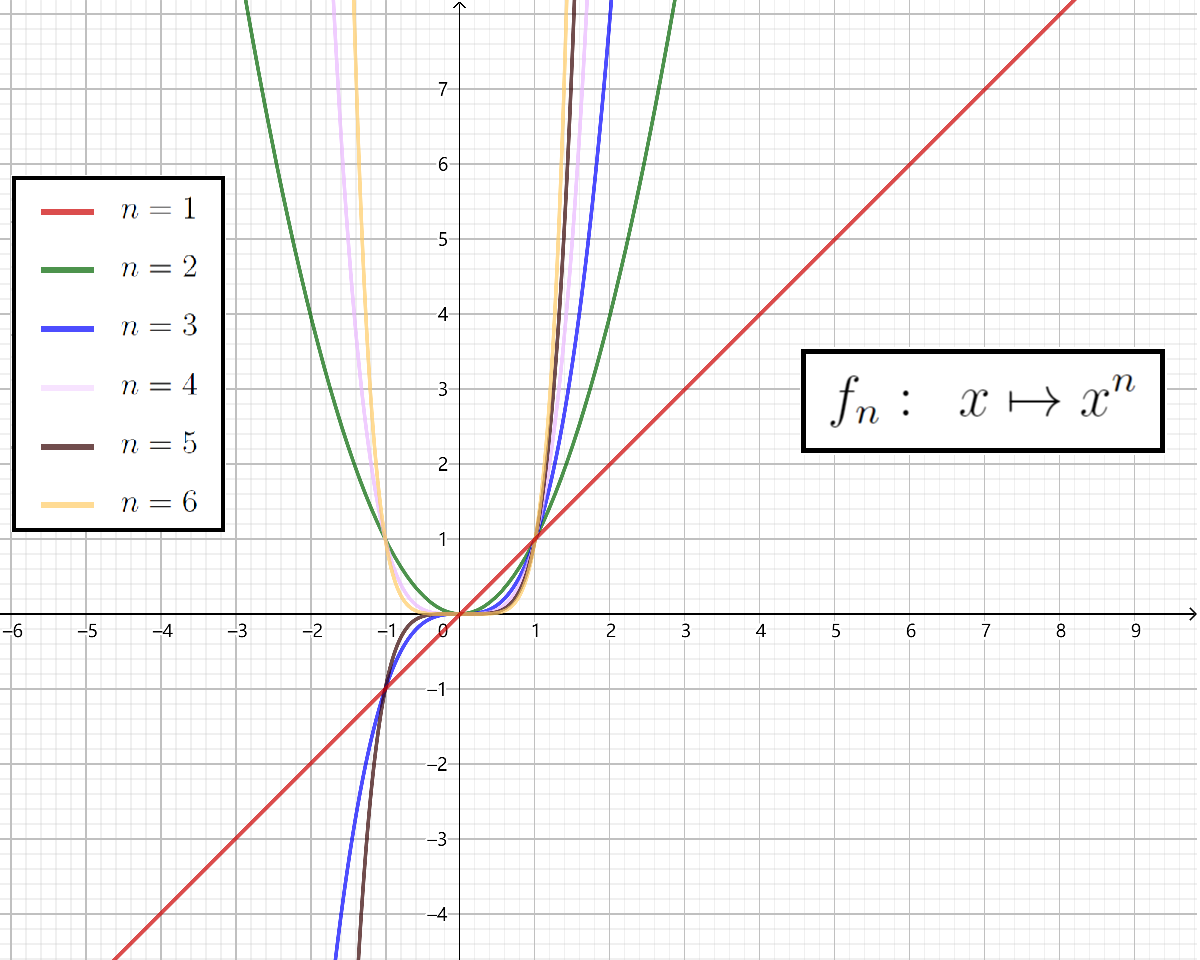
\includegraphics[width=0.8\textwidth]{整幂函数1.png}
    \caption*{\texttt{整幂函数}$x\mapsto x^n$\texttt{的图像}}
\end{figure}

从图像中可以发现,$n$是奇数的时候,函数图像关于原点对称。$n$是偶数的时候,函数图像关于$y$轴对称。
我们说具有前一种性质的函数是奇函数,具有后一种性质的函数是偶函数。
\begin{df}\textbf{实变函数的奇偶性质}
    给定实变函数$f$。如果对$f$定义域中任何$x$,都有$f(-x) = f(x)$,就说$f$是\textbf{偶函数}。
如果对$f$定义域中任何$x$,都有$f(-x) = -f(x)$,就说$f$是\textbf{奇函数}。
\end{df}

要注意的是,奇(偶)函数的定义中隐含了“函数定义域关于$0$对称”的要求。因为如果$f(-x)$没有定义,
就不存在$f(-x) = f(x)$或$f(-x) = -f(x)$的性质了。

由奇(偶)函数的定义,研究奇(偶)函数时,我们往往只需要研究半个定义域,另外一半的性质通过对称性就可以得到。

比如,研究区间$(-3, \,\,3)$上的偶函数$g$,我们只需要研究$g$在$[0, \,\,3)$上的性质。$g$在区间$(-3,\,\,0]$上的性质,可以通过
$g(-x) = -g(x)$得到。

任何奇函数$f$,如果在$0$处有定义,总有$f(0) = - f(-0) = - f(0)$,所以$f(0) = 0$。偶函数在$0$处的值则不一定是$0$。

对定义域关于$0$不对称,但在对称范围内是奇(偶)函数的函数,也可以将其自然补全。

比如,在区间$[-1,\,\,2]$上定义函数$f: x\mapsto x^2$。$f$在$[-1,\,\,1]$上是偶函数,但定义域不对称。
我们可以自然地将$f$的定义域补全到$[-2,\,\,2]$。定义在区间$[-2,\,\,2]$上的新函数$f: x\mapsto x^2$就是偶函数了。

从图像中还可以发现,$n$是偶数的时候,$f_n$总大于等于$0$。$n$是奇数的时候,
$f_n(x)$可以大于任何给定的数,也可以小于任何给定的数。如果把$f_n$的值域看作实数集的子集,
那么$n$是偶数的时候,值域有下界,$n$是奇数的时候,值域是无界的。

我们把函数值域的有界性质称为\textbf{函数的有界性质},归纳如下:
\begin{df}\textbf{实变函数的有界性质}\\
    给定实变函数$f$。
    \begin{itemize}
        \item 如果有某个数$M$,使得对$f$定义域中任何$x$,都有$f(x)\leqslant M$,就说$f$\textbf{有上界} (具体来说,有上界$M$)。
        如果不存在这样的$M$,就说$f$\textbf{无上界}。
        \item 如果有某个数$M$,使得对$f$定义域中任何$x$,都有$f(x)\geqslant M$,就说$f$\textbf{有下界} (具体来说,有下界$M$)。
        如果不存在这样的$M$,就说$f$\textbf{无下界}。
        \item 既有上界又有下界的函数称为\textbf{有界函数};既无上界又无下界的函数称为\textbf{无界函数}。
    \end{itemize}
\end{df}

此外,从图像中还可以观察到,对任何正整数$n$,$f_n(0) = 0$。$x>0$时,$f_n$总随着$x$的增大不断增大。
我们称$f_n$在$(0, \,\, +\infty)$上严格单调递增,或称$f_n$在在$(0, \,\, +\infty)$上是严格增函数。
如果$n$是奇数,那么$f_n$在$\mathbb{R}$上严格单调递增;如果$n$是偶数,$x<0$时,$f_n$总随着$x$的增大不断减小。
我们称$f_n$在$(-\infty,\,\, 0)$上严格单调递减,或称$f_n$在在$(-\infty,\,\, 0)$上是严格减函数。我们把这类性质称为函数的单调性质。
\begin{df}\textbf{实变函数的单调性质}\\
    给定实变函数$f$。
    \begin{itemize}
        \item 如果对$f$定义域中任意两个数$x_1 < x_2$,总有$f(x_1) \leqslant f(x_2)$,就说$f$在定义域上\textbf{单调递增},或者说$f$是\textbf{增函数}。
        \item 如果对$f$定义域中任意两个数$x_1 < x_2$,总有$f(x_1) \geqslant f(x_2)$,就说$f$在定义域上\textbf{单调递减},或者说$f$是\textbf{减函数}。
        \item 如果$f$定义域中任意两个数$x_1 < x_2$,总有$f(x_1) < f(x_2)$,就说$f$在定义域上\textbf{严格单调递增},或者说$f$是\textbf{严格增函数}。
        \item 如果$f$定义域中任意两个数$x_1 < x_2$,总有$f(x_1) > f(x_2)$,就说$f$在定义域上\textbf{严格单调递减},或者说$f$是\textbf{严格减函数}。   
    \end{itemize}
\end{df}

(严格)单调递增、递减函数,统称为(严格)单调函数。如果$f$在某个区间上(严格)单调,就把这个区间称为$f$的\textbf{单调区间},或者说$f$\textbf{在该区间上单调}。

用以上的定义,我们总结\textbf{整幂函数的基本性质}如下:
\begin{enumerate}
    \item $n$是奇数时,$f_n$是奇函数;$n$是偶数时,$f_n$是偶函数。因此只需研究它们在$[0, \,\, +\infty)$上的性质。
    \item 对任何正整数$n$,$f_n(0) = 0$。$f_n$在$(0, \,\, +\infty)$上严格单调递增。
    \item $n$是偶数时,$f_n$有下界,最小值是$0$,值域是$[0, \,\, +\infty)$。$n$是奇数时,$f_n$是无界函数,值域是$\mathbb{R}$。
    \item 如果$n>1$,那么$x>0$时,随着$x$增大,$f_n$增大得越来越快。
    \item 对于给定的$x$,若$x>1$,那么$n$越大,$f_n(x)$越大;若$0 < x<1$,那么$n$越大,$f_n(x)$越小。
\end{enumerate}

不同的整幂函数,乘以常数(常函数)再相加,就得到一般的整式函数。一般的整式函数可以写成:
\begin{align}
    p: \quad \mathcal{D} \subseteq \mathbb{R} &\rightarrow \mathbb{R} \notag \\
    x &\mapsto a_0 + a_1 x + \cdots + a_n x^n \notag
\end{align}
其中$\mathcal{D}$为其定义域。和整式一样,我们仍把$n$称为整式函数的次数,把$a_n$称为最高次项,等等。

一元有理式是变量$x$和数经过有限次加、减、乘、除法得到的式子,化简之后总能得到一元分式或整式。
一元分式对应的显式函数称为\textbf{分式函数}。反比例函数就是分式函数。分式函数和整式函数合称为\textbf{有理函数}。
一般的有理函数可以写成:
\begin{align}
    q: \quad \mathcal{D} \subseteq \mathbb{R} &\rightarrow \mathbb{R} \notag \\
    x &\mapsto \frac{a_0 + a_1 x + \cdots + a_n x^n}{b_0 + b_1x + \cdots + b_mx^m} \notag
\end{align}

整式函数的定义域$\mathcal{D}$可以是$\mathbb{R}$或它的任何子集。
分式函数的定义域则有一定约束。如果某个实数$c$使得作为分母的整式等于$0$:
$$ b_0 + b_1c + \cdots + b_m c^m = 0, $$
那么分式函数$q$在$c$处没有定义。我们把这样的$c$称为$q$的\textbf{奇点}\footnote{“奇”通“畸”,读音同“奇数”的“奇”。}。
分式函数的定义域不应包含奇点。

一类特殊的分式函数是形如:
$$ f_{-n} : \,\,\, x \mapsto x^{-n}$$
的函数。其中$n$是正整数。它们也是整幂函数,但对应的幂次是负整数。
它们也可以写成
$$ f_{-n} : \,\,\, x \mapsto \frac{1}{x^n}$$

显然,$0$是$f_{-n}$的奇点。它的定义域是$(-\infty,\,\, 0)\cup(0, \,\, +\infty)$(简记作$\mathbb{R}^*$)。

选择几个不同的$n$,通过描点法画出$f_{-n}$的图像。

\begin{figure}[h]
    \vspace{4pt}
    \centering
    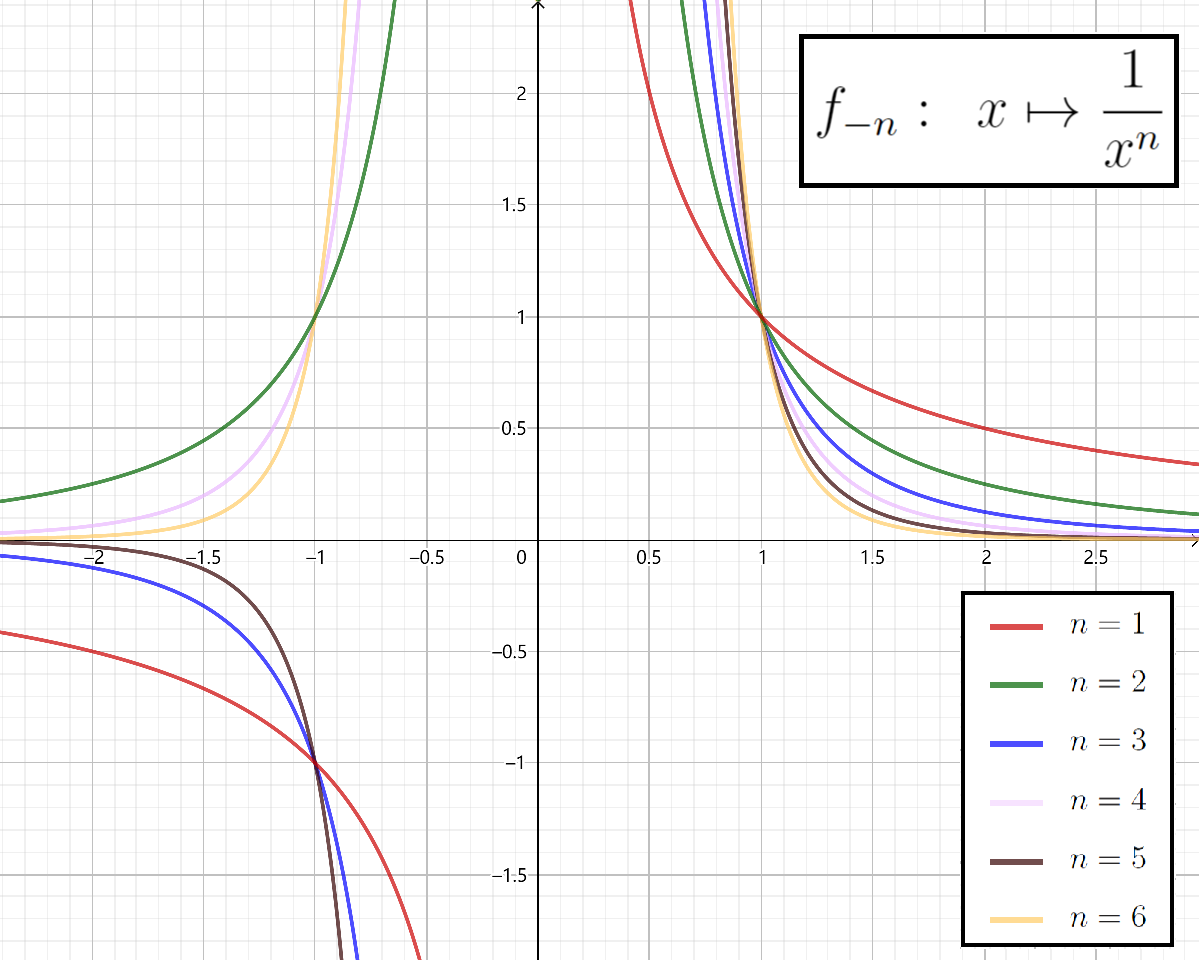
\includegraphics[width=0.8\textwidth]{整幂函数2.png}
    \caption*{\texttt{整幂函数}$x\mapsto x^{-n}$\texttt{的图像}}
\end{figure}

观察函数图像可以发现:
\begin{enumerate}
    \item $n$是奇数时,$f_{-n}$是奇函数;$n$是偶数时,$f_{-n}$是偶函数。因此只需研究它们在$(0, \,\, +\infty)$上的性质。
    \item 对任何正整数$n$,$f_{-n}$在$(0, \,\, +\infty)$上严格单调递减。
    \item $n$是偶数时,$f_{-n}$有下界,无最小值,值域是$(0, \,\, +\infty)$。$n$是奇数时,$f_{-n}$是无界函数,值域是$\mathbb{R}^*$。
    \item 如果$n>1$,那么$x>0$时,随着$x$增大,$f_{-n}$减小得越来越慢。
    \item 对于给定的$x$,若$x>1$,那么$n$越大,$f_{-n}(x)$越小;若$0 < x<1$,那么$n$越大,$f_{-n}(x)$越大。
\end{enumerate}

\begin{sk}
    \mbox{} \\
    \indent 1. 对比数列的单调性质和函数的单调性质,有哪些相同点和不同点?\\
    \indent 2. 定义\textbf{数集的有界性质}:给定数的集合$S$。如果存在数$M$使得$\forall x \in S$,$x \leqslant M$总成立,就说$S$有上界(有上界$M$);否则说$S$无上界。
    如果存在数$M$使得$\forall x \in S$,$x \geqslant M$总成立,就说$S$有下界(有下界$M$);否则说$S$无下界。
    既有上界又有下界的集合称为有界集合;既无上界又无下界的集合称为无界集合。\\
    \indent 2.1. 能否用数集的有界性质来定义实变函数的有界性质?\\
    \indent 2.2. 某个集合$S$有上界,考虑它的上界构成的集合:$S^{\text{上}}$。$S_{\text{上}}$具有怎样的性质?\\
    \indent 2.3. 考虑$S^{\text{上}}$的下界构成的集合:$S^{\text{上}}_{\text{下}}$,它具有怎样的性质?\\
    \indent 3. 是否能类比奇函数和偶函数,定义奇数列和偶数列?
\end{sk}

\section{分幂函数和无理函数}
以上的函数是关于整式和分式的。它们是$x$和数加减乘除得到的代数式。
如果再添加开方运算,我们就能得到一元无理式。当然,开方得到的式子不总是无理式,
比如$\sqrt{(x+1)^4} = (x+1)^2$就不是无理式。我们除开其中有理式的部分,
把剩余的称为无理式。

把$x$对应到一元无理式,得到的函数叫做\textbf{无理函数}。一类简单的无理函数有着和整幂函数类似的形式:
$$ f_r : \quad x \mapsto x^r. $$
其中$r$是有理数。我们称它为\textbf{分幂函数}。把$r$写成既约分数的形式。
$r > 0$时,记$r = \frac{p}{q}$,分幂函数就写成:
$$ f_r : \quad x \mapsto x^\frac{p}{q} = \sqrt[q]{x^p}. $$
$r < 0$时,记$r = -\frac{p}{q}$,分幂函数就写成:
$$ f_r : \quad x \mapsto x^{-\frac{p}{q}} = \frac{1}{\sqrt[q]{x^p}} . $$
我们不讨论$r=0$和$q=1$的情况(前者是常函数,后者是整幂函数)。

选择几个正有理数$r = \frac{p}{q} > 0$,用描点法大致画出$f_r$的图像:

\begin{figure}[h]
    \vspace{4pt}
    \centering
    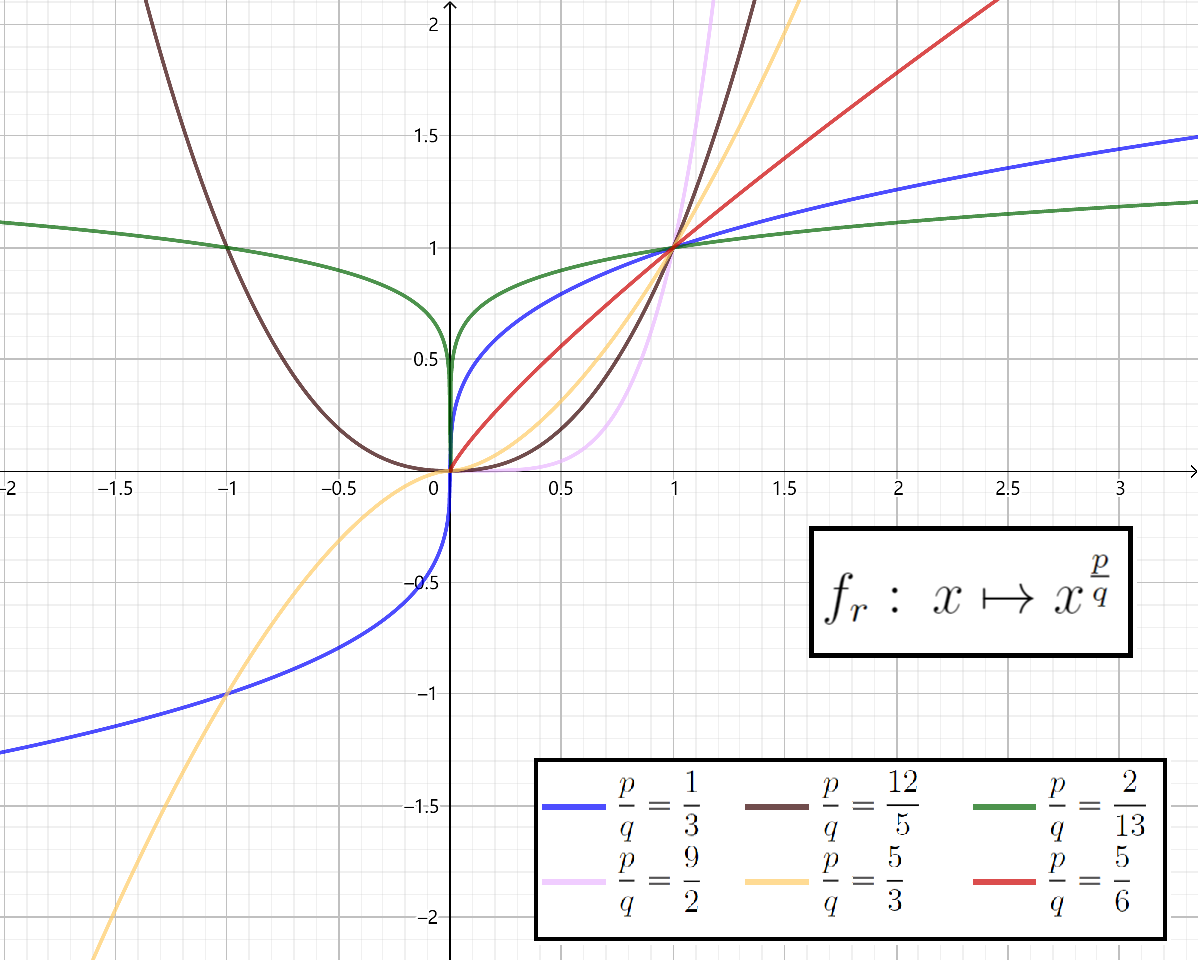
\includegraphics[width=0.8\textwidth]{分幂函数2.png}
    \caption*{\texttt{分幂函数}$x\mapsto x^\frac{p}{q}$\texttt{的图像}}
\end{figure}

观察图像可以发现:
\begin{enumerate}
    \item $p, q$是奇数时,$f_r$是奇函数;$p$是偶数$q$是奇数时,$f_r$是偶函数。因此只需研究它们在$[0, \,\, +\infty)$上的性质。
    \item $p$是奇数$q$是偶数时,$f_r$只在$[0,\,\,  +\infty)$上有定义。
    \item 对任何$r > 0$,$f_r(0) = 0$。$f_r$在$(0, \,\, +\infty)$上严格单调递增。
    \item $p, q$之一是偶数时,$f_r$有下界,最小值是$0$,值域是$[0, \,\, +\infty)$。$p, q$是奇数时,$f_r$是无界函数,值域是$\mathbb{R}$。
    \item $x>0$时,如果$r>1$,随着$x$增大,$f_r$增大得越来越快;如果$0 < r < 1$,随着$x$增大,$f_r$增大得越来越慢。
    \item 对于给定的$x$,若$x>1$,那么$r$越大,$f_r(x)$越大;若$0 < x<1$,那么$r$越大,$f_r(x)$越小。
\end{enumerate}
对比整幂函数,可以发现,除了定义域以外,大多数时候$f_r$的性质与$f_n$的性质相符。

选择几个负有理数$r = -\frac{p}{q} < 0$,用描点法大致画出$f_r$的图像:

\begin{figure}[h]
    \vspace{4pt}
    \centering
    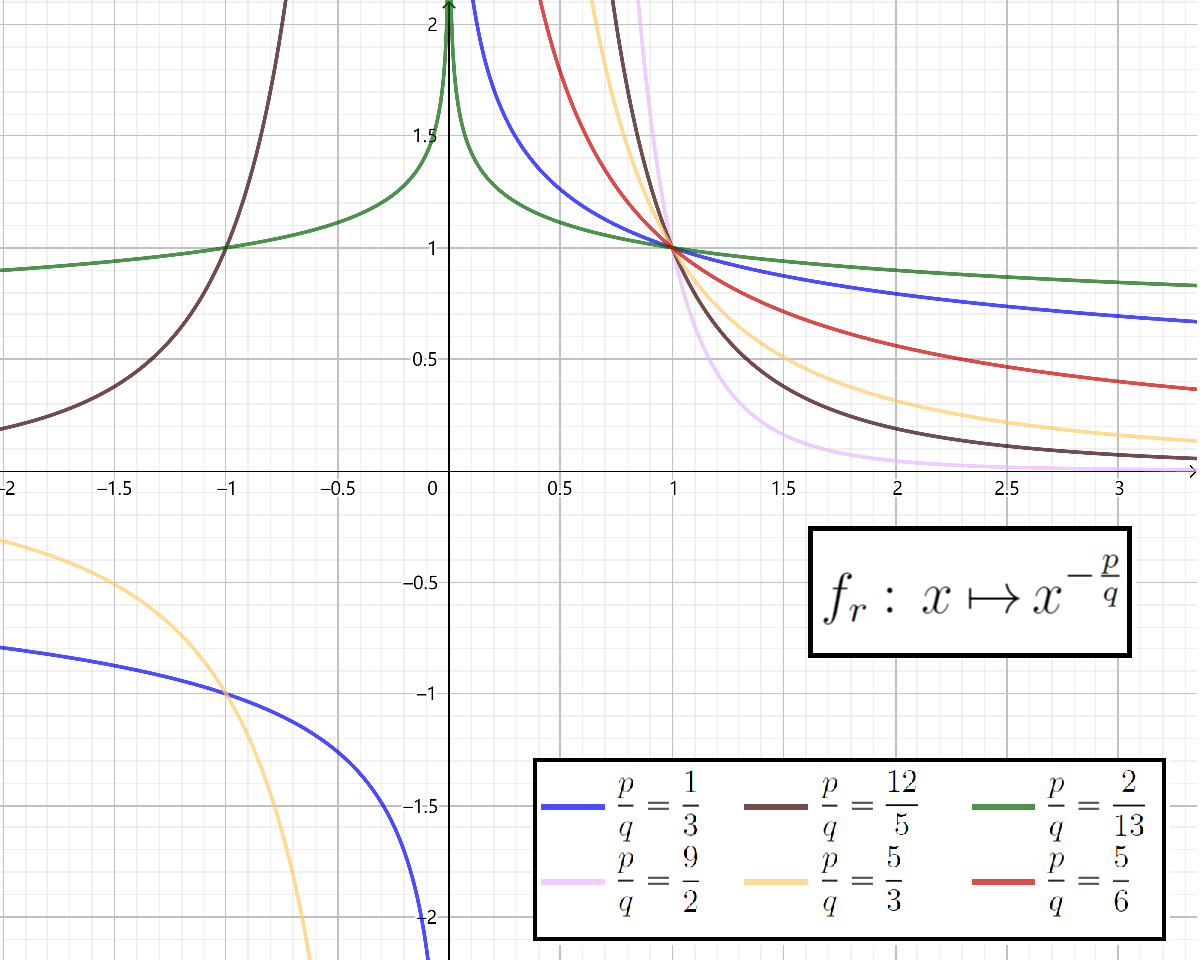
\includegraphics[width=0.8\textwidth]{分幂函数3.png}
    \caption*{\texttt{分幂函数}$x\mapsto x^{-\frac{p}{q}}$\texttt{的图像}}
\end{figure}

观察图像可以发现:
\begin{enumerate}
    \item $p, q$是奇数时,$f_r$是奇函数;$p$是偶数$q$是奇数时,$f_r$是偶函数。因此只需研究它们在$(0, \,\,  +\infty)$上的性质。
    \item $p$是奇数$q$是偶数时,$f_r$只在$(0, \,\, +\infty)$上有定义。
    \item 对任何$r < 0$,$f_r$在$(0, \,\, +\infty)$上严格单调递减。
    \item $p, q$之一是偶数时,$f_r$有下界,无最小值,值域是$(0, \,\, +\infty)$。$p, q$是奇数时,$f_r$是无界函数,值域是$\mathbb{R}^*$。
    \item $x>0$时,如果$r>1$,随着$x$增大,$f_r$增大得越来越快;如果$0 < r < 1$,随着$x$增大,$f_r$增大得越来越慢。
    \item 对于给定的$x$,若$x>1$,那么$r$越大,$f_r(x)$越小;若$0 < x<1$,那么$r$越大,$f_r(x)$越大。
\end{enumerate}
对比整幂函数,可以发现,除了定义域以外,大多数时候$f_r$的性质与$f_{-n}$的性质相符。

不讨论过于复杂的$x\leqslant 0$的情况,设定义域为$(0, \,\, +\infty)$,我们可以把整幂函数和分幂函数一起考虑,称为\textbf{幂函数}:
\begin{align}
    f_r :\quad (0, \,\, +\infty) &\rightarrow \mathbb{R} \notag \\
    x &\mapsto x^r. \notag
\end{align}
这样,我们就可以整理出整幂函数和分幂函数的共性。
\begin{enumerate}
    \item $f_r$的值域是$(0, \,\, +\infty)$
    \item $r > 0$时,$f_r$严格单调递增;$r < 0$时,$f_r$严格单调递减。
    \item $r>1$时,随着$x$增大,$f_r$增大得越来越快;$0 < r < 1$时,随着$x$增大,$f_r$增大得越来越慢。
    \item 对于给定的$x$,若$x>1$,那么$r$越大,$f_r(x)$越小;若$0 < x<1$,那么$r$越大,$f_r(x)$越大。
\end{enumerate}

除了分幂函数,我们还可以了解以下几类简单的无理函数。

$\sqrt{ax + b}$型函数。这类函数是将一次函数开方得到的。一般形式为:
$$ x\mapsto \sqrt{ax + b}.$$
其中$a, b$是常数系数。比如,$x\mapsto \sqrt{2x - 3}$就是$\sqrt{ax + b}$类函数。

$\sqrt{ax^2 + bx + c}$型函数。这类函数是将二次函数开方得到的。一般形式为:
$$ x\mapsto \sqrt{ax^2 + bx + c}.$$
其中$a, b$是常数系数。比如,$x\mapsto \sqrt{x^2 + 2x - 3}$就是$\sqrt{ax^2 + bx + c}$类函数。

$\frac{\sqrt{ax + b}}{\sqrt{cx + d}}$型函数。这类函数是两个$\sqrt{ax + b}$类函数的商。一般形式为:
$$ x\mapsto \frac{\sqrt{ax + b}}{\sqrt{cx + d}}.$$
其中$a, b$是常数系数。比如,$x\mapsto \frac{2x - 3}{\sqrt{x + 3}}$就是$\frac{\sqrt{ax + b}}{\sqrt{cx + d}}$类函数。

\begin{figure}[h]
    \vspace{4pt}
    \centering
    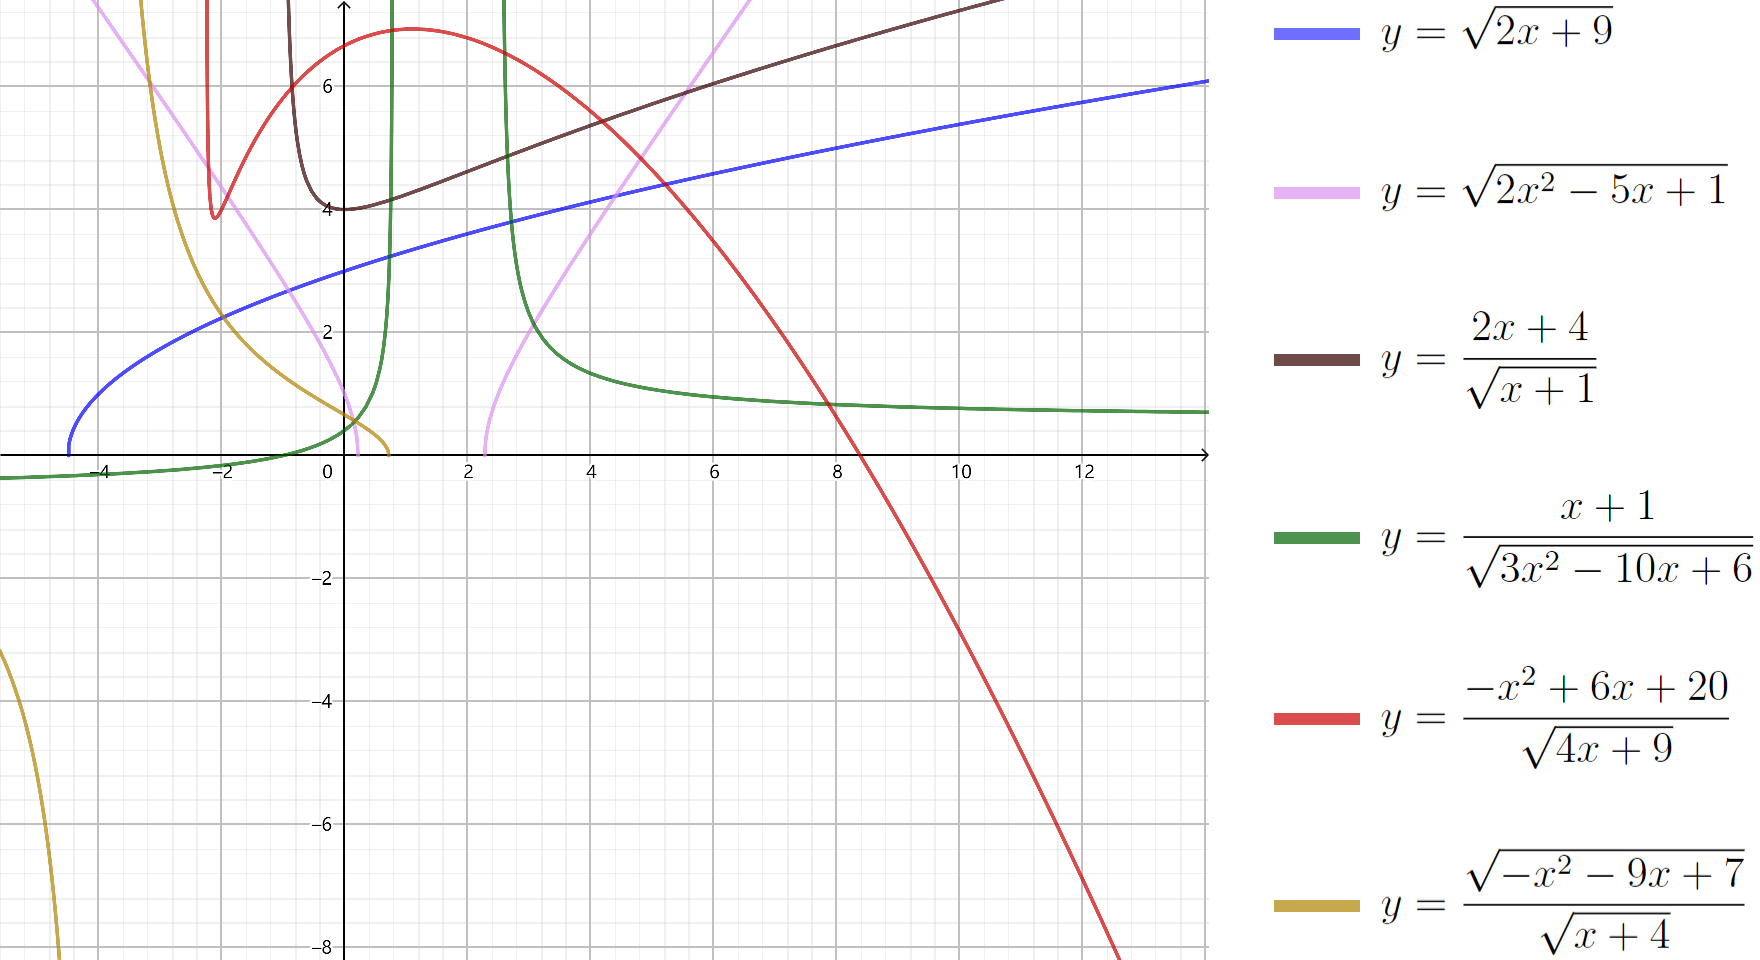
\includegraphics[width=0.96
    \textwidth]{无理函数1.png}
    \caption*{\texttt{一些无理函数的图像}}
\end{figure}

处理无理函数定义域的时候需要注意以下几点。首先,写成分式的无理函数,分母同样可能包含奇点,定义域中不包含这些奇点。
其次,偶数次开方的代数式中,根号下的值需要大于等于$0$。因此,定义域只包括使得这些值大于等于$0$的$x$。

\begin{et}
    求以下函数的定义域:\\
    \begin{align}
        (1) \,\,\quad x\mapsto \frac{\sqrt{x^2 - 3x + 2}}{x + 3} \quad & \quad (2) \quad x\mapsto \frac{\sqrt[4]{x + 1}}{\sqrt{- x^2 - 2x + 3}}\notag \\
        (3) \quad x\mapsto \frac{\sqrt{5 - 2x}}{(x - 1)\sqrt{x + 3}} \quad & \quad (4)\quad x\mapsto \frac{\sqrt{2 - x^2}}{(x^2 - 1)\sqrt{x + 0.3}} \notag 
    \end{align}
\end{et}
\begin{so}
    \mbox{}\\
    \indent 1. 这个函数包含了$\sqrt{ax^2 + bx + c}$型函数作为分子。要求根号下的值大于等于$0$,即
    $$ x^2 - 3x + 2 \geqslant 0.$$
    对左边的二次式做因式分解,得到
    $$ (x - 1)(x - 2) \geqslant 0.$$
    解集为$(-\infty, \,\, 1]\cup[2, \,\, +\infty)$。又函数分母为$x\mapsto x + 3$,有奇点$-3$。
    即$-3$不能在定义域里。于是定义域为$(-\infty,\,\,  -3)\cup(-3, \,\, 1]\cup[2,\,\,  +\infty)$。\\
    \indent 2. 这个函数的分子为偶数次开方无理函数,要求根号下的值大于等于$0$。
    另外,分母为$\sqrt{ax^2 + bx + c}$型函数,因此要求根号下的值大于$0$。于是有不等式组:
    $$\left\{\begin{array}{ccr}
        x + 1 &\geqslant 0 & \quad\quad\quad\quad (1) \\
        - x^2 - 2x + 3 &> 0  & \quad\quad\quad\quad (2)
    \end{array}\right.$$
    $(1)$的解集为$[-1,\,\, +\infty)$,$(2)$的解集为$(-3,\,\,  1)$。于是定义域为两者交集:$[-1,\,\,  1)$。\\
    \indent 3. 这个函数可以看作$\frac{\sqrt{ax + b}}{\sqrt{cx + d}}$型函数与一次函数的商。
    处理前者时,通常将分母有理化。比如这里就变为
    $$ x \mapsto \frac{\sqrt{(5 - 2x)(x + 3)}}{(x - 1)(x + 3)}. $$
    这个函数有两个奇点:$1$、$-3$。分子为偶数次开方根式,要求根号下的值大于等于$0$,即:
    $$ (5 - 2x)(x + 3) \geqslant 0$$
    解集为$[-3, \,\, 2.5]$,去掉奇点,得到定义域;$(-3, \,\, 1)\cup(1, \,\, 2.5]$。\\
    \indent 4. 这个函数涉及了$\sqrt{ax + b}$型和$\sqrt{ax^2 + bx + c}$型函数。要求分子根号下的值大于等于零,分母根号下的值大于零,并去除奇点。于是有不等式组:
    $$\left\{\begin{array}{ccr}
        2 - x^2 &\geqslant 0 & \quad\quad\quad\quad (1) \\
        x + 0.3 &> 0  & \quad\quad\quad\quad (2) \\
        x^2 - 1 &\neq 0 & \quad\quad\quad\quad (3) 
    \end{array}\right.$$
    $(1)$的解集为$[-\sqrt{2}, \,\, \sqrt{2}]$,$(2)$的解集为$(-0.3,\,\,  +\infty)$。由$(3)$知$x\neq \pm 1$。
    于是定义域为:$(-0.3, \,\, 1)\cup(1, \,\, \sqrt{2}]$。
\end{so}
\begin{sk}
    考虑无理数$s$,函数$f_s: \,\, x\mapsto x^s$是否有定义?它的定义域可以是怎样的?选几个不同的无理数$s$,按你的想法定义$f_s$,用描点法画出$f_s$大致的图像。怎样定义下的$f_s$最合理?
\end{sk}

\section{三角函数}

我们已经学习过正弦、余弦、正切、余切等三角函数。下面我们进一步整理并探讨它们的性质。

按照各种三角函数定义,我们用描点法画出它们的图像:

\begin{figure}[h] %this figure will be at the right
    \vspace{4pt}
    \centering
    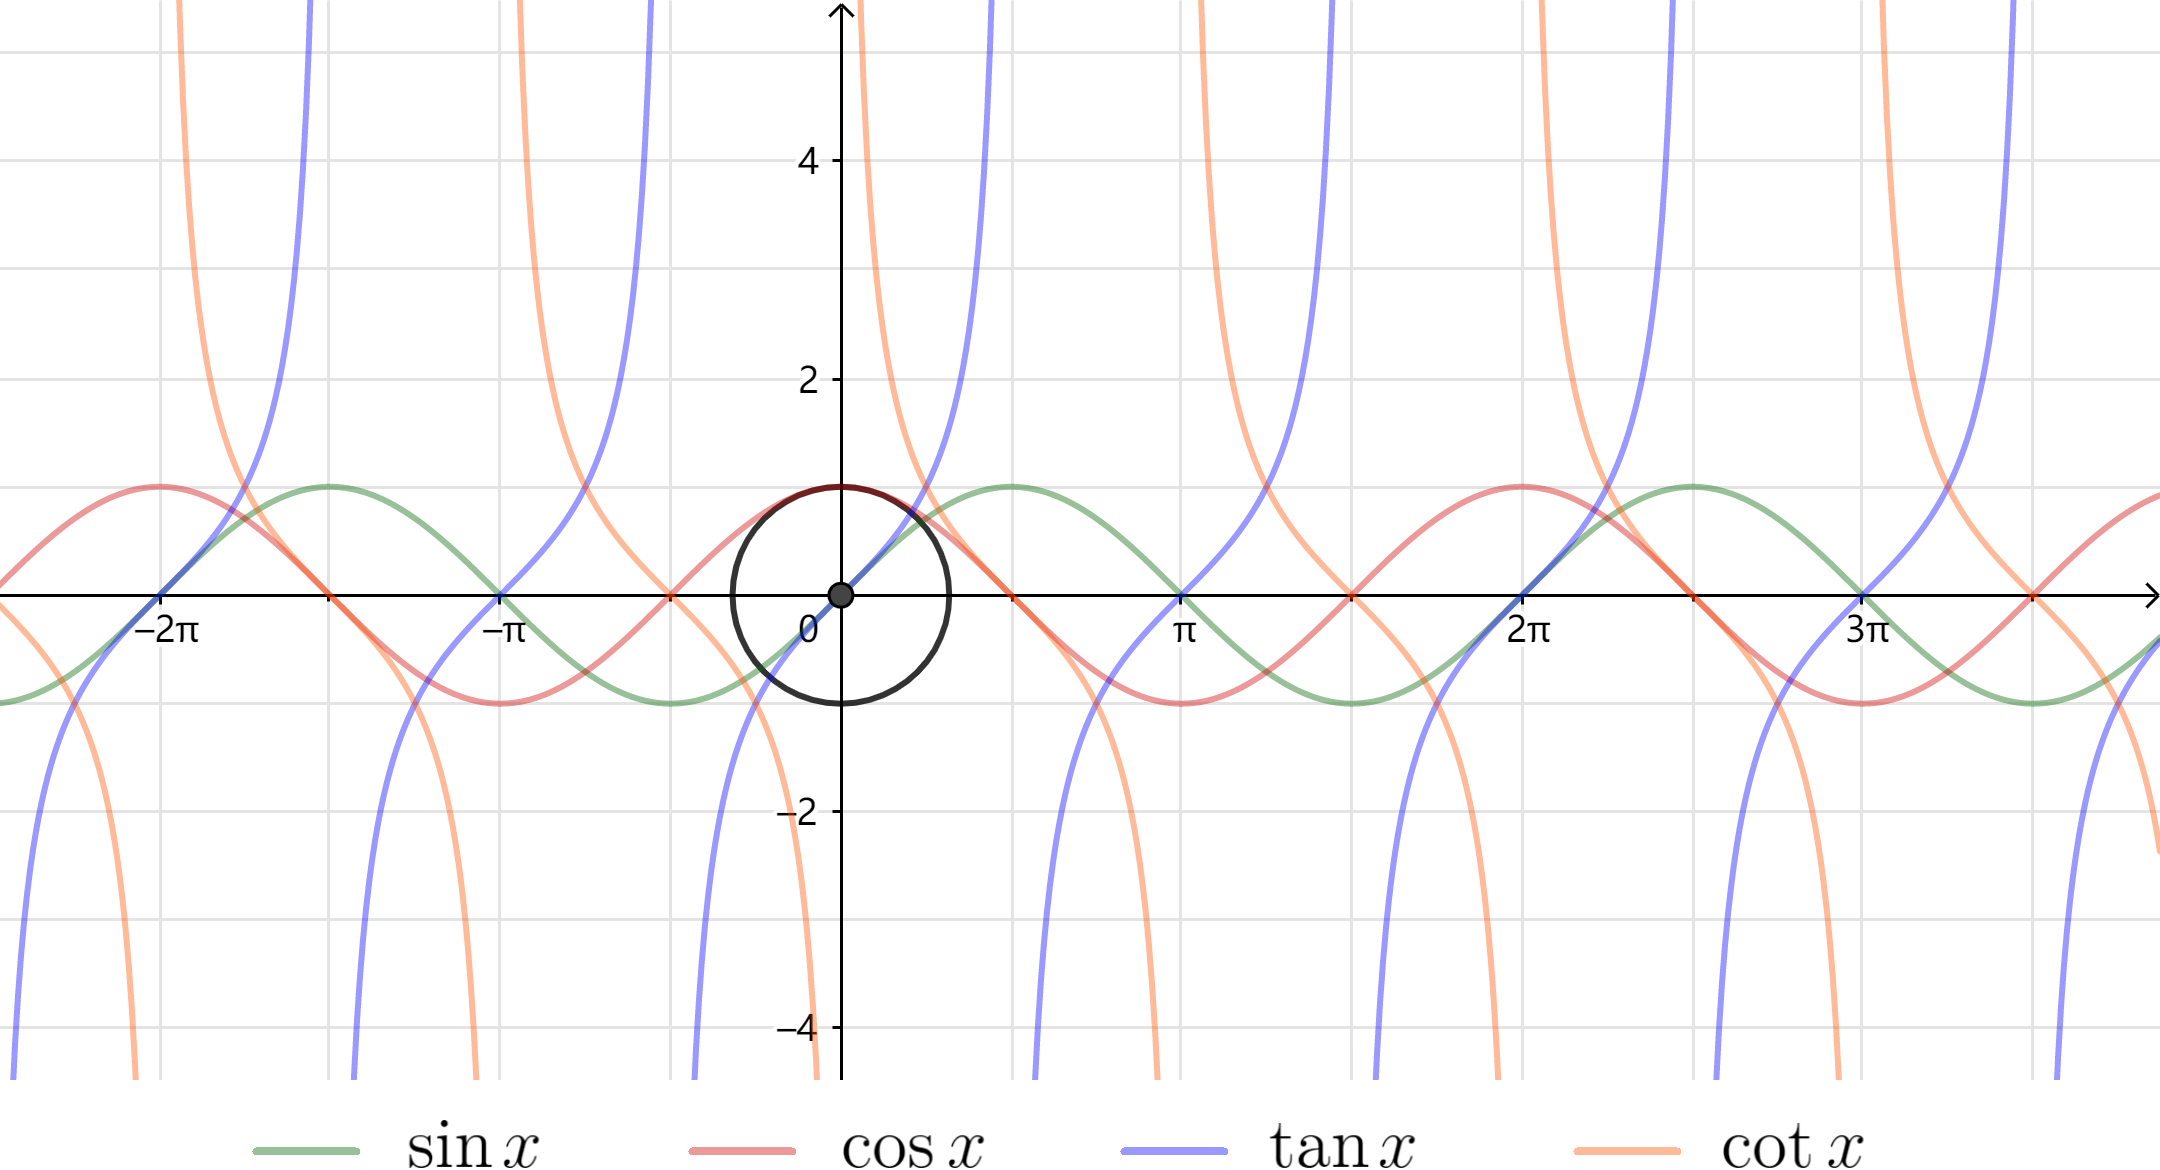
\includegraphics[width=0.96\textwidth]{三角函数1.png}
\end{figure}

这里我们使用\textbf{弧度制}代替角度制。也就是说,我们的自变量不再是角度,而是弧度,
也就是角度在单位圆中对应的圆心角的弧长。角度和弧度的转换可以用以下公式:
$$ \mbox{\texttt{弧度}} = \mbox{\texttt{角度}} \cdot \frac{\pi}{180}, \quad \mbox{\texttt{角度}} = \mbox{\texttt{弧度}} \cdot \frac{180}{\pi}. $$
比如,$30$角度对应$\frac{30\pi}{180}=\frac{\pi}{6}$弧度,
$90$角度对应$\frac{90\pi}{180}=\frac{\pi}{2}$弧度,
$1$弧度对应$\frac{180}{\pi}\approx 57.3$角度,
$\sqrt{2}$弧度对应$\frac{180\sqrt{2}}{\pi}\approx81.03$角度,等等。

从图中可以看到,正弦函数和余弦函数是有界函数,定义域是$\mathbb{R}$,值域是$[-1,1]$。
正切函数和余切函数是无界函数。正切函数的定义域是$\{x\in\mathbb{R}\,|\,x\neq (k+\frac{1}{2})\pi, \,\,\, k\in\mathbb{Z}\}$,
值域是$[-1,1]$。余切函数的定义域是$\{x\in\mathbb{R}\,|\,x\neq k\pi, \,\,\, k\in\mathbb{Z}\}$。
正弦函数和正切、余切函数是奇函数,余弦函数是偶函数。

此外,对任意实数$x$,任意整数$n$,都有$\sin(x+2n\pi) = \sin{x}$,$\cos(x+2n\pi) = \cos{x}$。
对各自定义域中任意实数$x$,任意整数$n$,都有$\tan(x+n\pi) = \tan{x}$,$\cot(x+n\pi) = \cot{x}$。
我们把这样的函数称为周期函数。
\begin{df}
    给定函数$f$。如果有某个正数$T$,使得其定义域中任何$x$,都满足
    $$ f(x + T) = f(x),$$
    就说$f$是\textbf{周期函数},$T$是$f$的\textbf{周期}。
\end{df}
注意到,如果$T$是周期函数$f$的周期,那么$2T$、$3T$、$4T$……都是$f$的周期。
$f$所有周期中若有最小的,就称它为$f$的最小周期,简称“$f$的周期是$T$”。
若不存在最小周期,就说$f$的周期为$0$。常函数是一种特殊的周期函数,任何正数$T$都是它的周期,
我们说常函数的周期是$0$。另一个例子是所谓的\textbf{示理函数}$h$,它的定义是:
$$
h(x) = \left\{
        \begin{array}{cc}
        1 & \mbox{如果}x\in\mathbb{Q} \\
        0 & \mbox{如果}x\notin\mathbb{Q} 
        \end{array}
    \right.
$$
任何有理数$r>0$都是$h$的周期:如果$x$是有理数,那么$x+r$也是有理数,于是$h(x+r) = 1 = h(x)$;
如果$x$是无理数,那么$x+r$也是无理数,于是$h(x+r) = 0 = h(x)$。

正弦和余弦函数的周期都是$2\pi$。正切和余切函数的周期都是$\pi$。

下面来研究三角函数的增减规律。由于三角函数是周期函数,只需要研究一个周期内的增减即可。
又因为三角函数总是奇函数或偶函数,其增减规律关于原点或$y$轴对称,所以只需要研究半个周期。
也就是说,对于正弦函数和余弦函数,我们只需研究区间$[0, \,\,\pi]$;对于正切函数,
只需研究区间$[0, \,\,\frac{\pi}{2})$;对于余切函数,只需研究区间$(0, \,\,\frac{\pi}{2}]$。

我们学习过正弦与余弦函数、正切与余切函数的关联。这里仅举几例:
\begin{align}
    \sin{\left(\frac{\pi}{2} - x\right)} &= \cos{x} \notag \\
    \sin{\left(x + \frac{\pi}{2}\right)} &= \cos{x} \notag \\
    \tan{\left(\frac{\pi}{2} - x\right)} &= \cot{x} \notag     
\end{align}

\begin{wrapfigure}[8]{r}{0.52\textwidth} %this figure will be at the right
    \vspace{-35pt}
    \flushright
    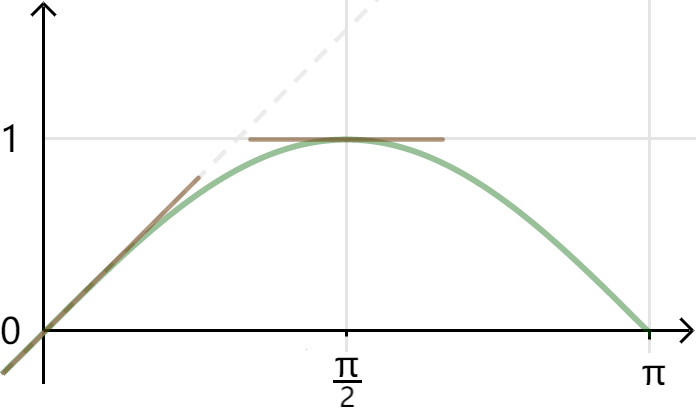
\includegraphics[width=0.5\textwidth]{三角函数2.png}
    \caption*{\texttt{正弦函数在}$[0,\,\,\pi]$\texttt{上的图像}}
\end{wrapfigure}

这些关联关系可以让我们在不同的三角函数之间转换,从不同的角度看待问题。
比如,根据第二个公式,正弦函数在区间$[0, \,\,\pi]$上的图像和余弦函数在$[-\frac{\pi}{2}, \,\,\frac{\pi}{2}]$
上的图像是一样的。根据第三个公式,正切函数和余切函数关于直线$x = \frac{\pi}{4}$对称。

现在来看正弦函数在区间$[0, \,\,\pi]$上的图像。

可以看到,正弦函数的图像总在直线$y = x$下方。在$x = 0$附近,函数值$\sin(x)\approx x$,但随着$x$增大,
$x$的正弦值增大得比$y=x$慢,到了$x=\frac{\pi}{2}$时不再继续增大,而逐渐减小,最终在$x=\pi$时再次变成$0$。

正弦函数是奇函数,所以区间$[-\pi, \,\,0]$上的函数图像与$[0, \,\,\pi]$上的图像关于原点对称。
查看整个周期$[-\pi, \,\,\pi]$,正弦函数在$[-\pi, \,\,-\frac{\pi}{2}]$上严格单调递减;
然后在$[-\frac{\pi}{2}, \,\,\frac{\pi}{2}]$上严格单调递增,又在$[\frac{\pi}{2}, \,\,\pi]$上严格单调递减。
用变化表可以概括为:

\begin{figure}[h] %this figure will be at the right
    % \vspace{-4pt}
    \centering
    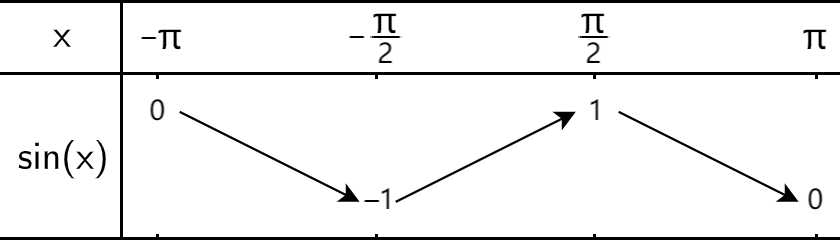
\includegraphics[width=0.63\textwidth]{三角函数变化表1.png}
\end{figure}

余弦函数的增减规律和正弦函数几乎一样。发生在正弦函数$x=x_0$处的事情,
在余弦函数$x=x_0-\frac{\pi}{2}$处发生。因此,在周期区间$[-\pi, \,\, \pi]$上,
余弦函数的增减规律可以用以下变化表概括:

\begin{figure}[h] %this figure will be at the right
    % \vspace{-4pt}
    \centering
    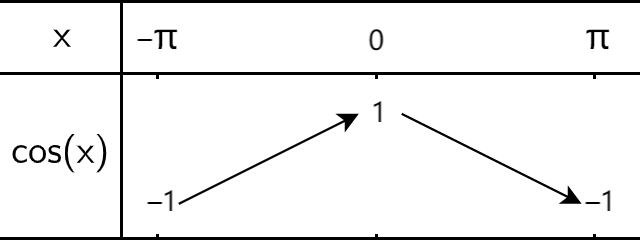
\includegraphics[width=0.48\textwidth]{三角函数变化表2.png}
\end{figure}

正切函数在单个周期内严格单调递增,但在整个定义域中并不是单调函数。
同样,余切函数在单个周期内严格单调递减,但在整个定义域中并不是单调函数。

\section{复合函数和反函数}

设有映射$f$将出发集$A$中元素逐个对应到到达集$B$中元素,又有映射$g$将$f$在$B$中的目标再次对应到集合$C$中元素,
那么我们可以定义两者的\textbf{复合}:
\begin{align}
    g\circ f : \,\,\, A &\rightarrow C \notag \\
    x &\mapsto g(f(x)) \notag
\end{align}

如果$A$、$B$、$C$都是数集,我们就说函数$f$和$g$复合成为$g\circ f$。
要使得映射的复合有意义,$f$的值域$\mathcal{V}_f$应该是$g$的定义域$\mathcal{D}_g$的子集。
这样我们才能把$f(x)$对应到$C$中。如果$\mathcal{V}_f$超出了$\mathcal{D}_g$的范围,
那么我们可以“缩小”$f$的定义域$\mathcal{D}_f$,即找到$\mathcal{D}_f$的子集$\mathcal{D}'$,
使得$f(\mathcal{D}')\subseteq \mathcal{D}_g$。

要注意的是,出于书写习惯,不少人会把这个复合映射写成$f\circ g$,因为在我们的认知中,
$A$中元素先经过$f$映射到$B$中,再经过$g$映射到$C$中。不过我们书写函数的时候,自变量在函数符号的右侧,
因此,为了和$g(f(x))$的书写顺序一致,我们把这个复合映射记作$g\circ f$而不是$f\circ g$。

设函数$f:x\mapsto \sqrt{x}$,$g:x\mapsto 2x - 1$。
则复合函数$g\circ f$为$x\mapsto g(f(x)) = 2\sqrt{x} - 1$。
注意到$f$的定义域是$[0, \,\,+\infty)$,值域是$[0, +\infty)$,$g$的定义域是$\mathbb{R}$,
$g\circ f$的定义域是$[0,\,\, +\infty)$。

另一方面,复合函数$f\circ g$为$x\mapsto \sqrt{2x - 1}$。由于$g$的定义域和值域都是$\mathbb{R}$,
而$f$的定义域是$[0,\,\, +\infty)$,我们需要缩小$g$的定义域,使得$g$的值域落在$f$的定义域中。
也就是说,我们把$g$的定义域缩小到集合:$\{x \,|\, 2x - 1 \in [0, \,\,+\infty)\}$。
这个集合可以化简成$[0.5, \,\,+\infty)$。因此复合函数$f\circ g$为:
\begin{align}
    f\circ g : \,\,\, [0.5,\,\, +\infty) &\rightarrow [0,\,\, +\infty) \notag \\
    x &\mapsto \sqrt{2x - 1} \notag
\end{align}

\begin{figure}[h] %this figure will be at the right
    % \vspace{4pt}
    \centering
    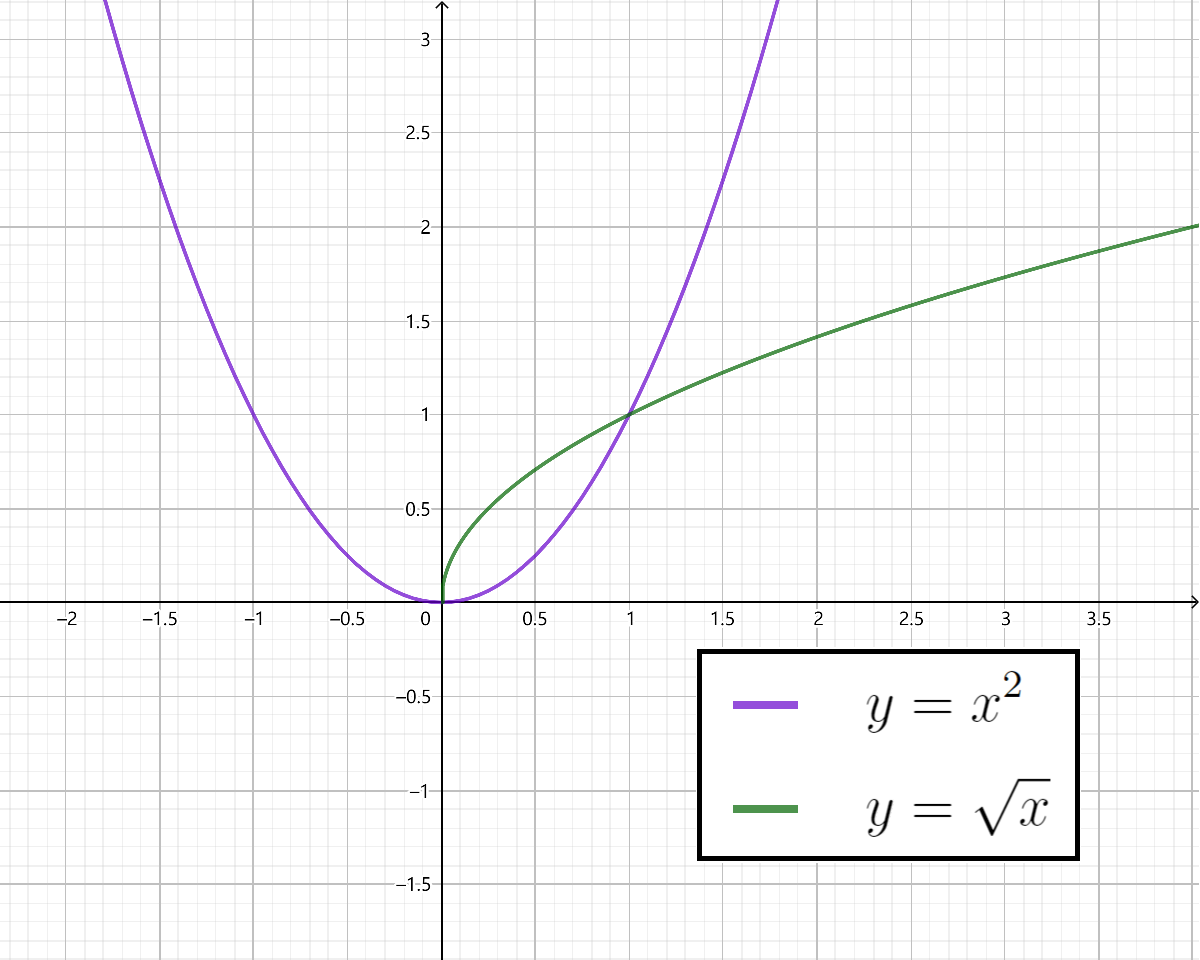
\includegraphics[width=0.64\textwidth]{反函数1.png}
    \caption*{\texttt{函数}$x\mapsto x^2$\texttt{与}$x\mapsto \sqrt{x}$}
\end{figure}

一般情况下,$g\circ f \neq f\circ g$。甚至,大多数时候,我们无法比较两者,
因为$f$的出发集$g$的到达集不同。只有当$C$和$A$“重合”的时候,我们才有可能比较$g\circ f$和$f\circ g$。

一种特殊情况是$g\circ f$为恒等映射,即对$f$的定义域$\mathcal{D}_f$中的任何元素$x$,总有$g(f(x)) = x$。
我们说这样的$g$是$f$的左逆映射。$f$把某个元素$x$对应到目标函数$y$,而$g$把$f$的目标元素$y$“逆转”为原来的$x$。

要使得$f$的左逆映射$g$有定义,我们要求$f$的定义域$\mathcal{D}_f$等于$g$的值域$\mathcal{V}_g$,
$g$的定义域$\mathcal{V}_g$包含$f$的值域$\mathcal{V}_f$。
且对任意$\mathcal{D}_f$中元素$a \neq b$,$f(a) \neq f(b)$。可以想象,如果有$a \neq b$使得$f(a) = f(b)$,
那么$a = g(f(a)) = g(f(b)) = b$,自相矛盾!我们把满足这个条件的$f$称为\textbf{单射}。

举例来说,函数$f: \,\,x \mapsto \sqrt{x}$是单射,它的定义域是非负实数集合。
可以验证,定义在全体实数上的函数$g:\,\, x \mapsto x^2$是它的左逆映射:
$$ \forall \,\, x \geqslant 0, \,\,\, g(f(x)) = \left(\sqrt{x}\right)^2 = x$$
但$f$不是$g$的左逆映射:$f(g(-1)) = 1$。不过,如果把$g$的定义域缩减到非负实数集合,那么$f$就是$g$的左逆映射了。

类似地,如果$f\circ g$是恒等映射,就说$g$是$f$的右逆映射。这时$f$的值域$\mathcal{V}_f$应当等于$g$的定义域$\mathcal{D}_g$。
我们说$f$是$\mathcal{D}_g$上的\textbf{满射}。

按照定义,$g$是$f$的左逆映射,说明$f$是$g$的右逆映射;$g$是$f$的右逆映射,说明$f$是$g$的左逆映射。

如果$g\circ f$是恒等映射,$f\circ g$也是恒等映射,就说$f$和$g$互为逆映射。如果$f$和$g$都是函数,就说它们互为\textbf{反函数}。
这时$f$和$g$既是单射也是满射。
我们把既是单射又是满射的映射称为\textbf{双射}或\textbf{一一对应}。

举例来说,$f: \,\,x\in[0,\,\,+\infty) \mapsto x^2 - 1$是双射。
它的值域是$[-1,\,\,+\infty)$对某个$x\geqslant 0$,记$y = f(x) = x^2 - 1$,
于是$x = \sqrt{y + 1}$。定义函数$g:x\in[-1, \,\,\infty)\mapsto\sqrt{x + 1}$。
那么$\forall x \geqslant 0$,$g(f(x)) = \sqrt{x^2 - 1 + 1} = x$,
$f(g(x)) = \left(\sqrt{x + 1}\right)^2 - 1 = x$。于是$f$和$g$互为反函数。

\begin{figure}[h] %this figure will be at the right
    \vspace{4pt}
    \centering
    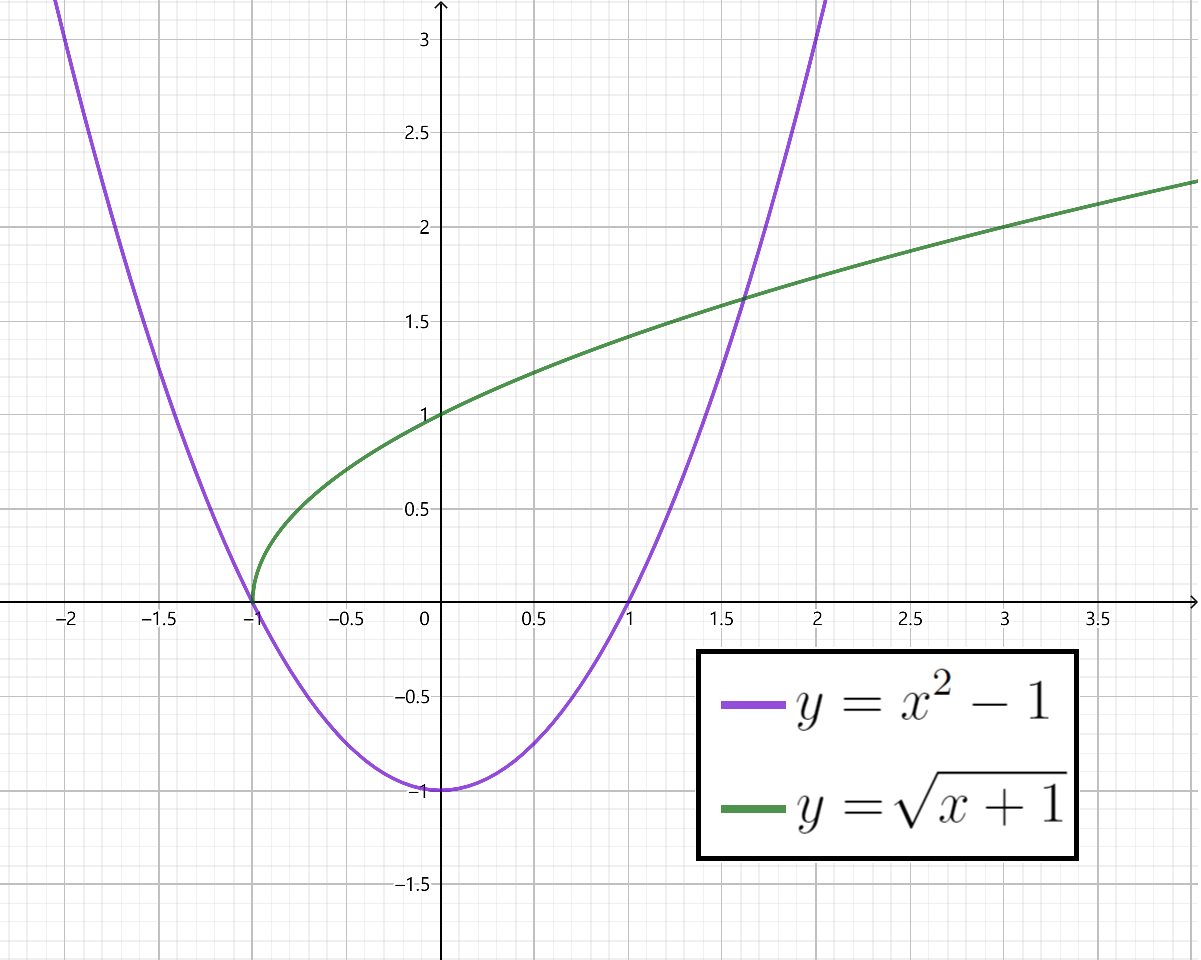
\includegraphics[width=0.64\textwidth]{反函数2.png}
    \caption*{\texttt{函数}$x\mapsto x^2 - 1$\texttt{与}$x\mapsto \sqrt{x + 1}$}
\end{figure}

反函数和本函数有什么联系?我们来看它们在平面直角坐标系中的图像。
设$(x, y)$是$f$的图像上一点,则$y = f(x)$,因此$g(y) = x$。
这说明$(y, x)$是$g$的图像上一点。反过来,如果$(x,y)$是$g$的图像上一点,
则$y = g(x)$,因此$f(y) = x$。这说明$(y, x)$是$f$的图像上一点。
简而言之,交换函数图像上一点的横坐标和纵坐标,就得到它的反函数的图像上一点的坐标。

比如,我们用描点法画出$f: x\in[0,\,\,+\infty) \mapsto x^2 - 1$的图像,
交换每个点的横坐标和纵坐标,得到的新坐标可以描出函数$g:x\in[-1, \,\,\infty)\mapsto\sqrt{x + 1}$的图像。
如果我们作直线$l: y = x$,会发现$f$和$g$的图像关于直线$l$对称。这不难证明:

设$P(a,b)$为$f$图像上一点,则$Q(b,a)$为$g$图像上一点。
过两点的直线为$l':x + y = a + b$。$l'$与$l$垂直,
相交于点$M(\frac{a+b}{2}, \frac{a+b}{2})$,而$|PM| = \frac{|a-b|}{\sqrt{2}} = |QM|$,
因此$l$是$P,Q$中垂线,$P,Q$关于$l$对称。从$g$图像上一点出发,结论相同。这就说明两者图像关于$l$对称。

这种对称性告诉我们,函数的反函数如果存在,应该是唯一的。下面来证明这一点:

\begin{tm}[逆映射的唯一性]
    逆映射如果存在则唯一。
\end{tm}
\begin{proof}
    设$g_1$、$g_2$是$f$的逆映射,则它们既是$f$的左逆映射,也是它的右逆映射。因此,对于$f$值域中任何元素$y$,
    有唯一的$x$使得$y = f(x)$,
    $$ g_1(y) = g_1(f(x)) = x = g_2(f(x)) = g_2(y).$$
    $f$的值域就是$g_1$、$g_2$的定义域。因此,$g_1$、$g_2$相等。
\end{proof}

\begin{et}\label{et:1-3-0}
    求以下函数的反函数:\\
    \indent 1. $f:\,\,\,x \mapsto x^r$\\
    \indent 2. $f:\,\,\,x \mapsto \frac{1}{x + 1}$\\
    \indent 3. $f:\,\,\,x \mapsto \sqrt{1 - x^2}$
\end{et}
\begin{so}
    \mbox{} \\
    根据反函数的唯一性,我们只需找到$f$的一个反函数。

    \indent 1. 首先来看$r$为正整数的情况。$r$为奇数时,$f$在$\mathbb{R}$上为单射。
    $r$为偶数时,$f$在$\mathbb{R}$上不为单射,我们只考虑区间$[0, +\infty)$。按照幂函数的定义,
    在我们考虑的范围内,$g: x\mapsto x^{\frac{1}{r}}$使得
    \begin{align}
        \forall x, \,\,\, g(f(x)) &= \left(x^r\right)^{\frac{1}{r}} = x \notag \\
        \forall x, \,\,\, f(g(x)) &= \left(x^{\frac{1}{r}}\right)^{r} = x \notag 
    \end{align} 
    因此,$g$是$f$的反函数。\\  
    再来看$r$为有理数的情况。设$r = \frac{p}{q}$,其中$p,q$为互素的整数。$f$在区间$[0,\,\,\infty)$上严格单调,
    因此我们只考虑$[0,\,\,\infty)$。\\
    $\frac{1}{r} = \frac{q}{p}$。对任何正数$x$,
    \begin{align}
        \left(x^r\right)^{\frac{1}{r}} &= \left(x^{\frac{p}{q}}\right)^{\frac{q}{p}} = \left(\left(\left(x^{p}\right)^\frac{1}{q}\right)^q\right)^\frac{1}{p} \notag \\
                                       &= \left(x^{p}\right)^\frac{1}{p} = x \notag
    \end{align}
    \begin{align}
        \left(x^{\frac{1}{r}}\right)^r &= \left(x^{\frac{q}{p}}\right)^{\frac{p}{q}} = \left(\left(\left(x^{q}\right)^\frac{1}{p}\right)^p\right)^\frac{1}{q} \notag \\
                                       &= \left(x^{q}\right)^\frac{1}{q} = x \notag
    \end{align}
    因此,$f$的反函数是$x\mapsto x^{\frac{1}{r}}$。\\
    \indent 2. $f$在其定义域内是单射,因此,我们可以放心地寻找它的反函数。
    设$y = f(x) = \frac{1}{x+1}$,则$x = \frac{1 - y}{y}$。因此,考虑函数$g: x\mapsto \frac{1 - x}{x}$。
    在我们考虑的范围内,
    \begin{align}
        \forall x\neq 1, \,\,\, g(f(x)) &= g\left(\frac{1}{x+1}\right) \notag \\
                                  &= \frac{1 - \frac{1}{1 + x}}{\frac{1}{x + 1}} \notag \\
                                  &= \frac{x + 1 - 1}{1} = x. \notag
    \end{align} 
    同理,
    \begin{align}
        \forall x \neq 0, \,\,\, f(g(x)) &= f\left(\frac{1 - x}{x}\right) \notag \\
                                  &= \frac{1}{\frac{1 - x}{x} + 1} \notag \\
                                  &= \frac{x}{1 - x + x} = x. \notag
    \end{align} 
    这说明,$g$是$f$的反函数。\\  
    \indent 3. $f$在其定义域内不是单射,我们只考虑区间$[0,1]$。
    设$y = \sqrt{1 - x^2}$,则$x^2 + y^2 = 1$,因此,$x = \sqrt{1 - y^2}$。这说明,我们要找的函数很可能就是$f$自己。
    下面来验证这一点:
    \begin{align}
        \forall x\in [0,\,\,1], \,\,\, f(f(x)) &= f\left(\sqrt{1 - x^2}\right) \notag \\
                                  &= \sqrt{1 - \left(\sqrt{1 - x^2}\right)^2} \notag \\
                                  &= \sqrt{1 - 1 + x^2} = x. \notag
    \end{align} 
    因此,$f$的反函数是它自己。
\end{so}

\begin{sk}
    如果$g$是$f$的左逆映射,并且$g$的定义域$\mathcal{V}_g$等于$f$的值域$\mathcal{V}_f$,能否说明$f$是$g$的左逆映射?为什么?
\end{sk}
\begin{xt}
    \mbox{} \\
    \indent 1. 画出习题\ref{et:1-3-0}中各个函数和反函数的图像。\\
    \indent 2. 求以下函数的反函数:\\
    \indent 2.1. $x\mapsto $
\end{xt}

\section{反三角函数}

下面来看三角函数的反函数。三角函数是周期函数,所有三角函数$f$都满足$f(x+2\pi) = f(x)$,因此不是单射。
我们退而求其次,只考虑三角函数在部分定义域上的反函数。从上一节可知,反函数的图像和本函数的图像关于直线$l: y = x$对称。
因此,画出三角函数的函数图像后,我们就可以直观地了解反三角函数的图像。

\begin{figure}[h] %this figure will be at the right
    \vspace{4pt}
    \centering
    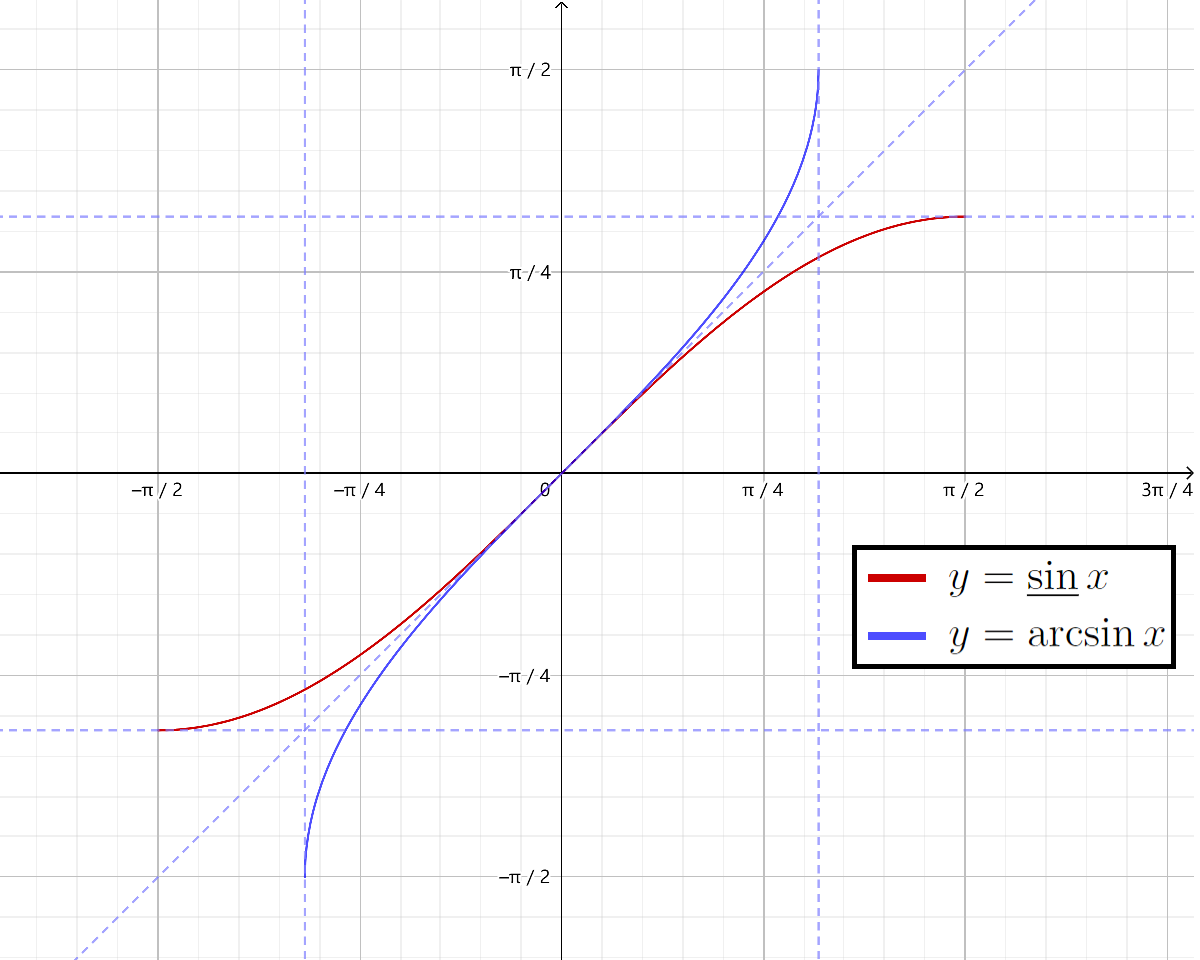
\includegraphics[width=0.8\textwidth]{反正弦函数1.png}
    \caption*{\texttt{反正弦函数}$x\mapsto \arcsin(x)$}
\end{figure}

首先来看正弦函数($\sin$)的反函数。我们希望选择一个最长的区间,让正弦函数在这个区间上是单射。
常用的区间是$[-\frac{\pi}{2}, \,\, \frac{\pi}{2}]$。
正弦函数在$[-\frac{\pi}{2}, \,\, \frac{\pi}{2}]$上严格单调递增,从$-1$增长到$1$。我们把正弦函数在这个区间上的部分记作$\underline{\sin}$:
\begin{align}
     \underline{\sin} : [-\frac{\pi}{2}, \,\, \frac{\pi}{2}] &\rightarrow [-1,\,\, 1]\notag \\
                                                           x &\mapsto \sin{x} \notag
\end{align}
画出它的图像,按照直线$l: y = x$作对称,就得到它的反函数,称为\textbf{反正弦函数},记作$\arcsin$:
$$ \arcsin : [-1,\,\, 1] \rightarrow [-\frac{\pi}{2}, \,\, \frac{\pi}{2}] . $$
$\arcsin$中的“arc”是“弧长”的意思。$\arcsin$最初表示“把$[-1,\,\, 1]$中的数按正弦函数的反函数对应到单位圆上的弧长”。

举例来说,$\arcsin{1} = \frac{\pi}{2}$,$\arcsin{(-1)} = -\frac{\pi}{2}$,
$\arcsin{0.5} = \frac{\pi}{6}$,$\arcsin{\frac{\sqrt{3}}{2}} = \frac{\pi}{3}$,等等。

从图像中可以看出,反正弦函数也是严格单调递增的函数。它的定义域是$[-1,\,\, 1]$、值域是$[-\frac{\pi}{2}, \,\, \frac{\pi}{2}]$。
$\underline{\sin}$是奇函数,因此,反正弦函数也是奇函数。$x > 0$时,反正弦函数
总在直线$l$上方,增长越来越快;
$x < 0$时,反正弦函数总在直线$l$下方,增长越来越慢。

反正弦函数的定义域是正弦函数的值域。因此,$\sin{(\arcsin{x})} = x$对$[-1,\,\, 1]$中的数总成立。
但反正弦函数的值域只是正弦函数的定义域的真子集,因此,$\arcsin{(\sin{x})} = x$只对$[-\frac{\pi}{2}, \,\, \frac{\pi}{2}]$中的数成立。

再来看余弦函数的反函数。由$\cos{x} = \sin(x+\frac{\pi}{2})$可知,余弦函数的图像可以看作正弦函数的图像按向量$\left(-\frac{\pi}{2}, 0\right)$
平移的结果。因此,我们可以选择$[-\pi, \,\, 0]$作为研究区间。由于余弦函数是偶函数,我们也可以选择$[0,\,\,\pi]$作为研究区间。
常用的区间是$[0,\,\,\pi]$。余弦函数在$[0,\,\,\pi]$上严格单调递减,从$1$减少到$-1$。我们把余弦函数在这个区间上的部分记作$\underline{\cos}$:
\begin{align}
    \underline{\cos} : [0,\,\,\pi] &\rightarrow [-1,\,\, 1]\notag \\                                  x &\mapsto \cos{x} \notag
\end{align}
画出它的图像,按照直线$l: y = x$作对称,就得到它的反函数,称为\textbf{反余弦函数},记作$\arccos$:
$$ \arccos : [-1,\,\, 1] \rightarrow [0,\,\,\pi] . $$

\begin{figure}[h] %this figure will be at the right
    \vspace{4pt}
    \centering
    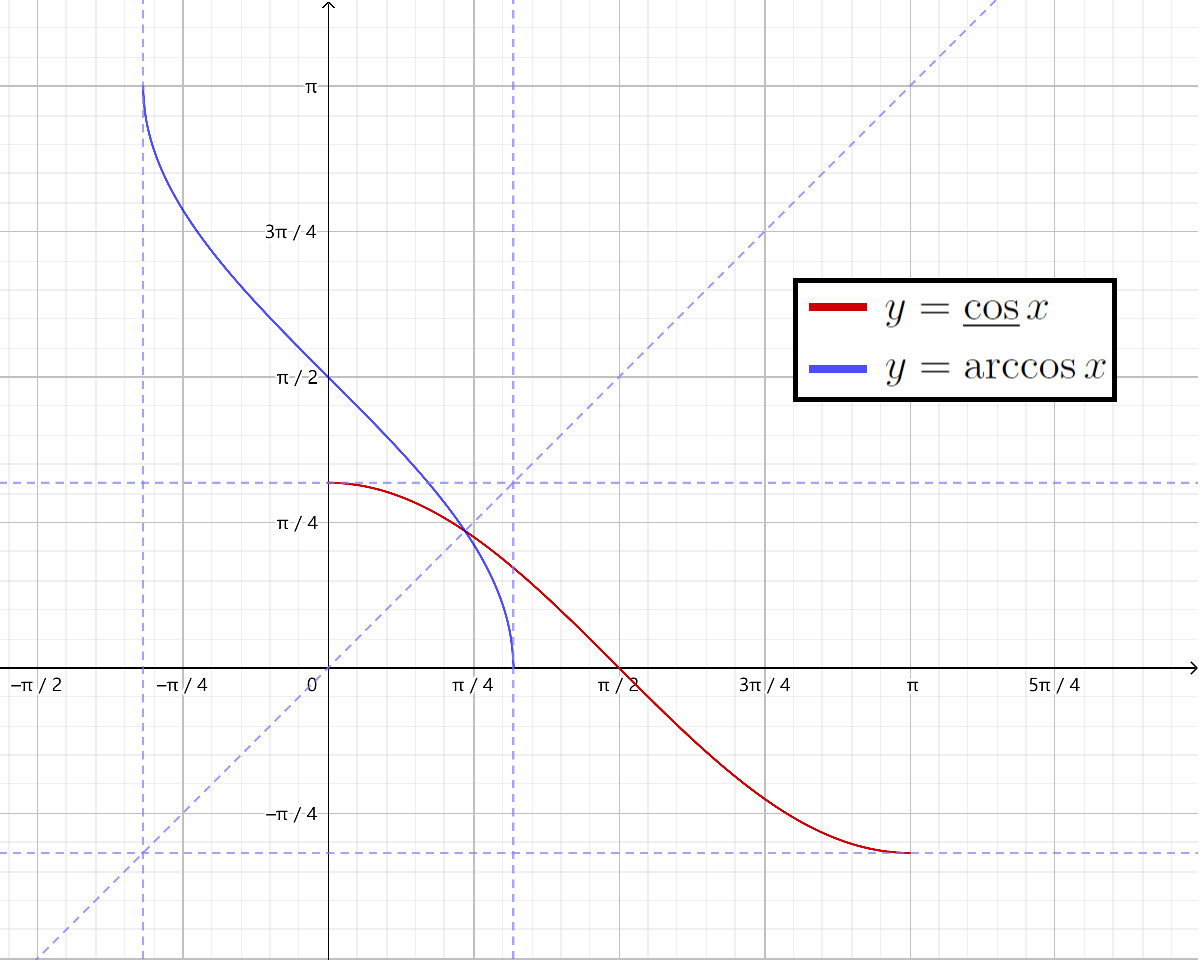
\includegraphics[width=0.8\textwidth]{反余弦函数1.png}
    \caption*{\texttt{反余弦函数}$x\mapsto \arccos(x)$}
\end{figure}

从图像中可以看出,反余弦函数也是严格单调递减的函数。它的定义域是$[-1,\,\, 1]$、值域是$[-\frac{\pi}{2}, \,\, \frac{\pi}{2}]$。
$x < 0$时,反余弦函数总大于$\frac{\pi}{2}$,减少得越来越慢;$x > 0$时,反余弦函数总小于$\frac{\pi}{2}$,减少得越来越快。

举例来说,$\arccos{1} = 0$,$\arccos{0} = \frac{\pi}{2}$,
$\arccos{(-1)} = \pi$,$\arccos{0.5} = \frac{\pi}{3}$,$\arccos{\frac{\sqrt{3}}{2}} = \frac{\pi}{6}$,等等。

反余弦函数的定义域是余弦函数的值域。因此,$\cos{(\arccos{x})} = x$对$[-1,\,\, 1]$中的数总成立。
但反余弦函数的值域只是余弦函数的定义域的真子集,因此,$\arccos{(\cos{x})} = x$只对$[0,\,\,\pi]$中的数成立。

接下来看正切函数的反函数。正切函数的最小正周期是$\pi$,在$(-\frac{\pi}{2}, \,\, \frac{\pi}{2})$上严格单调递增。
我们把正切函数在这个区间上的部分记作$\underline{\tan}$:
\begin{align}
    \underline{\tan} : (-\frac{\pi}{2}, \,\, \frac{\pi}{2}) &\rightarrow \mathbb{R} \notag \\
                                                          x &\mapsto \tan{x} \notag
\end{align}
画出它的图像,按照直线$l: y = x$作对称,就得到它的反函数,称为\textbf{反正切函数},记作$\arctan$:
$$ \arctan : \mathbb{R} \rightarrow (-\frac{\pi}{2}, \,\, \frac{\pi}{2}) . $$

\begin{figure}[h] %this figure will be at the right
    \vspace{4pt}
    \centering
    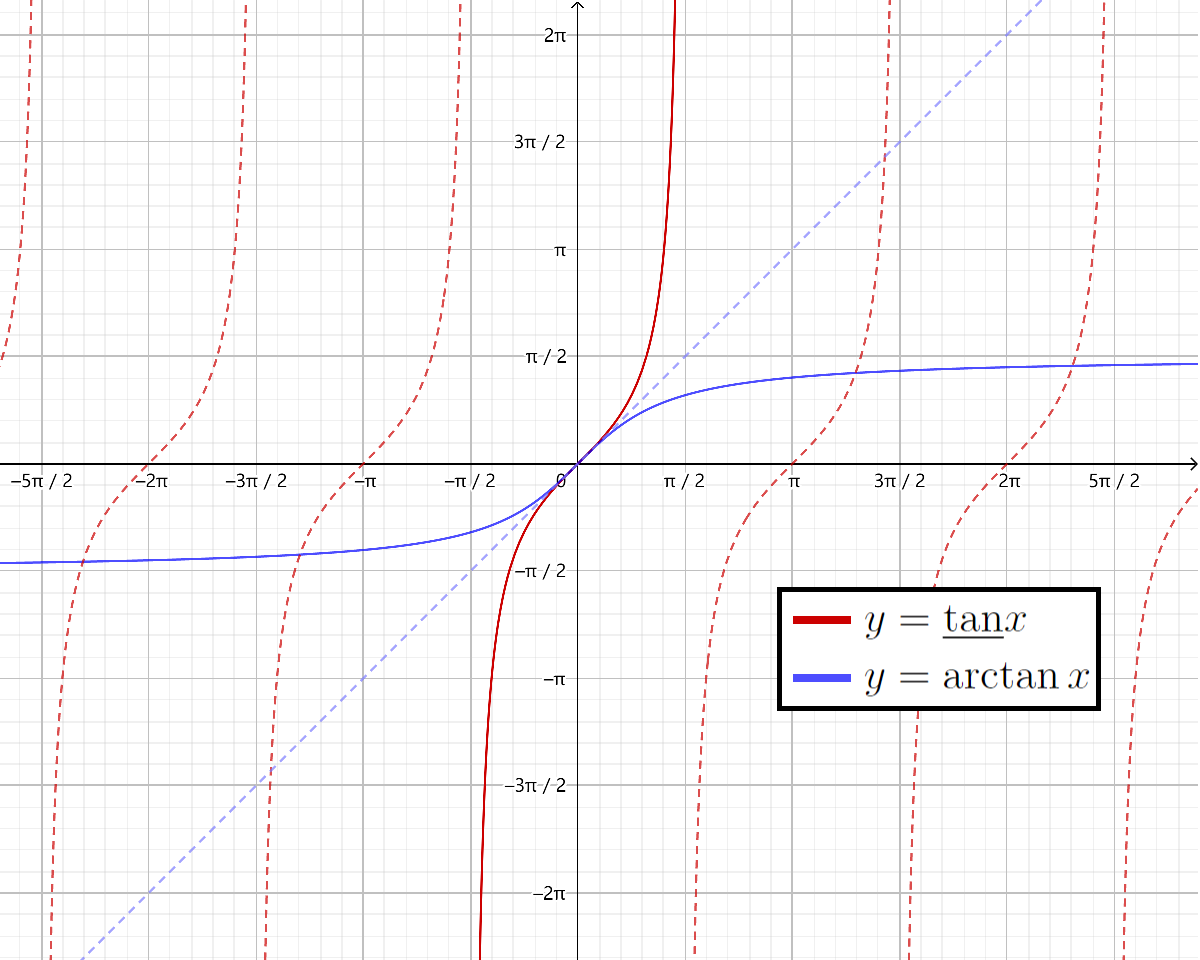
\includegraphics[width=0.8\textwidth]{反正切函数1.png}
    \caption*{\texttt{反正切函数}$x\mapsto \arctan(x)$}
\end{figure}

从图像中可以看出,反正切函数也是严格单调递增的函数。它的定义域是$\mathbb{R}$、值域是$(-\frac{\pi}{2}, \,\, \frac{\pi}{2})$。
$\underline{\tan}$是奇函数,因此,反正切函数也是奇函数。
$x > 0$时,反正切函数总大于$0$,增长越来越慢;$x < 0$时,反正切函数总小于$0$,增长越来越快。

举例来说,$\arctan{0} = 0$,$\arctan{1} = \frac{\pi}{4}$,
$\arctan{(-1)} = -\frac{\pi}{4}$,$\arctan{\sqrt{3}} = \frac{\pi}{3}$,$\arctan{\frac{\sqrt{3}}{3}} = \frac{\pi}{6}$,等等。

反正切函数的定义域是正切函数的值域。因此,$\tan{(\arctan{x})} = x$对任何实数总成立。
但反正切函数的值域只是正切函数的定义域的真子集,因此,$\arctan{(\tan{x})} = x$只对$(-\frac{\pi}{2}, \,\, \frac{\pi}{2})$中的数成立。

最后来看余切函数的反函数。余切函数的最小正周期是$\pi$,在$(0, \,\, \pi)$上严格单调递减。
我们把余切函数在这个区间上的部分记作$\underline{\cot}$:
\begin{align}
    \underline{\cot} : (0, \,\, \pi) &\rightarrow \mathbb{R} \notag \\
                                   x &\mapsto \cot{x} \notag
\end{align}
画出它的图像,按照直线$l: y = x$作对称,就得到它的反函数,称为\textbf{反余切函数},记作$\arccot$:
$$ \arccot : \mathbb{R} \rightarrow (0, \,\, \pi) . $$

\begin{figure}[h] %this figure will be at the right
    \vspace{4pt}
    \centering
    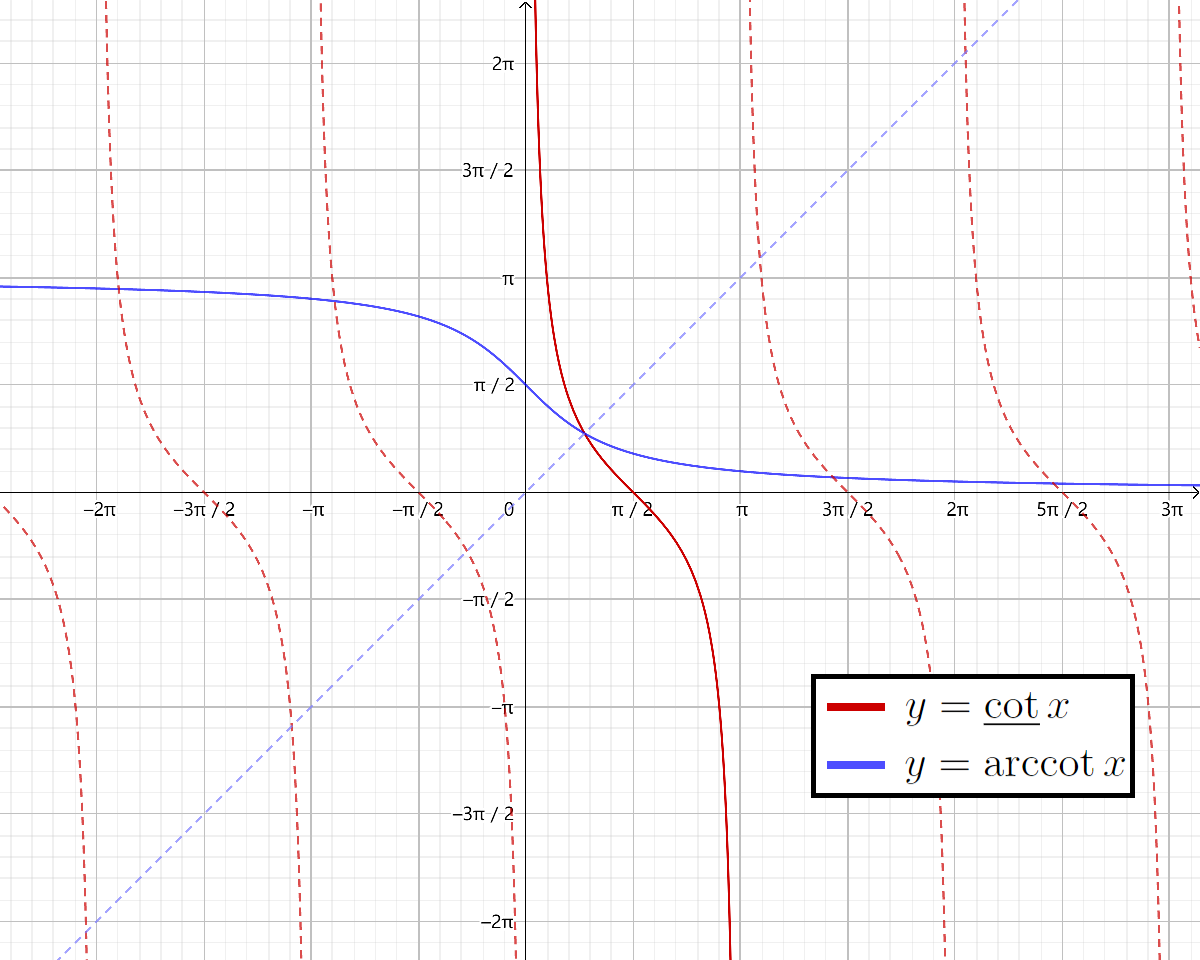
\includegraphics[width=0.8\textwidth]{反余切函数1.png}
    \caption*{\texttt{反余切函数}$x\mapsto \arccot(x)$}
\end{figure}

从图像中可以看出,反余切函数也是严格单调递减的函数。它的定义域是$\mathbb{R}$、值域是$(0, \,\, \pi)$。
$x < 0$时,反余切函数总大于$\frac{\pi}{2}$,减少得越来越快;$x > 0$时,反余切函数总小于$\frac{\pi}{2}$,减少得越来越慢。

举例来说,$\arccot{0} = \frac{\pi}{2}$,$\arccot{1} = \frac{\pi}{4}$,
$\arccot{(-1)} = \frac{3\pi}{4}$,$\arccot{\sqrt{3}} = \frac{\pi}{6}$,$\arccot{\frac{\sqrt{3}}{3}} = \frac{\pi}{3}$,等等。

反余切函数的定义域是余切函数的值域。因此,$\cot{(\arccot{x})} = x$对任何实数总成立。
但反余切函数的值域只是余切函数的定义域的真子集,因此,$\arccot{(\cot{x})} = x$只对$(0, \,\, \pi)$中的数成立。

\begin{sk}
    \mbox{} \\
    \indent 1. 能否找到别的区间来定义反正弦函数?能否找到比$[-\frac{\pi}{2}, \,\, \frac{\pi}{2}]$更长的区间?这样定义的反正弦函数有什么不同?\\
    \indent 2. 能否找到别的区间来定义反余弦函数?能否找到比$[0, \,\, \pi]$更长的区间?这样定义的反余弦函数有什么不同?\\
    \indent 3. 能否找到别的区间来定义反正切函数?能否找到比$(-\frac{\pi}{2}, \,\, \frac{\pi}{2})$更长的区间?这样定义的反正切函数有什么不同?\\
    \indent 4. 能否找到别的区间来定义反余切函数?能否找到比$(0, \,\, \pi)$更长的区间?这样定义的反余切函数有什么不同?\\
    \indent 5. 能否定义正割函数和余割函数的反函数?它们有什么特性?
\end{sk}
\begin{xt}
    \mbox{} \\
    \indent 1. 为什么说“$\underline{\sin}$是奇函数,因此,反正弦函数也是奇函数”?这个说法对一般的函数也成立吗?\\
    \indent 2. 考虑函数$x\mapsto \arcsin{(\sin{x})} - x$,它对哪些实数有定义?画出它在$[-\pi, \,\, \pi]$上的图像。它是周期函数吗?能否将它表示为简单函数和周期函数的和?\\
    \indent 3. 考虑函数$x\mapsto \arctan{(\tan{x})} - x$,它对哪些实数有定义?画出它在$[-\pi, \,\, \pi]$上的图像。它是周期函数吗?能否将它表示为简单函数和周期函数的和?\\
    \indent 4. 考虑函数$x\mapsto \cos(2x - 1)$,它在什么区间上可以定义反函数?如何用反三角函数表示这个反函数?
\end{xt}

\chapter{数列的极限}

我们来考察以下数列:
$$ 0,\,\, \frac{1}{2}, \,\,\frac{2}{3},\,\, \frac{3}{4}, \,\,\frac{4}{5}, \,\,\frac{5}{6}, \cdots $$
它的通项公式是$a_n = \frac{n-1}{n}$。
把数列的前几项在数轴上标出来,我们发现:
随着$n$不断增大,$a_n$不断变大,不断向着$1$靠拢。

数列$\{a_n\}$各项随着$n$增大,不断接近$1$。
虽然数列任一项都不等于$1$,但我们不难产生这样的想法:随着$n$增大,$a_n$的值任意接近于$1$。

怎样严谨地表达这个想法呢?我们使用“有求必应”和“一路全真”的结构,把上面的想法用更具体的方式来描述。
直观来看,我们考察以$1$为中心的区间$[1-r,1+r]$,
无论这个区间多么小,到了一定的$n$以后,所有的$a_n$都会落在这个区间里。

用二元命题$Q(r, n)$表示“$a_n$落在区间$[1-r,1+r]$里”。
用类似“有求必应”的结构,以上的想法可以写成:
$$\forall r > 0, \,\,\, \exists n,  \,\,\, \mbox{使得} \forall \,\, m \geqslant n, \,\,\, Q(r, n)\mbox{成立。}$$
这个结构比“有求必允”结构要求更高。它不仅要求“必允”,而且一旦“允”了,就要求之后“一路全真”。
用表格来表示这个结论:

\begin{figure}[h] %this figure will be at the right
    % \vspace{4pt}
    \centering
    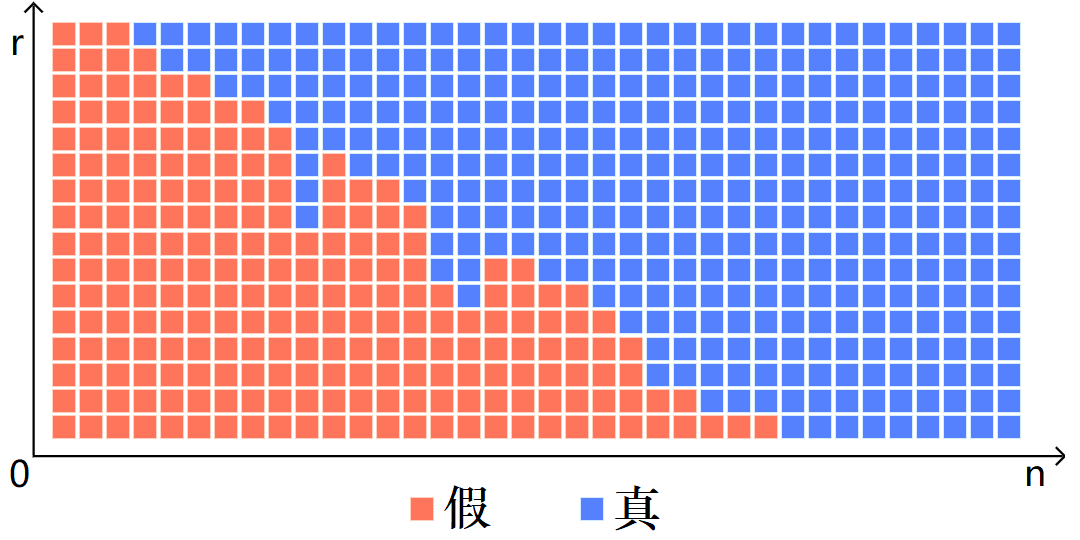
\includegraphics[width=0.64\textwidth]{数列极限2.png}
\end{figure}

每格颜色对应$Q(r, n)$的真假。每一行对应一个正数$r$,每一列对应数列的一个下标$n$。我们的想法是:
不论$r>0$是多少,它对应的行中,$Q(r, n)$必然从某一列起全为真。

我们把$1$称为数列$\{a_n\}$的\textbf{极限}。对一般数列来说,我们定义:
\begin{df}\textbf{数列的极限} \\
设有无穷数列$\{a_n\}$,其元素属于数集$T$。如果有某个数$x$,使得
$$ \forall r\in T, \,\, r > 0, \,\,\, \exists n,  \,\,\, \mbox{使得} \,\,\, \forall \,\, m \geqslant n, \,\,\, - r \leqslant a_m - x \leqslant r. $$
就说$\{a_n\}$有极限$x$,或$x$是$\{a_n\}$的极限,或$\{a_n\}$趋于$x$,或$\{a_n\}$收敛到$x$,记作
$$\{a_n\} \to x.$$
数列有极限也称为数列\textbf{收敛},数列没有极限也称数列\textbf{不收敛}。
\end{df}

\begin{figure}[h] %this figure will be at the right
    \vspace{-14pt}
    \centering
    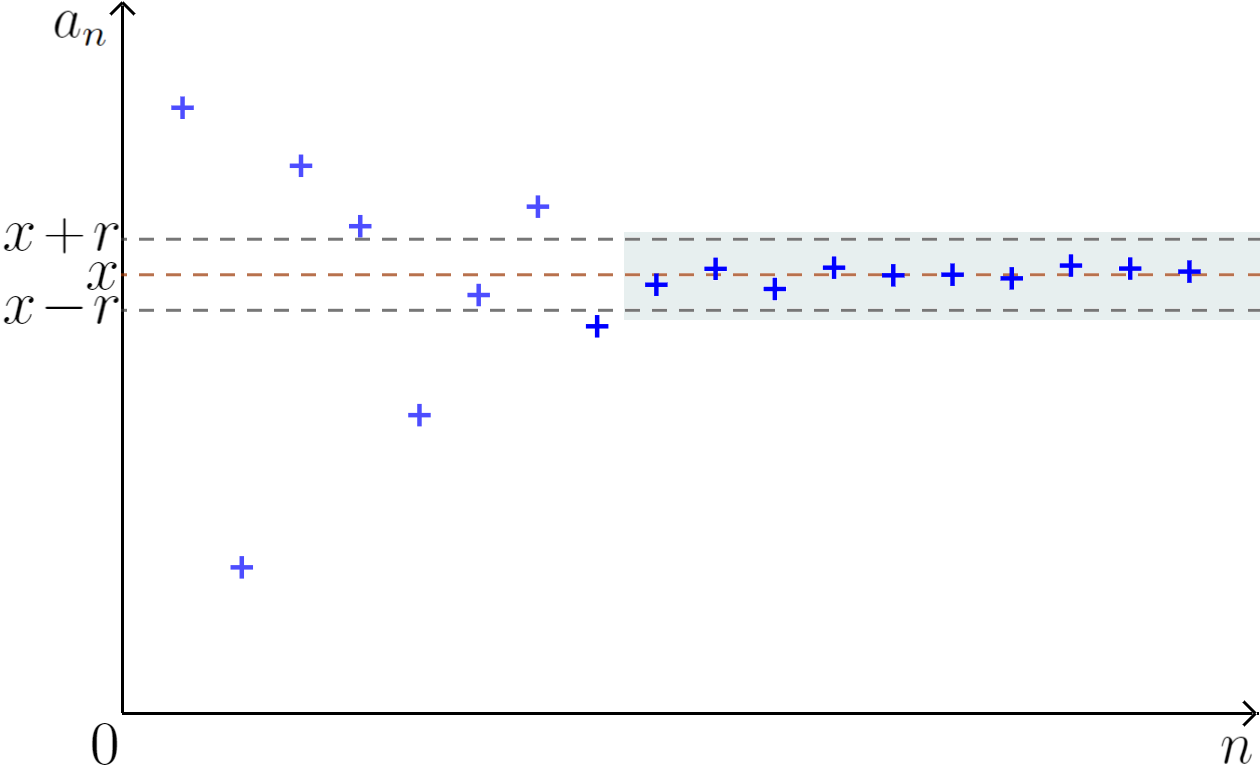
\includegraphics[width=0.54\textwidth]{数列极限1.png}
    \caption*{\texttt{从某一项开始,数列的值总落在区间}$[x-r,x+r]$\texttt{中}}
\end{figure}

\begin{et}
数列$\{a_n\}$的通项是$a_n = \frac{1}{n^2}$,它是否有极限?如果有极限,极限是多少?    
\end{et}
\begin{so}
    $\{a_n\}$每项都是正数。
    $$a_{n} \div a_{n+1} = \frac{1}{n^2} \div \frac{1}{(n+1)^2} = \frac{(n+1)^2}{n^2} = 1 + \frac{2n+1}{n^2} > 1,$$
    所以$\{a_n\}$是单调递减数列。从数轴上看,$\{a_n\}$不断趋近于$0$。猜测它有极限$0$。\\
    设$r>0$,考察区间$[-r,r]$。设$n_r$是大于等于$\frac{1}{\sqrt{r}}$的最小正整数,
    那么,只要$n \geqslant n_r$,就有$n^2 \geqslant n_r^2 \geqslant \frac{1}{r}$,
    于是$0 \leqslant \frac{1}{n^2} \leqslant r$。因此,$\forall r > 0$,$\exists n_r$,
    使得$\forall m \geqslant n_r$,$ -r  \leqslant a_m - 0 \leqslant r$。这说明$\{a_n\}$有极限$0$。    
\end{so}

\section{极限的基本性质}
不难看出,极限是构造出来的。因此,从定义出发,我们可以说某个数是某数列的极限。
反过来,一个数列有极限,它的极限是否只能有一个呢?答案是肯定的。我们可以用反证法来证明。

反设某数列$\{a_n\}$有两个极限$x_1, x_2$。不妨设$x_1 < x_2$。直觉上,$n$足够大的时候,$a_n$在数轴上离$x_1, x_2$都很近,
到两点的距离比$x_2 - x_1$的一半都小,加起来就小于$x_2 - x_1$,于是就产生矛盾了。

具体来说,记$\delta = \frac{x_2 - x_1}{2}$为两点距离的一半。选一个小于$\delta$的正数$r$。
按照极限的定义,有正整数$n_1, n_2$使得:
\begin{align}
    \forall m \geqslant n_1 , \,\,\,& -r \leqslant a_m - x_1 \leqslant r , \notag \\
    \forall m \geqslant n_2 , \,\,\,& -r \leqslant a_m - x_2 \leqslant r . \notag 
\end{align}
于是,选一个比$n_1,n_2$都大的$m$,比如$m=n_1+n_2$,这时$a_m - x_1 \leqslant r$,$x_2 - a_m \leqslant r$。
加起来就得到:
$$x_2 - x_1 \leqslant 2r < 2\delta = x_2 - x_1.$$
矛盾!因此,\textbf{数列如果有极限,只能有一个极限。}

数列的极限,如果存在,是唯一的。我们可以把数列$\{a_n\}$的极限记为$a_\infty$。如果要讨论数列和它的极限之间的关系,
我们可以把这个关系看作一种映射,称为\textbf{极限映射}或\textbf{取极限的操作}。
比如,实数构成的数列与其极限的关系,可以写成:
\begin{align}
    \lian{} : \,\,\, \mathbb{R}^\mathbb{N} &\longrightarrow \mathbb{R} \notag \\
    \{a_n\} &\longmapsto a_\infty \notag
\end{align}

设数列$\{a_n\}$有极限$a_\infty$。我们把它每一项减去$a_\infty$,
得到的数列$\{a_n - a_\infty\}$趋于$0$。所以,任何有极限的数列,都可以看做一个趋于$0$的数列加上它的极限。
我们把趋于$0$的数列称为\textbf{无穷小}。任何有极限的数列,都是它的极限加上无穷小。

极限描述了数列的项在“远处”的特征。我们把数列下标超过一定限度后的特征称为数列的\textbf{大体行为}。
有极限的数列,我们可以用极限来刻画数列的大体行为(落在极限“附近”)。
没有极限的数列,大体行为有什么特征呢?

我们来看另一个数列:
$$ 1,\,\,2,\,\,3,\,\,4,\,\,5,\cdots $$
它是正整数数列,通项为$a_n = n$。不难看出,它没有极限。因为对任何实数$x$来说,
令$n_x$为大于$x$的最小正整数,那么从$n_x+1$开始的项都比$x$大至少$1$,
无法落到$x$附近的小区间里面。可以说,随着$n$增大,$a_n$会比任何数都大。

如何严谨描述这个想法呢?我们仍然可以用“有求必应”的结构,把以上想法写成:
$$ \forall x, \,\,\, \exists n, \,\,\,\mbox{使得} \,\,\,\forall \,\, m \geqslant n,,\,\,\, a_m \geqslant x.$$
直观来看,随着$n$增大,从某一项开始,$a_n$会落到数轴任何给定点$x$的右边。
我们把这个性质称为数列\textbf{趋于正无穷大}。同理,可以定义数列\textbf{趋于负无穷大}:
$$\forall x, \,\,\, \exists n, \,\,\,\mbox{使得}\,\,\,\forall \,\, m \geqslant n,,\,\,\, a_m \leqslant x.$$
直观来看,随着$n$增大,从某一项开始,$a_n$会落到数轴任何给定点$x$的左边。

\begin{wrapfigure}[9]{r}{0.33\textwidth} %this figure will be at the right
    \vspace{-48pt}
    \flushright
    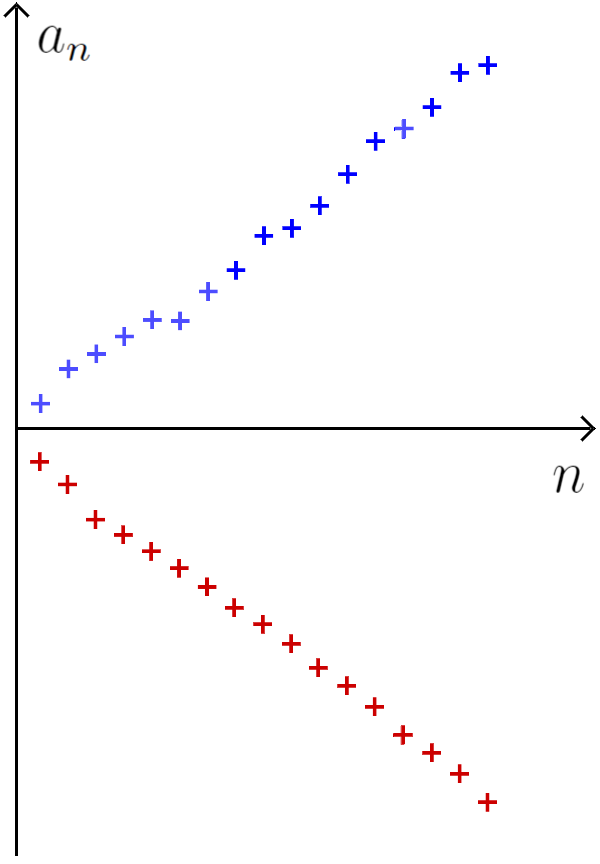
\includegraphics[width=0.32\textwidth]{数列无穷大1.png}
    \caption*{\texttt{趋于无穷大的数列}}
\end{wrapfigure}

我们也把有这两个性质的数列简称为\textbf{正无穷大}和\textbf{负无穷大},合称\textbf{无穷大}。

\begin{et}
    设数列$\{\frac{1}{n}\}$的部分和数列为$\{a_n\}$,证明:$\{a_n\}$趋于正无穷大。
\end{et}
\begin{proof}
    按照定义,$ a_n = 1 + \frac{1}{2} + \cdots + \frac{1}{n}$。\\
    $a_{n+1} - a_n = \frac{1}{n+1} > 0$,所以$\{a_n\}$单调递增。\\
    对任意实数$x$,我们需要找到相应的$n$,使得$\forall m \geqslant n$,$a_m \geqslant x$。
    由于$\{a_n\}$单调递增,只要某一项$a_n \geqslant x$,它之后的项都大于等于$x$。
    因此,只需要找到$n$使得$a_n \geqslant x$即可。\\
    如果$x \leqslant 1$,那么$n=1$即满足要求。\\
    如果$x > 1$,设$M$是大于$x$的最小整数,考虑$n = 2^{2M}$。下面证明$a_{2^{2M}}>x$。\\
    $$ a_{2^{2M}} = a_{2^0} + \sum_{i=1}^{2M}a_{2^i} - a_{2^{i-1}}.$$
    \begin{align}
        \forall \,\, i\in[1\ldots 2M],\,\,\, a_{2^i} - a_{2^{i-1}} &= \frac{1}{2^{i-1}+1} + \frac{1}{2^{i-1}+2} + \cdots + \frac{1}{2^{i}} \notag \\
        &\geqslant \frac{1}{2^{i}} + \frac{1}{2^{i}} + \cdots + \frac{1}{2^{i}} \notag \\
        &= \frac{2^{i-1}}{2^{i}} = \frac{1}{2}. \notag
    \end{align}
    $$ \mbox{所以}\quad  a_{2^{2M}} \geqslant a_1 + \frac{1}{2} \cdot (2M - 1) = M + \frac{1}{2} > x. $$
    这就证明$\{a_n\}$趋于正无穷大。
\end{proof}

极限作为反映数列大体行为的特征,也在一定程度上保留数列之间的关系。
最简单来说,如果数列$\{a_n\}$小于$\{b_n\}$,那么,如果俩数列都有极限$a_\infty$、$b_\infty$,
可以想象,$a_\infty$不应该比$b_\infty$大。反之亦然。

我们有这样的结论:
\begin{tm}
    设数列$\{a_n\}$、$\{b_n\}$分别有极限$a_\infty$、$b_\infty$。如果$\{a_n\}$小于(等于)$\{b_n\}$,那么$a_\infty\leqslant b_\infty$。
\end{tm}

我们把这个结论称为“极限传递不等关系”。要注意的是,极限无法传递严格的不等关系。即便数列$\{a_n\}$严格小于$\{b_n\}$,它们的极限也可能相等。

举例来说,考虑数列$\left\{\frac{1}{n}\right\}$和$\left\{-\frac{1}{n}\right\}$。前者每一项都是正的,后者每一项都是负的,因此前者每一项严格大于后者对应的项。
然而俩数列都趋于同一个极限:$0$。

我们看到两个数列中,一个数列每项都比另一个数列对应的项要大,但两者收敛到同一个极限。这种情况下,如果有第三格数列每项都在两者之间,那么由于“上下”都趋于同一个数,
第三个数列夹在其中,也只能趋于这个数了。这个结论称为\textbf{同归定理}。
\begin{tm}{\textbf{同归定理}}\label{tm:a-0-48}
    如果数列$\{a_n\}$小于(等于)$\{b_n\}$,$\{b_n\}$小于(等于)$\{c_n\}$,而$\{a_n\}$、$\{c_n\}$有同样的极限$x$,那么$\{b_n\}$也收敛到$x$。
\end{tm}
\begin{proof}
    按照定义,对任意正数$r>0$,存在正整数$N_a$,使得只要$n>N_a$,就有$|a_n - x| < r$。
    同理,存在正整数$N_c$,使得只要$n>N_c$,就有$|c_n - y| < r$。这说明,$n$大于$N_a,N_c$中较大者的时候,
    总有
    $$ x - r < a_n \leqslant b_n \leqslant c_n < x + r. $$
    因此$\{b_n\}$也收敛到$x$。
\end{proof}

\begin{sk}
    \mbox{} \\
    \indent 1. 张三在判定数列$\{a_n\}$的极限时写到:数$x$满足:
    $$ \forall r > 0, \,\,\, \exists n,  \,\,\, \mbox{使得} \forall \,\, m > n \,\,\, \mbox{都有} x - r < a_m < x + r. $$
    \indent 因此$\{a_n\}$有极限$x$。他的说法对吗?\\
    \indent 2. 李四在判定数列$\{a_n\}$的极限时写到:数$x$满足:
    $$ \forall r > 0, \,\,\, \exists n,  \,\,\, \mbox{使得} \forall \,\, m > n \,\,\, \mbox{都有} x - 2r \leqslant a_m \leqslant x + 2r. $$
    \indent 因此$\{a_n\}$有极限$x$。他的说法对吗?\\
    \indent 3. 一般数列除了有极限和趋于正/负无穷大,还可能有什么大体行为?\\
    \indent 4. 单调数列除了有极限和趋于正/负无穷大,还可能有什么大体行为?
\end{sk}

\begin{xt}
    \mbox{} \\
    \indent 1. 以下数列是否有极限?如果有极限,是多少?\\
    \indent\indent 1.1. $\{2^{1-n}\}$ \\
    \indent\indent 1.2. $\{(-1)^{n-1}\frac{n+1}{3n+1}\}$ \\
    \indent\indent 1.3. $\{1 - \frac{1}{n^3+1}\}$ \\
    \indent 2. 以下数列是否趋于无穷大?\\
    \indent\indent 2.1. $\{2^{n}\}$ \\
    \indent\indent 2.2. $\{n^2\}$ \\
    \indent\indent 2.3. $\{\frac{2^n}{n^2}\}$\\
    \indent 3. 用反证法证明:如果数列$\{a_n\}$有极限$a_\infty$,且数列的每一项都小于等于数$c$,则$a_\infty \leqslant c$。\\
    \indent 4. 用反证法证明:如果数列$\{a_n\}$有极限$a_\infty$,且数列的每一项都小于数$c$,则$a_\infty \leqslant c$。\\
    \indent 5. 如果数列$\{a_n\}$趋于$x$(趋于正/负无穷大),证明:$\{a_n\}$的任何子列趋于$x$(趋于正/负无穷大)。\\
    \indent 6. 证明:如果数列$\{a_n\}$大于等于趋于正无穷大的数列,那么$\{a_n\}$也趋于无穷大。\\
    \indent 7. 求数列$\{\sqrt{n^2 + n + 1} - n\}$的极限。\\
    \indent 7.1. 证明:$\forall n,\,\,\, \sqrt{n^2 + n + 1} - n > \frac{1}{2}$。\\
    \indent 7.2. 证明:$\forall n,\,\,\, \sqrt{n^2 + n + 1} - n < \frac{n + 1}{2n + 1}$。\\
    \indent 7.3. 使用同归定理证明$\{\sqrt{n^2 + n + 1} - n\}$趋于$\frac{1}{2}$。
\end{xt}

\section{极限的运算}
我们已经学习了数列的运算。数列之间可以做加法、减法、乘法。
如果数列$\{a_n\}$、$\{b_n\}$有极限,它们的和、差、乘积是否有极限?
答案是肯定的,并且符合我们的直觉:
\begin{tm}
    若数列$\{a_n\}$趋于$a$,$\{b_n\}$趋于$b$,则
    \begin{align}
        \lim_{n\to\infty} a_n \pm b_n &= a \pm b, \notag \\
        \lim_{n\to\infty} a_n \cdot b_n &= a \cdot b. \notag 
    \end{align}
\end{tm}
特别地,令$\{b_n\}$是常数列,就得到数乘对极限的影响:若数列$\{a_n\}$趋于$a$,则
$$ \forall \,\, t \in \mathbb{R}, \,\,\,  \lim_{n\to\infty} t \cdot a_n = ta. $$
\begin{proof}
    \mbox{} \\
    首先证明极限的加法:设数列$\{a_n\}$趋于$a$,$\{b_n\}$趋于$b$。按照定义,$\forall r > 0$,
    由于$\frac{r}{2}>0$,总有正整数$n_a, n_b$,使得
    \begin{align}
        \forall \,\, m \geqslant n_a, \,\,\, & - \frac{r}{2} \leqslant a_m - a \leqslant \frac{r}{2}, \notag \\
        \forall \,\, m \geqslant n_b, \,\,\, & - \frac{r}{2} \leqslant b_m - b \leqslant \frac{r}{2}, \notag 
    \end{align}
    因此,
    \begin{align}
        \forall \,\, m \geqslant n_a + n_b, \,\,\, & -r = - \frac{r}{2} - \frac{r}{2} \leqslant a_m + b_m - a - b \leqslant \frac{r}{2} + \frac{r}{2} = r \notag 
    \end{align}
    于是数列$\{a_n\} + \{b_n\}$趋于$a + b$。\\
    接下来证明极限的数乘:设$t$为实数,数列$\{a_n\}$趋于$a$,则数列$\{t\cdot a_n\}$趋于$ta$。
    这样,数列$\{a_n\} - \{b_n\}$可以看作$\{a_n\} + \{-1\cdot b_n\}$,因而趋于$a - b$。\\
    分两种情况讨论。如果$t=0$,那么$\{t\cdot a_n\} = \{0\}$,显然趋于$0$,也就是$ta$。
    如果$t \neq 0$,按照定义,对$\forall r > 0$,由于$\frac{r}{t} > 0$,总有正整数$n$使得
    $$ \forall \,\, m \geqslant n, \,\,\, a - \frac{r}{t} \leqslant a_m \leqslant a + \frac{r}{t}. $$
    因此
    $$ \forall \,\, m \geqslant n, \,\,\, ta - r \leqslant t\cdot a_m \leqslant ta + r. $$
    这就说明数列$\{t\cdot a_n\}$趋于$ta$。\\
    最后证明极限的乘法:设数列$\{a_n\}$趋于$a$,$\{b_n\}$趋于$b$。按照定义,$\forall r > 0$,
    取$r$与$1$的较小者,记为$r_1$。由于$r_1>0$,总有正整数$n_a, n_b$,使得
    \begin{align}
        \forall \,\, m \geqslant n_a, \,\,\, & - r_1 \leqslant a_m - a \leqslant r_1, \notag \\
        \forall \,\, m \geqslant n_b, \,\,\, & - r_1 \leqslant b_m - b \leqslant r_1, \notag 
    \end{align}
    因此
    \begin{align}
        \forall \,\, m \geqslant n_a + n_b, \,\,\, & (a_m - a)(b_m - b) \leqslant r_1^2  \notag \\
        & -(a_m - a)(b_m - b) \leqslant r_1^2  \notag \\
        \mbox{即 }\quad & - r_1^2 \leqslant (a_m - a)(b_m - b) \leqslant r_1^2. \notag 
    \end{align}
    如果$r\geqslant 1$,那么$r_1=1$,因此$r_1^2 = 1 \leqslant r$;如果$0 < r <1$,那么$r_1 = r$,
    $r_1^2 = r^2 < r$。也就是说,任何情况下,总有$0 \leqslant r_1^2 \leqslant r$。于是:
    $$ -r \leqslant - r_1^2 \leqslant (a_m - a)(b_m - b) \leqslant r_1^2 \leqslant r $$
    这说明数列$\{(a_n - a)(b_n - b)\}$趋于$0$。而$\{b\cdot a_n\}$和$\{a \cdot b_n\}$都趋于$ab$,
    常数列$\{ab\}$也趋于$ab$,所以根据前面证明的极限加减法,数列
    $$\{a_nb_n\} = \{(a_n - a)(b_n - b)\} + \{b\cdot a_n\} + \{a \cdot b_n\} - \{ab\}$$
    趋于$0 + ab + ab - ab = ab$。
\end{proof}

四则运算中,加法、减法、乘法都可以对数列的极限做运算。那么除法是否可以呢?
具体来说,若数列$\{a_n\}$趋于$a$,$\{b_n\}$趋于$b$,是否有$\{\frac{a_n}{b_n}\}$趋于$\frac{a}{b}$?

显然,$b=0$的时候,$\frac{a}{b}$无定义,所以先考虑$b$不等于$0$的情况。这时答案大致是肯定的。
$\{\frac{a_n}{b_n}\}$趋于$\frac{a}{b}$。
当然,我们要先“剪掉”$\{b_n\}$最开始一些离$b$比较远的项,确保剩下的项都不等于$0$,这样才好定义$\frac{a_n}{b_n}$。
然后可以用类似证明极限乘法的方法,证明$\{\frac{1}{b_n}\}$趋于$\frac{1}{b}$,
这样,$\{\frac{a_n}{b_n}\}$可以看作$\{a_n \cdot \frac{1}{b_n}\}$,因而趋于$\frac{a}{b}$。

如果$b=0$,即数列$\{b_n\}$为无穷小,那么我们需要考虑的问题就更多了。首先考虑$a\neq 0$的情况。
像前面一样,$\{b_n\}$中等于$0$的项会使得$\frac{a_n}{b_n}$无法定义。
所以我们要确保$\{b_n\}$中没有$0$。其次,我们选择一个很小的正数,比如$r=\frac{a}{101}$。
根据定义,存在正整数$N$,使得对所有$n>N$,$|b_n| \leqslant r$、$|a_n - a| \leqslant r$。
于是,$N$以后的项$\frac{a_n}{b_n}$的绝对值总大于等于$\frac{a - r}{r} = 100$。
然而,这时$a_n$和$b_n$的情况还不一样。$a_n$和$a$相近,因此符号不变。$b_n$则可正可负。
因此,$\frac{a_n}{b_n}$的符号是随着$b_n$改变的。也就是说,$N$项以后,$\frac{a_n}{b_n}$也许会大于等于$100$,
也许会小于等于$-100$。如果这样,数列显然没有极限。

于是,我们对$\{b_n\}$再加一个限制:从某一项开始,$\{b_n\}$的项正负号不变。

这时,根据上面的讨论,可以证明,从某一项开始,$\frac{a_n}{b_n}$的正负号保持不变。
注意到,上面的讨论中把$100$改成任意正数$M$,结论不变。所以,我们实际上已经证明,$\frac{a_n}{b_n}$的绝对值趋于正无穷大。
因此,要么从某一项开始,$\frac{a_n}{b_n}$总大于$0$,因此趋于正无穷大;
要么从某一项开始,$\frac{a_n}{b_n}$总小于$0$,因此趋于负无穷大。

最后考虑$a$也是$0$的情况。这种情况下,不论从哪一项开始,$a_n$、$b_n$都可正可负。
这时,$\{\frac{a_n}{b_n}\}$的大体行为取决于$a_n$、$b_n$之间的关系,不再是可以统一处理的问题。
我们把这种情况下的$\{\frac{a_n}{b_n}\}$称为关于数列$\{a_n\}$和$\{b_n\}$的\textbf{不定式}。
关于数列$\{a_n\}$和$\{b_n\}$的不定式是否有极限,极限是什么,要根据具体情况来讨论。

综上所述,有极限的数列$\{a_n\}$、$\{b_n\}$的商数列$\{\frac{a_n}{b_n}\}$的大体行为,可以概括为:
\begin{center}
    \fbox{
        \shortstack[l]{
            设数列$\{a_n\}$的极限为$a$。\\
            1. 如果$\{b_n\}$的极限$b\neq 0$,那么$\{\frac{a_n}{b_n}\}$收敛到$\frac{a}{b}$。\\
            2. 如果$\{b_n\}$的极限$b = 0$,那么:\\
            \quad 1. 如果$a \neq 0$,那么:\\
            \quad \quad 1. 如果从某一项起,$b_n$总与$a$同号,那么$\{\frac{a_n}{b_n}\}$趋于正无穷大。\\
            \quad \quad 2. 如果从某一项起,$b_n$总与$a$异号,那么$\{\frac{a_n}{b_n}\}$趋于负无穷大。\\
            \quad \quad 3. 否则$\{\frac{a_n}{b_n}\}$没有极限。\\
            \quad 2. 如果$a = 0$,那么$\{\frac{a_n}{b_n}\}$为不定式。
        }
    }
\end{center}

\begin{sk}
    \mbox{} \\
    \indent 1. 如果数列$\{a_n\}$有极限$a$,$\{b_n\}$趋于无穷大,它们的和、差、积、商数列是否有极限?是否趋于无穷大?\\
    \indent 2. 如果数列$\{a_n\}$有极限$a$,$\{b_n\}$没有极限,也不趋于无穷大,它们的和、差、积、商数列是否有极限?\\
    \indent 3. 如果数列$\{a_n\}$、$\{b_n\}$都趋于无穷大,它们的和、差、积、商数列有什么特性?
\end{sk}

\section{极限和实数}
\begin{center}
    \fbox{
        \shortstack[l]{
            由于本节需要处理的证明细节过多,\\
            证明过程参见\textbf{附录:从数列到实数}的对应部分。
        }
    }
\end{center}

学习无限循环小数的时候,我们思考过这样的问题:$0.\dot{9}$是什么数?它有多大?

$0.\dot{9}$的问题,引发了这样的思考:什么是数?当我们按任意方式书写数字符号(包括小数点、循环节等)的时候,
我们是否总能知道我们写的东西是有意义的?

目前,我们学过的数有自然数、整数、有理数和实数。其中,整数是自然数的减法延伸得到的,有理数是整数的除法延伸得到的。
那么,实数和它们之间的关联是怎样的呢?

从开方运算得到无理数$\sqrt{2}$开始,我们承认了有理数不是所有的数。我们将有理数和无理数统称为实数。
另一方面,我们把直观的长度(及其相反数)抽象为实数。我们对“数”的认识一方面来自于数数,
一方面来自于客观现实中的测量:长度、面积、体积、温度等等。这两种“数”是否是统一的呢?
更重要的:实数是否是所有的数?怎样的数是实数?实数是怎样的数?其本质是什么?

这是一个深刻的问题。让我们首先回顾有理数和整数的关系。我们可以用整数定义有理数。给定有理数$r$,它总是某个整数$p$除以正整数$q$的商。
另一方面,给定整数$p$和正整数$q$,其商$\frac{p}{q}$总是有理数。也就是说,我们有这样一个映射:
\begin{align}
    L: \mathbb{Z} \times \mathbb{Z}^+ &\rightarrow \mathbb{Q} \notag \\
    (p, \,\, q) &\mapsto \frac{p}{q} \notag
\end{align}
映射$L$是满射,但不是单射。我们可以这样修改映射$L$:考虑所有有序数对$(p, \,\, q)$($q\neq 0$)构成的集合$\mathbb{Z} \times \mathbb{Z}^+$里的二元关系:
$$ (a,\,\, b) \leftrightarrows (c, \,\, d)\quad \mbox{当且仅当} \quad a\cdot d = b \cdot c.$$
可以证明,二元关系$\leftrightarrows$是等价关系:
\begin{enumerate}
    \item $\forall \,\, a\in \mathbb{Z}, \,\, b\in\mathbb{Z}^+, \,\,\, (a,\,\, b) \leftrightarrows (a, \,\, b)$。
    \item $\forall \,\, a,c\in \mathbb{Z}, \,\, b,d\in\mathbb{Z}^+$,如果$(a,\,\, b) \leftrightarrows (c, \,\, d)$,则$ (c, \,\, d)\leftrightarrows (a,\,\, b)$。
    \item $\forall \,\, a,c,e\in \mathbb{Z}, \,\, b,d,f\in\mathbb{Z}^+$,如果$(a,\,\, b) \leftrightarrows (c, \,\, d)$、$ (c, \,\, d)\leftrightarrows (e,\,\, f)$,则$(a,\,\, b) \leftrightarrows (e,\,\, f)$。
\end{enumerate}
因此,我们可以定义等价类$\overline{(p,\,\, q)}$。不难证明,每个有理数恰好对应一个这样的等价类。此外,我们还可以定义这些等价类上的四则运算:
\begin{itemize}
    \item $\overline{(a,\,\, b)} \pm \overline{(c, \,\, d)} = \overline{(ad \pm bc, \,\, bd)}.$
    \item $\overline{(a,\,\, b)} \times \overline{(c, \,\, d)} = \overline{(ac, \,\, bd)}.$
    \item $\overline{(a,\,\, b)} \div \overline{(c, \,\, d)} = \overline{(ad, \,\, bc)}.$
\end{itemize}
可以证明,这样定义的四则运算同样满足加法结合律、乘法结合律、加法交换律、乘法交换律,以及乘法对加法的分配律。

这说明,我们定义的等价类$\overline{(p,\,\, q)}$和有理数一模一样,只是记法不同。我们说这样定义的等价类,作为代数系统,与有理数\textbf{同构}。
或者说,我们用以上的方法定义了我们熟知的“有理数和四则运算”这个代数系统。

那么,对实数来说,我们能不能从有理数出发,定义“实数和四则运算”呢?下面,让我们用数列的极限来定义实数。

\subsection{自敛数列}

考虑数列$\{a_n\}$:
$$ a_1 = 1, \quad \forall \,\, n \in \mathbb{Z}^+, \,\,\, a_{n+1} = \frac{a_n}{2} + \frac{1}{a_n} $$
$\{a_n\}$的项是有理数四则运算的结果,所以总是有理数。用归纳法可以证明,$1 \leqslant a_n \leqslant 2$总成立。此外可以验证:
$$ a_{n+1} - \sqrt{2} = \frac{(a_n - \sqrt{2})^2}{2a_n},$$
因此,
$$ |a_{n+1} - \sqrt{2}| = \frac{|a_n - \sqrt{2}|}{2|a_n|} \cdot |a_n - \sqrt{2}| < \frac{2 - \sqrt{2}}{2} \cdot |a_n - \sqrt{2}| < 0.3\cdot |a_n - \sqrt{2}|. $$
这说明总有$|a_n - \sqrt{2}| < (0.3)^{n-1}$。于是$\{a_n\}$趋于$\sqrt{2}$。然而,$\sqrt{2}$并不是有理数。这说明有理数集合并不是致密的。
一列有理数互相靠近,自相收敛,但它们最终收敛的结果,是不属于有理数集合的“空隙”。

对有理数来说,“数列的极限”这个概念是不完备的:我们没法只通过有理数来讨论有理数列的极限。

另一方面,从直观上,我们可以把有理数列理解为对客观世界不断测量的结果。举例来说,我们用尺子测量一根树枝的长度,
把第$n$次测量的结果记为$a_n$,就得到一个数列。每次测量的结果是尺子最小刻度的倍数,即为有理数。
如果我们测量的手段越来越先进,尺子的最小刻度越来越小,而且测量的结果相互之间也越来越接近,
那么,我们就认为数列$\{a_n\}$在不断逼近树枝的真实长度。换句话说,每个实数,作为真实的长度,可以用相互之间不断靠近的测量结果来逼近。

我们来定义这样一种数列:
\begin{df}\textbf{自敛数列}
    如果随着$N$增大,数列$\{a_n\}$自第$N$项往后,各项之间的差任意小,就说数列$\{a_n\}$是\textbf{自敛}的(或者说$\{a_n\}$有\textbf{自敛性})。
    具体来说,给定数列$\{a_n\}$,其元素属于数集$T$,如果对$T$中任意正数$r$,都存在正整数$N$,
    使得对只要下标$k,m>N$,就有$|a_k - a_m| \leqslant r$,就说数列$\{a_n\}$是\textbf{自敛}的。
\end{df}

顾名思义,数列自敛,指数列的项逐渐相互靠近,自相收敛到一起。

\begin{et} 
    考察数列$\left\{\frac{1}{n}\right\}_{n\in\mathbb{Z}^+}$是否是自敛数列。\\
\end{et}
\begin{so}
    数列$\left\{\frac{1}{n}\right\}_{n\in\mathbb{Z}^+}$是单调递减数列,而且有下界$0$。任意给定$r>0$,设$r$写为既约分数$r = \frac{p}{q}$,
    我们可以取$N = q$。由于$p > 0$,总有$p \geqslant 1$,即$r \geqslant \frac{1}{N}$。因此,当$n\geqslant m>N$的时候,总有
    $$|a_n - a_m| = \frac{1}{m} - \frac{1}{n} < \frac{1}{m} < \frac{1}{N} \leqslant r.$$
    这说明$\left\{\frac{1}{n}\right\}_{n\in\mathbb{Z}^+}$是自敛数列。
\end{so}
\begin{et} 
    数列$\left\{a_n\right\}_{n\in\mathbb{Z}^+}$满足递推关系:
    $$a_1 = 2, \quad 2a_{n+1} = a_n + 1.$$
    \indent 考察$\left\{a_n\right\}_{n\in\mathbb{Z}^+}$是否是自敛数列。\\
\end{et}
\begin{so}
    注意到
    $$ a_{n+1} - 1 = \frac{1}{2}\cdot (a_n - 1). $$
    因此,$\{a_n - 1\}_{n\in\mathbb{Z}^+}$是等比数列。通项公式为:
    \begin{align}
        a_n - 1 &= \left(\frac12\right)^{n-1} (a_1 - 1) = \frac{1}{2^{n-1}} \notag \\
        a_n &= 1 + \frac{1}{2^{n-1}} \notag
    \end{align}
    数列$\left\{a_n\right\}_{n\in\mathbb{Z}^+}$单调递减,有下界$1$。任意给定$r>0$,设$r$写为既约分数$r = \frac{p}{q}$,我们可以取$N = q$。
    这时$r \geqslant \frac{1}{N}$。用归纳法可以证明,任意正整数$N$总小于$2^N$,因此,当$n\geqslant m>N$的时候,总有
    $$|a_n - a_m| = 1 + \frac{1}{2^{m-1}} - \left(1 + \frac{1}{2^{n-1}} \right) < \frac{1}{2^{m-1}} \leqslant \frac{1}{2^N} < \frac{1}{N} \leqslant r.$$
    这说明$\left\{a_n\right\}_{n\in\mathbb{Z}^+}$是自敛数列。
\end{so}

不难看出,\textbf{有极限的数列,总是自敛的},因为它的项会逐渐趋于它的极限,于是互相靠近,收敛到一起。
然而,从最开始的例子可以看出,自敛的有理数列,不一定收敛到有理数。我们用自敛的有理数列来定义实数:
\begin{po}\textbf{实数的根本性质}
    任何自敛的有理数列总有极限,我们把自敛有理数列的极限称为实数。
\end{po}

作为极限的实数,刻画了实数作为“测量结果”的本质。作为日常生活中的“长度”抽象得到的概念,实数应当具有这样的性质:任意的长度都是真实存在的,直尺上不可能有两点之间没有长度;
即便由于测量工具的局限,我们无法精确测量物体的长度,我们也相信,物体的长度可以通过测量逐渐逼近。
\textbf{实数代表了人类在自身尺度下对空间的朴素认知}。

\begin{sk}
    \mbox{}\\
    \indent 1. 自敛数列定义中的“$|a_k -a_m| \leqslant r$”能否改成“$|a_k -a_m| < r$”?两种定义是否有区别?\\
    \indent 2. 我们定义有理数列的极限时,是否用到了实数?\\
    \indent 3. 我们定义有理数列极限的四则运算时,是否用到了实数?
\end{sk}
\begin{xt}
    \mbox{}\\
    \indent 1.已知数列的通项公式或递推公式,证明数列是自敛数列:\\
    \indent 1.1. $\{\frac{1}{n^2}\}_{n\in\mathbb{Z}^+}$\\
    \indent 1.2. $a_1 = 2, \quad \forall \,\, n\in\mathbb{Z}^+, \,\,\, a_{n+1} = \frac{a_n}{2} + \frac{1}{2a_n}.$\\
    \indent 1.3. $\left\{\frac{\sin(n)}{n}\right\}_{n\in\mathbb{Z}^+}$ \\
    \indent 2. 证明:有极限的数列,总是自敛数列。\\
    \indent 3. 证明:自敛数列总是有界数列。
\end{xt}

以上我们用自敛有理数列的极限重新定义实数,这样定义的实数是否符合我们直观的认识呢?

首先,我们要说明有理数总是实数。这是因为常数列总是自敛数列。所以,给定任意有理数$r$,它作为常数列$\{r\}$的极限,就是实数。

其次,我们定义两个实数的相等关系。
\begin{df}
    设实数$a$是自敛有理数列$\{a_n\}$的极限,$b$是自敛有理数列$\{b_n\}$的极限。
    $a = b$当且仅当$\{a_n - b_n\}$趋于$0$。
\end{df}
可以证明,这样定义的相等关系是一种等价关系。由于有理数也是实数,实数的相等关系和有理数的相等关系是同一种关系。
这个等价关系把每个实数对应到一个等价类。这个等价类由所有趋于这个实数的自敛有理数列构成。

接下来定义两个实数的大小关系(也叫序关系)。
\begin{df}
    设实数$a,b$分别对应自敛有理数列的等价类$A,B$。
    如果对$A$中任何数列$\{a_n\}$、$B$中任何数列$\{b_n\}$,总有正整数$N$,使得$\{a_n - b_n\}$自第$N$项往后总大于$0$,就说$a>b$、$b<a$。
\end{df}
可以证明,这样定义的大小关系满足以下基本性质:
\begin{enumerate}
    \item $\forall a$,$a < a$不成立。
    \item $\forall a, b$,$a < b$,$a > b$,$a = b$恰有一个成立。
    \item $\forall a, b, c$,如果$a < b$、$b < c$,则$a < c$。
    \item $\forall a, b, c$,如果$a > b$、$b > c$,则$a > c$。
\end{enumerate}
此外还能证明,实数的相等、不等关系和有理数一致。

更关键的是定义实数的四则运算。为此,要证明以下结论:
\begin{tm}
    设实数$a,b$分别对应自敛有理数列的等价类$A,B$。
    \begin{itemize}
        \item 集合$\{\{a_n + b_n\} \, | \, \{a_n\}\in A,\,\, \{b_n\}\in B\}$是一个等价类,定义它对应的实数为$a + b$。
        \item 集合$\{\{a_n - b_n\} \, | \, \{a_n\}\in A,\,\, \{b_n\}\in B\}$是一个等价类,定义它对应的实数为$a - b$。
        \item 集合$\{\{a_n \times b_n\} \, | \, \{a_n\}\in A,\,\, \{b_n\}\in B\}$是一个等价类,定义它对应的实数为$a \times b$。
        \item 如果实数$b\neq 0$,那么集合$\{\{a_n \div b_n\} \, | \, \{a_n\}\in A,\,\, \{b_n\}\in B\}$是一个等价类,定义它对应的实数为$a \div b$。
    \end{itemize}  
\end{tm}
可以证明,这样定义的四则运算,满足加法结合律、乘法结合律、加法交换律、乘法交换律,以及乘法对加法的分配律,并且与实数的相等、不等关系兼容(具体证明参见附录一)。
这样就说明,把实数定义为自敛有理数列的极限,这样的定义满足我们以前对实数的直观认知。

最后,我们来讨论实数构成的数列,我们用同样的方法定义自敛实数列和实数列的极限。可以证明,
\begin{tm}
    自敛的实数列总有极限,极限为实数。
\end{tm}
而另一方面,有极限的数列总是自敛的。所以,\textbf{实数列如果有极限,总是实数}。
我们把这个性质称为\textbf{实数的完备性}或\textbf{致密性}。实数的完备性说明,实数不仅是自敛有理数列的极限,也是自敛实数列的极限。
我们说实数对于极限操作是\textbf{完备}的,不会像自敛有理数列那样出现极限不在数集里的问题。

实数的完备性说明,如果把极限看作运算,那么实数集对这种运算是封闭的,就如有理数集对四则运算是封闭的一样。
至此,我们具备了运用数列极限这个工具的坚实基础。数列极限可以成为我们研究实数的有力工具。

\begin{sk}
    \mbox{}\\
    1. 整数、有理数、实数中都有等价关系。对比这些等价关系,你发现了什么共同点?你认为这些共同点背后的原因是什么?\\
    2. $0.\dot{9}$是否存在?如何看待$0.\dot{9}$这样的数?
\end{sk}

\begin{xt}
    \mbox{} \\
    设有实数列$\{u_n\}_{n\in\mathbb{Z}^+}$。考虑如下定义的数列$\{v_n\}_{n\in\mathbb{Z}^+}$:
    $$ \forall \,\, n\in\mathbb{Z}^+, \,\,\, v_n = \frac{u_1 + u_2 + \cdots + u_n}{n}. $$
    \indent 1. 假设$\{u_n\}$趋于$0$。设$r>0$。\\
    \indent 1.1. 证明:存在正整数$n_0$,使得$n>n_0$时总有
    $$ \left| \frac{1}{n} \sum_{n_0+1}^n u_n \right| \leqslant \frac{n-n_0}{n}r.$$
    \indent 1.2. 证明:存在正整数$n_1$,使得$n>n_1$时总有$|v_n| \leqslant r$。\\
    \indent 2. 证明:只要$\{u_n\}$有极限$x$,那么$\{v_n\}$也趋于$x$。
\end{xt}

\subsection{数列的确界}
每个实数都对应多个收敛到它的数列。为了方便,我们希望用一类性质良好的数列来代表实数。

单调数列是一种简单的数列,单调递增数列中,每一项都大于等于前面的项;单调递减数列中,每一项都小于等于前面的项。能否用单调数列来代表实数呢?
我们来研究单调数列的大体行为。

以单调递增数列为例。我们已经见过有极限的单调递增数列和趋于正无穷大的单调递增数列。除此以外,还有别的可能性吗?

我们用“是否有上界”来分类讨论。如果单调递增数列$\{a_n\}$没有上界,则$\{a_n\}$趋于正无穷大。

\begin{figure}[h]
    \vspace{-4pt}
    \centering
    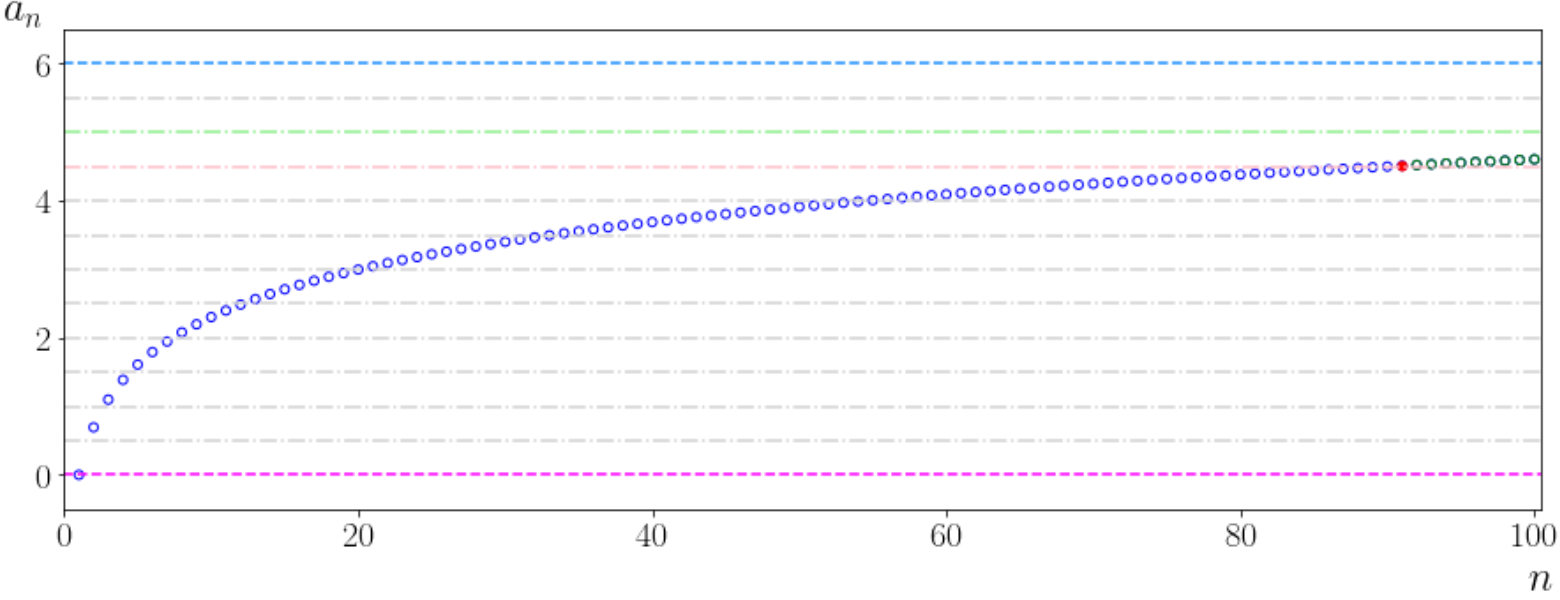
\includegraphics[width=0.84\textwidth]{上确界1.png}
\end{figure}

如果如果单调递增数列$\{a_n\}$有上界,即有某个有理数$M$,
使得$a_n < M$总成立。由于$a_n$随着$n$增大而增大,可以想象,增大会逐渐变缓乃至停滞。因此,$\{a_n\}$应该收敛于某个不大于$M$的数。

这个数显然在$a_1$和$M$之间。为了找出这个数,设定正整数$k$之后,我们把$M - a_1$这段距离均匀分成$k$份,记每份的大小为$r_k = \frac{M - a_1}{k}$。
从$a_1$出发,一步步“往$M$走”。每步的步长是$r_k$。一开始的时候,我们处于$a_1$的位置,$a_1$不是数列的上界,最终到达$M$,$M$是数列的上界。
因此,总有一步,从不是数列的上界走到数列的上界。

如果在第$i$步,$a_1 + i r_k$不是上界,而在第$i+1$步,$a_1 + (i+1) r_k$是上界。也就是说,有某一项$a_{N(k)}$大于等于$a_1 + i r_k$,
却小于$a_1 + (i+1) r_k$。由于数列单调递增,自$a_{N(k)}$开始的每一项都在$a_1 + i r_k$与$a_1 + (i+1) r_k$之间。这说明任两项的距离都小于$r_k$。

因此,对任何正数$r$,我们只要令$k$为大于$\frac{M - a_1}{r}$的正整数,就有
$r_k = \frac{M - a_1}{k} < r$。于是$\forall m,n\geqslant N(k)$,$|a_m - a_n|$总小于$r$。这说明$\{a_n\}$是自敛数列,因此有极限。

综上所述,单调递增数列要么趋于正无穷大,要么有极限。类似可以证明:单调递减数列要么趋于负无穷大,要么有极限。一个简单的判定法则是:
\begin{tm}\textbf{单调收敛定理}\label{tm:2-2-0}
    有上界(下界)的单调递增(递减)数列必然有极限。
\end{tm}
由于单调递增(递减)数列必然有下界(上界)$a_1$,单调收敛定理可以简化为:\textbf{有界单调数列收敛}。我们把有界单调数列的极限称为它的\textbf{确界}。
单调递增数列的极限叫做它的\textbf{上确界},单调递减数列的极限叫做它的\textbf{下确界}。

以单调递增数列来说,如果单调递增数列$\{a_n\}$有上界,设$a^{\text{上}}$为$\{a_n\}$上界的集合,那么上确界$a_\infty$就是其中最小的元素。证明如下:

首先证明$a_\infty \in a^{\text{上}}$。用反证法。反设$a_\infty$不是$\{a_n\}$的上界,则有某个$a_N$大于$a_\infty$,因此其后的项都大于$a_\infty$。即$n > N$时,
$a_n - a_\infty > a_N - a_\infty$。于是,对正数$a_N - a_\infty$来说,没有正整数$m$使得其后的项与$a_\infty$的差都小于等于$a_N - a_\infty$。
这与$\{a_n\}$趋于$a_\infty$矛盾!因此$a_\infty$是$\{a_n\}$的上界。

其次证明$\{a_n\}$的上界中没有比$a_\infty$更小的。仍然用反证法。反设$b \in a^{\text{上}}$是某个比$a_\infty$更小的上界:$b < a_\infty$。于是$a_n \leqslant b$总成立。也就是说,
$$\forall \,\, n, \,\,\, a_\infty - a_n = a_\infty - b + b - a_n \geqslant a_\infty - b.$$
这说明$\{a_n\}$所有的项和$a_\infty$的差都大于等于固定的正数$a_\infty - b$。于是,对正数$r = \frac{a_\infty - b}{2}$来说,没有正整数$m$使得其后的项与$a_\infty$的差都小于等于$r$。
这与$\{a_n\}$趋于$a_\infty$矛盾!因此$\{a_n\}$的上界中没有比$a_\infty$更小的。

综上所述,$a_\infty$是$a^{\text{上}}$中最小的元素,也称为数列的\textbf{最小上界},$a^{\text{上}}$可以表示为$[a_\infty, \,\,+\infty)$。

同样地,如果单调递减数列$\{a_n\}$有下界,那么下确界$a_\infty$就是$a_{\text{下}}$最大的元素,也称为数列的\textbf{最大下界},$a_{\text{下}}$可以表示为$(-\infty,\,\,a_\infty]$。 

确界的概念可以推广到一般的数的集合。给定非空的数集$S$,$S$的上(下)确界就是它的上(下)界集合中的最小(大)元素。
可以证明(见附录$B.1$):
\begin{tm}[有界集合必有确界]\label{tm:2-2-10}
    有上(下)界的非空实数集合必有上(下)确界。
\end{tm}

\section{极限和曲线(上)}

极限的概念是我们认识客观世界的重要工具。一个基本的应用是理解曲线的长度。

我们说点的运动产生了线。直线段的长度对应了我们知道的实数。那么,如何理解曲线(段)的长度呢?

我们曾经把曲线的长度用公理来定义:

\begin{po}{\textbf{曲线长公理}}
    设$\gamma$是连接两点$A$、$B$的曲线。给定正实数$c$。
    如果对$\gamma$上任意依次选取的若干点$A = A_0, A_1, \cdots , A_m = B$,
    总有
    $$ |A_0A_1| + |A_1A_2| + \cdots + |A_{m-1}A_m| \leqslant c,$$
    那么曲线$\gamma$的长度小于等于$c$。
\end{po}

有了极限和确界的概念后,我们可以换个方式叙述这个公理,作为曲线长度的定义:

设$\gamma$是连接两点$A$、$B$的曲线。定义$\gamma$为实数到平面中点的映射:
\begin{align}
    \gamma : \,\,\, [0,\,\,1] &\longrightarrow \mathbb{V} \notag \\
    t &\longmapsto P = \gamma(t)
\end{align}
$\gamma$把闭区间$[0,\,\,1]$中的数映射到平面中的点$P$。
它把$0$映射到起点$A$,把$1$映射到终点$B$。

举例来说,以下映射:
$$ \gamma : \,\,\, t \mapsto (\cos{2\pi t}, \,\, \sin{2\pi t})$$
描述了一个圆。它的起点$\gamma(0)$是$(1,\,\,0)$,终点$\gamma(1)$也是$(1,\,\,0)$。

考虑集合:
$$ C_\gamma = \left\{\left. \sum_{i=0}^{m-1} |\gamma(t_i)\gamma(t_{i+1})|\, \right| \, m\in\mathbb{Z}^+,\,\,\, 0\leqslant t_1 \leqslant t_2 \leqslant \cdots \leqslant t_m\leqslant 1 \right\}.$$
$C_\gamma$的元素是$\gamma$上任意依次选取点得到的折线的长度。它是正实数集$\mathbb{R}^+$的子集。

而曲线长公理告诉我们,$C_\gamma$总是有界集合,因此,根据定理\label{tm:2-2-10},$C_\gamma$有上确界。
而曲线的长度,就定义为$C_\gamma$的上确界。

\begin{ex}
    考虑单位圆$\odot(0, 1)$,在圆上按次序(比如逆时针方向)取$n$个点:
    $$ A_1, A_2, \cdots , A_n $$
    分别对应弧度角
    $$\frac{2\pi}{n}, \frac{4\pi}{n}, \cdots , \frac{2n\pi}{n}.$$
    计算线段$A_1A_2$的长度。考虑三角形$A_1OA_2$,它是等腰三角形,作高$OH_1$交$A_1A_2$于$H_1$,
    可以算出
    $$ |A_1H_1| = \sin{\frac{\pi}{n}}.$$
    因此,
    $$ |A_1A_2| = 2\sin{\frac{\pi}{n}}.$$
    同理可以计算$A_2A_3$等线段的长度,每段长度都与$A_1A_2$的长度相同。
    因此折线$A_1A_2\cdots A_nA_1$的总长度是$2n\sin{\frac{\pi}{n}}$。

    考虑$n=2^m$,当$m$不断增大时,折线的长度不断增加,最终趋于圆周的长度$2\pi$。
\end{ex}

在这个例子里,我们发现一个问题:曲线的长度是$C_\gamma$的上确界,但对于具体的折线,
我们并不确定折线长度能否趋于这个确界。
为此,我们还要对曲线的定义做一个补充:
\begin{df}
    考虑曲线$\gamma$及对应的集合$C_\gamma$。对$C_\gamma$的上界$c$来说,如果对任何正数$r>0$,总有正数$d$,使得对$\gamma$上任意取点得到的折线,
    只要折线的各个线段长度都小于$d$,折线长度$l$与$c$的差就小于$r$,那么$c$就是曲线$\gamma$的长度。
\end{df}

大体来说,这个定义为折线长度逼近曲线长度提供了一种“保证”:只要构成折线的线段长度足够小,它的长度就能和曲线的长度任意接近。
直观上看,这说明随着折线越来越“细密”,它和曲线就越来越贴近。

上一个例子里,我们在圆周上均匀取点。随着$n$不断变大,折线(实际是圆内接正多边形)的每个线段长度都不断变小,最终趋于$0$。
因此,折线的长度趋于圆周长$2\pi$。这是一个重要的性质:
$$ \lian{n\to\infty} 2n\sin{\frac{\pi}{n}} = 2\pi.$$

我们把这个极限写成:
$$ \lian{n\to\infty} \frac{\sin{\frac{\pi}{n}}}{\frac{\pi}{n}} = 1. $$
从直观上看,这可以解释为,只要弧长足够小,圆弧的弧长和弦长的比值会趋于$1$。或者说,圆弧越短就越“直”。
这个结论对$\{\frac{\pi}{n}\}$来说成立,把$\pi$换成一般的正数$a$也成立,无非是把整个圆周换成长为$2a$的圆弧。

这个结论是否对任何趋于$0$的数列$\{a_n\}$成立呢?我们希望证明;
$$ \lian{n\to\infty} \frac{\sin{a_n}}{a_n} = 1. $$

首先可以发现,如果$a_n<0$,可以用$-a_n$代替$a_n$,因此,可以假定所有项都大于$0$。

对于正数$a_n$,我们考虑圆心角为$a_n$的单位圆弧。在弧度制下,弧长就是$a_n$。按同角度不断“堆积”,直到弧长超过$1$停止,
累计“堆积”的次数,记为$b_n$。则
$$ a_n(b_n - 1) \leqslant 1 < a_nb_n. $$

由于正弦函数在$[0,\,\,1]$上严格递增,
$$\sin{\frac{1}{b_n}} < \sin{a_n}. $$
于是
$$ (b_n - 1)\sin{\frac{1}{b_n}} < \frac{\sin{a_n}}{a_n}.$$
另一方面,弧长为$2a_n$的圆弧,弦长为$2\sin{a_n}$。因此
$$\frac{\sin{a_n}}{a_n} < \frac{a_n}{a_n} = 1.$$
而数列$\{(b_n - 1)\sin{\frac{1}{b_n}}\}$也趋于$1$。因此,根据同归定理,
数列$ \left\{\frac{\sin{a_n}}{a_n}\right\}$也趋于$1$。即:

只要数列$\{a_n\}$趋于$0$,就有:
$$ \lian{n\to\infty} \frac{\sin{a_n}}{a_n} = 1. $$

\begin{xt}
    \mbox{} \\
    \indent 1. 用$\sin{\frac{x}{2}}$表示$\cos{x}$。\\
    \indent 2. 求极限:
    $$ \lian{n\to +\infty} n^2\left(1 - \cos{\frac{1}{n}}\right).$$
    \indent 如何从直观上解释这个极限?
\end{xt}

\chapter{二项式}

我们知道整式分为单项式和多项式,而多项式中最简单的是二项式。
很多实际问题中,我们可以把感兴趣的对象分成两部分的和,
写成$a+b$的形式,这使得数学家对表达式$(a+b)^n$展开了研究。

\section{杨辉三角形}

$(a+b)^n$展开是什么样子?$n=1,2,3$时,我们知道,
\begin{align}
 (a + b)^1 &= a + b \notag \\
 (a + b)^2 &= a^2 + 2ab + b^2 \notag \\
 (a + b)^3 &= a^3 + 3a^2b + 3ab^2 + 3b^3 \notag 
\end{align}

继续让$n=4,5,6$,可以算出
\begin{align}
 (a + b)^4 &= a^4 + 4a^3b + 6a^2b^2 + 4ab^3 + b^4 \notag \\
 (a + b)^5 &= a^5 + 5a^4b + 10a^3b^2 + 10a^2b^3 + 5ab^4 + b^5 \notag \\
 (a + b)^6 &= a^6 + 6a^5b + 15a^4b^2 + 20a^3b^3 + 15a^4b^2 + 6a^5b + b^6 \notag 
\end{align}

观察这些式子中各项,我们可以发现一些规律。

首先,$(a+b)^n$的展开式一共有$n+1$项。将它们按$a$的幂次从高到低排列,
第$k$项可以写成$a^kb^{n-k}$乘以常数系数的形式。
也就是说,$(a+b)^n$的展开式恰好包含了$a,b$构成的所有$n$次齐次式,没有遗漏。

其次,首项$a^n$和末项$b^n$的系数总是$1$。此外,每项前的系数有对称性。
$a^kb^{n-k}$的系数和$a^{n-k}b^k$的系数总相同。
我们把这些系数排列成如下三角形的样子(第一行代表$(a+b)^0=1$的系数$1$):

\begin{figure}[h] %this figure will be at the right
    \vspace{-4pt}
    \centering
    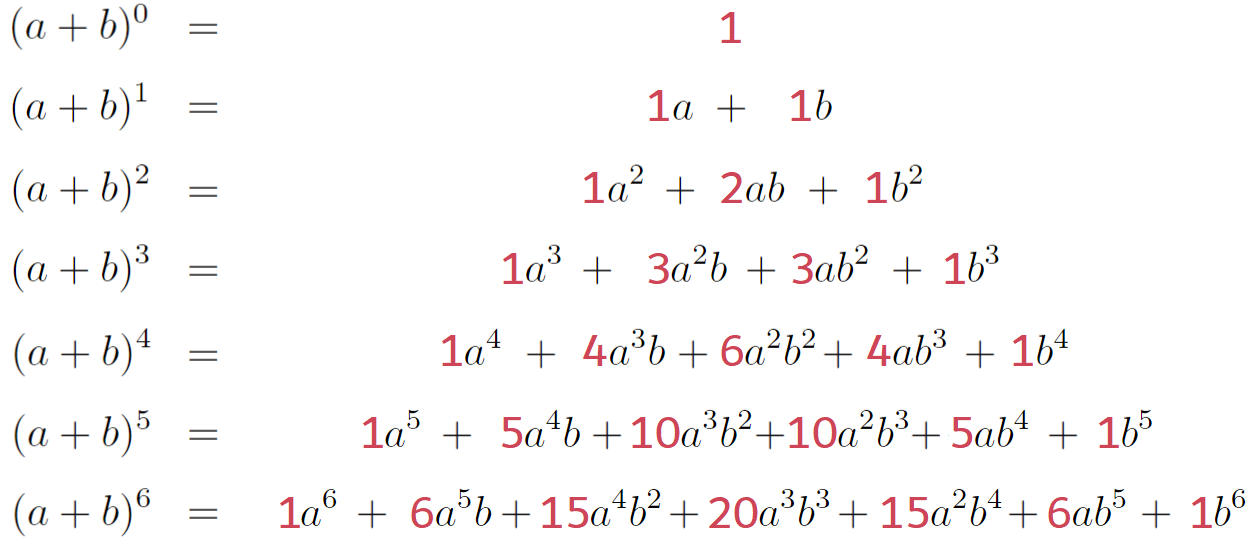
\includegraphics[width=0.72\textwidth]{二项式1.png}
\end{figure}

可以看到,每一行相邻的两个系数之和,等于下一行位于它们“中间”的数。
例如,第$5$行左起第$2$个数是$4$,第$3$个数是$6$。它们的和等于$10$,也就是第$6$行左起第$3$个数。

继续算出$n=7,8$时$(a+b)^n$的系数,可以验证,以上规律仍然成立。

公元$1261$年,南宋数学家杨辉所著的《详解九章算术》中就出现了这个三角数阵,
我们把它称为\textbf{杨辉三角形}。使用杨辉三角形,我们可以方便地查出$(a+b)^n$各项的系数。
下面我们归纳法证明以上规律。

记$(a+b)^n = \sum_{k=0}^n w_{k,n} a^k b^{n-k}$,其中$w_{k,n}$是各项系数。
设立命题$P(n)$:
$$P(n): \quad w_{0,n}=w_{n,n}=1, \quad \forall k\in[1\ldots n-1], \,\,\,\, w_{k,n} = w_{k,n-1} + w_{k-1,n-1}.$$

$n=2$时,$w_{1,2} = 2 = 1 + 1 = w_{1,1} + w_{0,1}$。因此$P(2)$为真。

若$P(n)$对某个自然数$n\geqslant 2$为真,根据归纳假设,
\begin{align}
 (a+b)^{n+1} &= (a+b)\cdot(a+b)^n = (a+b)\cdot\left(\sum_{k=0}^n w_{k,n} a^k b^{n-k}\right) \notag \\
  &= \sum_{k=0}^n w_{k,n} a^{k+1} b^{n-k} + \sum_{k=0}^n w_{k,n} a^k b^{n-k+1} \notag \\
  &= w_{n,n}a^{n+1} + \sum_{k=0}^{n-1} w_{k,n} a^{k+1} b^{n-k} + \sum_{k=1}^n w_{k,n} a^k b^{n-k+1} + w_{0,n}b^{n+1} \notag \\
  &= a^{n+1} + \sum_{k=1}^{n} w_{k-1,n} a^{k} b^{n-k+1} + \sum_{k=1}^n w_{k,n} a^k b^{n-k+1} + b^{n+1}\notag \\
  &= a^{n+1} + \sum_{k=1}^{n} (w_{k-1,n} + w_{k,n}) a^{k} b^{n-k+1} + b^{n+1} \notag
\end{align}
因此$w_{0,n+1}=w_{n+1,n+1}=1$;$\forall k\in[1\ldots n]$,$w_{k,n+1} = w_{k,n} + w_{k-1,n}$。
于是$P(n+1)$为真。因此,对任何为真大于等于$2$的自然数,$P(n)$为真。

根据以上递推公式,我们可以算出杨辉三角形任一行的数。以此为系数,我们可以写出任何$(a+b)^n$的展开式。

\section{二项式定理}

设$n=100$,我们想知道$(a+b)^n$的展开式。仅仅根据递推公式,为了算出$(a+b)^n$,
我们要先推出前$100$行。这样的计算太繁琐了。我们希望对每个系数有直接了解。能否有计算指定系数的“通项公式”?

我们先从比较小的$n$开始找规律。展开$(a+b)^2$的时候,我们根据分配律,得到
$$ (a+b)^2 = a\cdot a + b\cdot a + a\cdot b + b\cdot b. $$
然后把$ab$和$ba$合并同类项。展开$(a+b)^3$的时候,我们根据分配律,得到
\begin{align}
 (a+b)^3 &= a\cdot a\cdot a + b\cdot a\cdot a + a\cdot b\cdot a + b\cdot b\cdot a\notag \\
  &+ a\cdot a\cdot b + b\cdot a\cdot b + a\cdot b\cdot b + b\cdot b\cdot b \notag 
\end{align}
然后把$baa$、$aba$、$aab$合并同类项,得到$3a^2b$;把$bba$、$bab$、$abb$合并同类项,得到$3ab^2$。

一般来说,展开$(a+b)^n$时,我们已经知道所有的项都是$a^kb^{n-k}$乘以相应系数的形式,
其中的$a$和$b$来自于每次使用分配律时选择$a$还是$b$,而系数是所有相应选择的方法数。
具体来说,我们可以认为,展开$(a+b)^n$时,我们从$n$个连乘的$a+b$中不断选择,
把$n$次选择的结果乘起来,然后合并到某个$a^kb^{n-k}$中,成为它的系数中的“$1$”。
所有的“$1$”加起来,就变成了展开式中$a^kb^{n-k}$的系数。

例如,展开$(a+b)^6$时,我们已经知道有$a^2b^4$这一项($k=2$)。它的系数是在$6$个$a,b$中选择$2$次$a$、$4$次$b$的方法数,即组合数$C_6^2$。
于是,$(a+b)^6$的展开式中,$a^2b^4$这一项的系数是$C_6^2 = 15$。

对特定的$k$来说,$a^kb^{n-k}$的系数来自于我们展开时选择了$k$次$a$、$n-k$次$b$。
因此,$a^kb^{n-k}$的系数就等于选出$k$个$a$和$n-k$个$b$的方法数。它等于组合数$C_n^k$。
也就是说,$(a+b)^n$的展开式中,$a^kb^{n-k}$的系数为$C_n^k$。这个系数叫做\textbf{二项式系数}。
我们可以完整地写出$(a+b)^n$的展开式:
$$(a+b)^n = \sum_{k=0}^n C_n^k a^kb^{n-k} = \sum_{k=0}^n \frac{n!a^kb^{n-k}}{k!(n-k)!} .$$
这个结论称为\textbf{二项式定理},右边的式子称为$n$次二项展开式。其中为了方便,
约定$C_n^0 = \frac{n!}{0!n!} = 1 = C_n^n$。

组合数是二项式展开中的系数,因此,可以用二项式定理反过来推导出组合数的一些基本性质。
比如,由前面的结论可知:
$$C_n^k = C_n^{n-k}, \quad C_{n+1}^k = C_n^k + C_n^{k-1}.$$
又如,令$a=b=1$,可得到:
$$\sum_{k=0}^n C_n^k = 2^n.$$
令$a=-1$、$b=1$,可得到:
$$\sum_{k=0}^n (-1)^k C_n^k = 0.$$

观察杨辉三角形,还可以发现二项式系数的性质:从$C_n^0=1$起,随着$k$增大,
$C_n^k$先是不断增大,然后不断减小,最终回到$C_n^n = 1$。
$n=2m+1$为奇数的时候,$C_n^m=C_n^{m+1}$是数值最大的;$n=2m$为偶数时,
$C_n^m$是数值最大的。这些性质可以用以下关系式解释:
$$ C_n^k = \frac{n!}{k!(n-k)!} = \frac{n-k+1}{k}\cdot \frac{n!}{(k-1)!(n-k+1)!} = \frac{n-k+1}{k}C_n^{k-1}.$$
$k < n-k+1$的时候,$C_n^k > C_n^{k-1}$;$k > n-k+1$的时候,$C_n^k < C_n^{k-1}$。分水岭是$\frac{n+1}{2}$。

具体来说,$C_n^k$大概有多大呢?我们知道,使得$C_{n}^k$最大的$k$在$n$的一半左右。
使用渐进估计(需要用到较高深的知识,这里不展开介绍)可以知道,
$n$足够大之后,这个系数大致等于$\frac{2^{n}}{\sqrt{2\pi n}}$。
也就是说,所有二项式系数之和大致是最大的二项式系数的$2.5\sqrt{n}$倍。
二次项系数从$1$变成$n$,再变成$\frac{n(n-1)}{2}$,增长越来越慢,
最终在$n$的一半左右达到最大值————大约是$\frac{2^{n}}{\sqrt{2\pi n}}$,然后逐渐变小,最后回到$1$。

\begin{xt}
    \mbox{} \\
    \indent 1. 展开以下二项式:\\
    \indent 1.1. $(a+b)^8$、$(a-b)^{10}$ \\
    \indent 1.2. $(x+1)^7$、$(1-\frac{1}{x})^9$、$(x^2-\frac{1}{x})^5$ \\
    \indent 2. 观察$(1+x)^{2n}$的系数,证明:$\sum_{k=0}^n \left(C_n^k\right)^2 = C_{2n}^n.$ \\
    \indent 3. 观察$a^n = (a-b+b)^n$的系数,证明:
                $$\forall \,\, 0 \leqslant m < n, \,\,\, \sum_{k=m}^n (-1)^{k-m} C_n^kC_k^m = 0.$$
    \indent 4. $7^{103}$模$25$的余数是多少?

\end{xt}

\section{二项式的应用}

二项式在科学研究、生产生活中经常出现,有大量应用。这里举几个简单的例子。

\subsection{微扰估计}
\begin{et}
某酒厂培养的酵母在某种环境下每$6$个小时数量增加$1\%$。设初始培养基数为$100$个单位。$20$天后,该环境下的酵母数量能否超过$200$个单位?
\end{et}
\begin{so}  
    从已知条件出发,我们以$6$个小时为时间单位,估计酵母数量的增加情况。设初始时刻为$0$,初始时刻酵母数量为$A = 100$,把$6$个小时记为$t$,经过的时间单位个数为$n$。
    则在$t$时刻,酵母数量为$A(1 + d)$,其中$d=1\%$为单位时间增量的比例。再过$6$小时,在$2t$时刻,酵母数量为$A(1 + d)(1 + d) = A(1 + d)^2$。以此类推,
    在$nt$时刻,酵母数量为$A(1 + d)^n$。把每次经过单位时间后估计的酵母数量排列起来,得到一个等比数列,公比为$1 + d$。

    我们要估计的是$20$天后的酵母数量。每天有$24$个小时,因此$20$天相当于$n=80$个时间单位,于是我们估计$20$天后的酵母数量为$A(1 + 1\%)^{80}$。
    我们要判断$A(1 + 1\%)^{80}$是否大于$2A$,即$(1 + 1\%)^{80}$是否大于$2$。

    不使用电子设备直接计算$(1 + 1\%)^80$比较繁琐。我们用二项式定理来估计$(1 + 1\%)^{80}$。为了方便,我们采用$(1 + d)^n$的记法。
    根据二项式定理:
    $$(1 + d)^n = 1 + C_n^1 d + C_n^2 d^2 + \cdots + C_n^n d^n.$$
    
    上式右侧每一项都大于零。因此,只要其中部分项的和大于$2$,$(1 + d)^n$就大于$2$。我们从$k$较小的几项开始,计算每一项的大小。
    \begin{align}
        C_n^1 d = 80 \times 0.01 &= 0.8 \notag \\
        C_n^2 d = \frac{80 \times 79}{2\times 1} \times 0.01^2 &= 0.316 \notag \\ 
        C_n^3 d = \frac{80 \times 79\times 78}{3\times 2\times 1}80 \times 0.01^3 &= 0.08216 \notag
    \end{align}
    根据第一项的值可知:$(1 + d)^n > 1 + C_n^1 d = 1.8$,类似地,根据前两项、前三项的值可知:$(1 + d)^n > 2.116$、$(1 + d)^n > 2.19816$。
    因此,只要根据二项式展开后的前两项来估计,就能知道$(1 + 1\%)^{80}$大于$2$。
    
    答:$20$天后,该环境下的酵母数量超过$200$个单位。
\end{so}

我们把这样的问题称为\textbf{微扰估计问题},即估计一个形如$(1+x)^n$的式子在$x$很接近$0$的时候的值。
其中$x$称为扰动项。

我们知道,$(1+x)^n$展开式中,$x$的$k+1$次项是$x$的$k$次项乘以$\frac{(n-k+1)x}{k}$。因此,当$nx<1$的时候,展开式中$x$次数高的项的绝对值,
会比$x$次数较低的项小得多。如果$|nx|$远小于$1$,那么$(1+x)^n$展开式的各项随着$x$次数增加,绝对值快速减小,$x$次数高的项相比于$x$次数低的项
,小得可以忽略。于是,微扰估计问题中,我们主要估计前几项的值对问题的影响。

下面是另一个微扰估计的例子。

\subsection{近似计算}
\begin{et}
    已知某合金的长度热膨胀满足半经验公式:$l = l_0(1+\eta\frac{T-T_0}{T_0})^5$,
    原材料长度$l_0=25$厘米,系数$\eta=0.5$。当温度$T$从$T_0=650K$升到$654K$的时候,材料长度增加了多少厘米?将误差保持在$1\%$以内。
\end{et}
\begin{so}
    关键在于计算$(1+\eta\frac{T-T_0}{T_0})^5$。$\eta\frac{T-T_0}{T_0} = \frac{2}{650} \approx 0.00308$。
    因此需要计算
    $$ 1 + 5\cdot 0.00308 + 10\cdot 0.00308^2 + 10 \cdot 0.00308^3 + 5 \cdot 0.00308^4 + 0.00308^5. $$
    我们注意到$0.00308$是一个很小的数,它的平方、立方……只会迅速变得非常非常小。而二项式系数最大不超过$10$,
    因此,上式左起第$3$项开始相对前两项非常小。\\
    由于$5 \cdot 0.00308 = 0.0154$,而$10\cdot 0.00308^2 \approx 0.00009$,
    大概是$0.0154$的千分之六,在$1\%$以内,因此它之后的项就可以忽略了。我们可以说
    $$ (1+\frac{T-T_0}{T_0})^5 \approx 1 + 5\cdot 0.00308 + 10\cdot 0.00308^2 = 1.0155 $$
    因此,升温后材料长度约为$25\cdot 1.0155 = 25.387$厘米,增加了$0.387$厘米。
    精确计算的结果是$0.38699\dots$厘米,可以看出误差在$1\%$以内,未造成额外误差。   
\end{so}

在这个例子里,$x\approx 0.003$,
$$C_5^2x^2 = \left(\frac{5-2+1}{2}x\right)\cdot C_5^1x^1$$
括号中的$\frac{5-2+1}{2}x$远小于$1$,因此$C_5^2x^2$远小于$C_5^1x^1$,
其后的$C_5^3x^3$、$C_5^4x^4$、$C_5^5x^5$更是如此。于是,我们可以根据精度要求,适当舍掉靠后的大部分项,
只保留靠前$x$次数较低的项,快速估计出近似值。

实践中,我们只保留前一到两项,精度不够时,再逐步尝试。比如先计算$1 + C_n^1x = 1 + nx$,
再计算$1 + C_n^1x + C_n^2x^2 = 1 + nx + \frac{n(n-1)}{2}x^2$。如果两者之差在精度要求的误差范围内,
就可以用后一个作为估计结果。
\begin{et}
    计算$(1 - 0.0082)^{14}$,相对误差在$1\%$以内。
\end{et}
\begin{so}
    $n=14$,$x=-0.0082$,计算$1 + nx$和$1 + nx + \frac{n(n-1)}{2}x^2$的值,分别得到$0.8852$和$0.8913$。两者之差为$0.0061$,小于$1\%$,因此认为精度已达到要求,取$0.8913$为估计结果。经验证,精确结果为$0.89112\dots$,相对误差在$1\%$以内。
\end{so}
\begin{et}
    计算$1.9926^{19}$,相对误差在$1\%$以内。
\end{et}
\begin{so}
    将问题转化为求$2^{19}\cdot(1-\frac{2-1.9926}{2})^{19}$。这时$n=19$,$x = -\frac{2-1.9926}{2} = -0.0037$。计算$1 + nx$和$1 + nx + \frac{n(n-1)}{2}x^2$的值,分别得到$0.9297$和$0.9320$。两者之差为$0.0023$,小于$1\%$,因此认为精度已达到要求。估计结果为$2^{19}\cdot 0.9320=488636.416$。经验证,精确结果为$488632.549\dots$,相对误差在$1\%$以内。
\end{so}

\begin{sk}
    如果某合金的长度热膨胀满足半经验公式:$l = l_0(1+\eta\frac{T-T_0}{T_0})^{0.5}$。原材料长度$l_0=25$厘米,系数$\eta=0.5$。当温度从$400K$升到$450K$时,材料长度如何变化?
\end{sk}

\begin{xt}
    \mbox{} \\
    \indent 1. 设有正整数$n > 1$,实数$x > 0$,证明:$(1 + x)^n > 1 + nx.$\\
    \indent 2. 设有正整数$n > 1$,实数$x > -1$且$x \neq 0$,用归纳法证明:$(1 + x)^n > 1 + nx.$
\end{xt}

\subsection{二项分布}

我们已经学习过单一实验中的二项分布。比如,抛一枚硬币,硬币正面向上的概率是$p$,
向下的概率是$1-p$,就说实验结果服从系数为$p$的二项分布。现在来看独立重复这个实验的分布。

假设重复抛掷$n$次硬币,任何两次之间互不干扰。这个独立重复实验中,每次抛掷正面向上的概率为$p$,
向下的概率为$1-p$。$n$次抛掷是相互独立的,因此,某$k$次抛掷正面向上,其余$n-k$次抛掷向下的概率是$p^k(1-p)^{n-k}$。
$n$次抛掷中,要使得$k$次抛掷向上,有$C_n^k$种可能,因此,$n$次抛掷中有$k$次正面向上的概率就是$C_n^kp^k(1-p)^{n-k}$,
也就是二项式$(p + 1-p)^n$展开中第$k+1$项。这样的分布称为系数为$p$的$n$次二项分布。
$n$次抛掷的终态有$n+1$个,其分布列为:
\begin{center}
    \begin{tabular}{| p{4em}<{\centering} | p{8em}<{\centering} |}
        \hline
        $\mathbf{k}$ & $\mathbb{P}(\mathbf{k}\mbox{\textbf{次正面向上}})$ \\ [0.5ex] 
        \hline
        $0$ & $C_n^0 p^0(1 - p)^n\quad$ \\  
        \hline
        $1$ & $C_n^1 p^1(1 - p)^{n-1}\,$ \\  
        \hline
        $\vdots$ & $\vdots$  \\    [0.75ex] 
        \hline
        $n-1$ & $C_n^n p^{n-1}(1 - p)^{1}\quad$ \\ 
        \hline
        $n$ & $C_n^n p^n(1 - p)^{0}\quad$ \\ 
        \hline
    \end{tabular}
\end{center}
比如,抛掷$n=20$次硬币,向上概率为$p=0.4$的时候,分布可以用以下直方图表示:

\begin{figure}[h]
    \vspace{4pt}
    \centering
    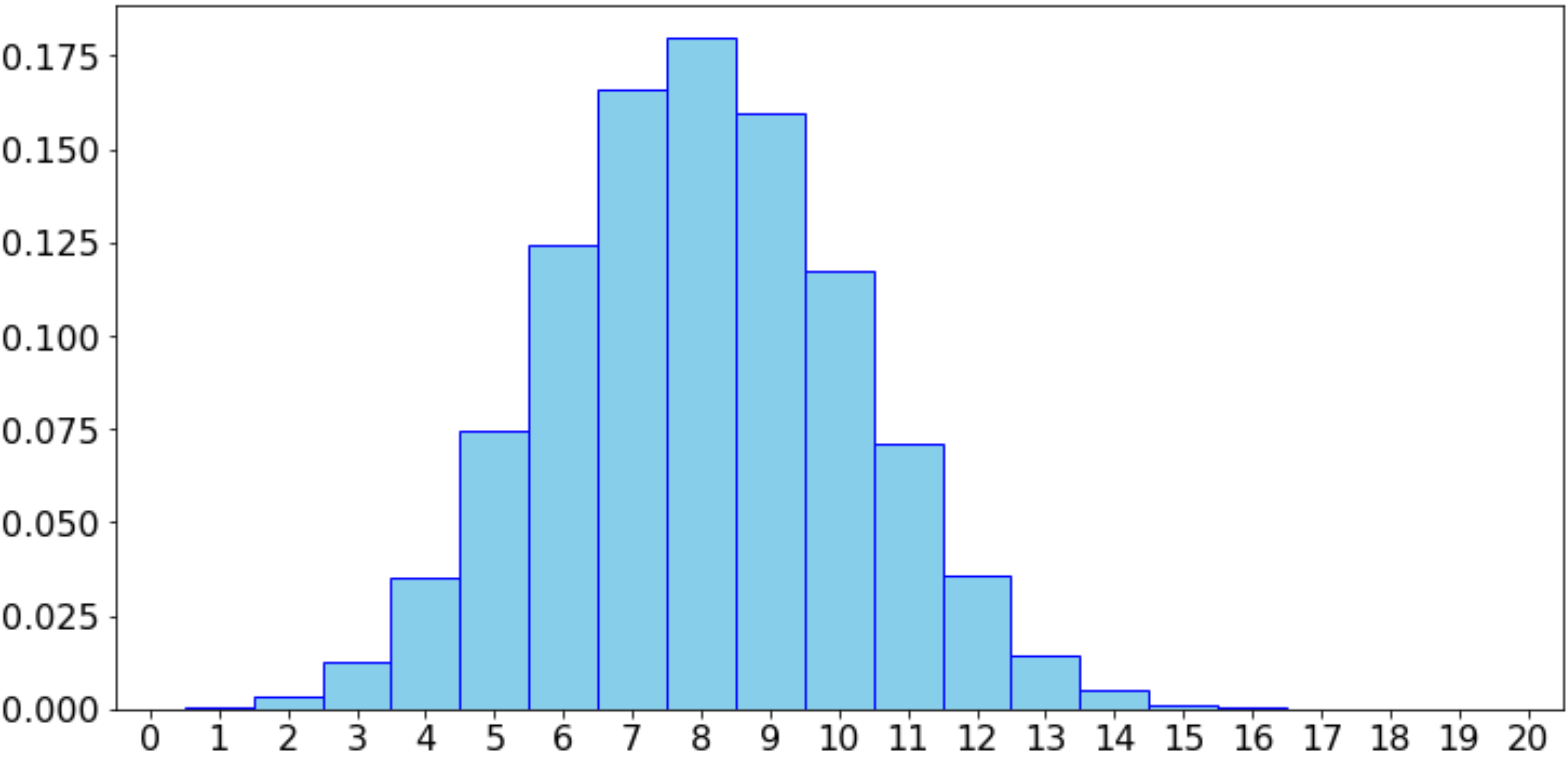
\includegraphics[width=0.96\textwidth]{二项分布直方图.png}
    \caption*{\texttt{二项分布的直方图(}$n=20,\,\,\, p=0.4$\texttt{)}}
\end{figure}

可以算出,$5$次向上的概率约为$0.0746$,$10$次向上的概率约为$0.1171$,$15$次向上的概率约为$0.0013$。

\begin{xt}
    \mbox{} \\
    独立重复抛掷$15$次硬币,每次抛掷向上的概率是$0.6$。\\
    \indent 1. 计算:$3$次向上、$6$次向上、$8$次向上的概率分别是多少?\\
    \indent 2. 画出这个实验结果的分布列。\\
    \indent 3. 几次向上的概率最大?
\end{xt}

\chapter{实变函数中的极限}
我们已经学习了数列的极限。数列是正整数集上的映射。下面我们将继续研究实变函数。
数列的极限,对研究实数集上的函数,有什么作用呢?

考虑以下映射:
\begin{align}
    f_{\mathbb{Q}}: \mathbb{Q} &\rightarrow \mathbb{R}\notag \\
    x &\mapsto 2^x \notag
\end{align}
$f_{\mathbb{Q}}$定义在有理数域$\mathbb{Q}$上,把一个数$x$映射到$2$的$x$次幂。
当$x$是有理数时,我们能够定义“$2$的$x$次幂”。
当$x$不是有理数的时候,我们能不能合理地定义“$2$的$x$次幂”呢?换句话说,是否有一个比较好的实变函数$f_{\mathbb{R}}$,
当$x$是有理数时,$f_{\mathbb{R}}(x) = f_{\mathbb{Q}}(x)$呢?

首先,我们要明确定义:当我们说“比较好”的时候,我们指的是什么。如果$x$不是有理数的时候,$f_{\mathbb{R}}(x) = 0$,
那么我们说这样的函数$f_{\mathbb{R}}$不够好。为什么呢?让我们画出这个函数的图像。一般来说,要画一个实变函数,
我们会用“描点连线”的办法,先求出函数在一系列点上的值,然后用直线把相邻的点连起来。我们认为,这样得到的图像,和函数的真实图像大致一样。

比如,我们想画出函数$f_{\mathbb{R}}$在区间$[1.4,\,\,1.5]$上的图像。我们发现,$f_{\mathbb{R}}(1.4)$和$f_{\mathbb{R}}(1.5)$
都大于2,乃至$f_{\mathbb{R}}(1.41)$、$f_{\mathbb{R}}(1.42)$、$f_{\mathbb{R}}(1.415)$都大于$2$,但$f_{\mathbb{R}}(\sqrt{2}) = 0$!
这说明$x$的值产生微小变化的时候,函数的值会有突然的“跳跃”。这样,我们无法凭直觉用“描点连线”的办法来理解这个函数了。因此,我们希望
$f_{\mathbb{R}}(\sqrt{2})$最好和$f_{\mathbb{R}}(1.41)$、$f_{\mathbb{R}}(1.42)$差不多大,让我们从$1.4$画到$1.5$的时候,函数的值不会突然“跳跃”。

另一方面,不难发现,$f_{\mathbb{Q}}$自身有不少基本性质。比如,$f_{\mathbb{Q}}$是单调递增函数。此外,它有这样的性质:
$$\forall \, a, b\in \mathbb{Q}, \,\,\, f_{\mathbb{Q}}(a) \cdot f_{\mathbb{Q}}(b) = f_{\mathbb{Q}}(a + b).$$
我们希望$f_{\mathbb{R}}$对任意实数也保持这样的性质。这时,让$f_{\mathbb{R}}$在无理数上的取值为$0$显然也是不行的。

到底什么样的函数是比较好的?我们发现,用四则运算、乘方开方、大小关系,都没法准确描述我们想要的性质。
上一章中,我们知道了实数可以用有理数列的极限来表示。
因此,下面我们尝试用数列的极限来描述我们直觉中“比较好”的函数。

\section{实变函数在一点的极限}
我们知道,给定实数$x$,存在有理数列$\{x_n\}_{n\in\mathbb{Z}^+}$趋于$x$。
考虑数列$\{f_{\mathbb{Q}}(x_n)\}_{n\in\mathbb{Z}^+}$,它是否有极限呢?

我们从一个特殊的点开始研究。
\begin{et}
    考虑$x=0$,对任意一个趋于$0$的有理数列$\{x_n\}_{n\in\mathbb{Z}^+}$,考察数列$\{2^{x_n}\}_{n\in\mathbb{Z}^+}$。它是否有极限?
\end{et}
\begin{so}
    从简单的数列开始研究。考虑数列$\{2^\frac{1}{n}\}_{n\in\mathbb{Z}^+}$,它是否有极限?

    设$a_n = 2^\frac{1}{n}$,则$a_n^n = 2$。我们知道,对给定的正整数$n$,$x>0$时,$x\mapsto x^n$是递增函数。$1^n=1$,$2^n\geqslant 2$,所以总有$1<a_n\leqslant 2$。
    另一方面,$x>1$固定时,$x^\frac{1}{n}$随着$n$增大而减小,所以$a_n$随着$n$增大减小,向$1$接近。

    到底$a_n$和$1$多接近呢?我们来计算$\left(1+\frac{1}{n}\right)^n$。

    根据二项式定理:
    \begin{align}
        \left(1+\frac{1}{n}\right)^n &= 1 + C_n^1\cdot \frac{1}{n} + C_n^2\cdot \left(\frac{1}{n}\right)^2 + \cdots + C_n^n\cdot \left(\frac{1}{n}\right)^n \notag \\
        &> 1 + C_n^1\cdot \frac{1}{n} = 1 + \frac{n}{n} = 2. \notag
    \end{align}
    这说明$1<a_n\leqslant 1 + \frac{1}{n}$。对任意$r>0$,总有正整数$N$使得只要$n>N$时,$\frac{1}{n}<r$,于是$0 < a_n - 1 < \frac{1}{n} < r$。
    这说明数列$\{2^\frac{1}{n}\}_{n\in\mathbb{Z}^+}$收敛到$1$。

    对于其他趋于$0$的有理数列$\{x_n\}_{n\in\mathbb{Z}^+}$,$\{2^{x_n}\}_{n\in\mathbb{Z}^+}$是否也趋于$1$呢?我们可以拿它和$\{a_n\}$作比较。

    按照定义,对任何正整数$N$,由于$\frac{1}{N}>0$,存在正整数$n$,使得$m>n$时总有$|x_m| < \frac{1}{N}$,即$2^{-\frac{1}{N}} < 2^{x_m} < 2^\frac{1}{N}$。
    因此,对任意$r>0$,我们可以先找到正整数$N_+$,使得$2^{\frac{1}{N_+}} < 1 + r$,然后再根据$N_+$找到正整数$n_+$,使得$m>n_+$时$2^{x_m} < 2^\frac{1}{N_+}$,即
    $2^{x_m} < 1 + r$。

    这只是$\{2^{x_n}\}_{n\in\mathbb{Z}^+}$趋于$1$的“一半”条件。当然,另一边也可以类比处理。$\{2^{-\frac{1}{n}}\}_{n\in\mathbb{Z}^+}$收敛到$1$的倒数,仍然是$1$。
    因此可以找到正整数$N_-$,使得$1 - r < 2^{\frac{1}{N_-}}$,然后再根据$N_-$找到正整数$n_-$,使得$m>n_-$时$2^{-\frac{1}{N_-}} < 2^{x_m}$,即
    $1 - r < 2^{x_m}$。
    
    综上,取正整数$n$为$n_-,n_+$中较大者,那么$m>n$时就总有$\left|2^{x_m} - 1\right| < r$。于是$\{2^{x_n}\}_{n\in\mathbb{Z}^+}$趋于$1$。
\end{so}

从直观上看,这说明$f_{\mathbb{Q}}$在平面中的曲线在点$(0,\,\,1)$附近没有“突变”或“跳跃”。无论自变量$x$以什么方式靠近$0$,$f_{\mathbb{Q}}(x)$都随之靠近$1$。
不会出现突然的变动。这符合我们对$f_{\mathbb{Q}}$曲线的大致印象。

一般来说,我们把$1$称为函数$f_{\mathbb{Q}}$在(数轴上)$0$这一点的极限。
\begin{df}\textbf{实变函数在一点的极限}
    给定实数$a$和实变函数$f$,如果对任何趋于$a$的数列$\{a_n\}_{n\in\mathbb{Z}^+}$,数列$\{f(a_n)\}_{n\in\mathbb{Z}^+}$只要可定义
    ($a_n$总在$f$定义域中),就趋于同一个极限$b$,那么就说$b$是函数$f$在$a$处的\textbf{极限},
    也可以说自变量趋于$a$时,$f$趋于或\textbf{收敛到}$b$,记作:
    $$  \lian{x \to a} f(x) = b. $$
\end{df}

从定义可以看出,我们不要求$f$在$a$处有定义。

可以证明,函数在一点如果有极限,则极限是唯一的。因此,我们也说$f$在$a$处的极限是$b$。

函数$f_{\mathbb{Q}}$在$0$处的极限是它在$0$处的函数值,这是一个很重要的性质。
从这个结论出发,我们可以考虑$f_{\mathbb{Q}}$在任意有理数$a$处的极限。

考虑收敛到$a$的有理数列$\{a_n\}$,数列$\{a_n - a\}$收敛到$0$。因此,按以上结论,$\{f_{\mathbb{Q}}(a_n - a)\}$收敛到$1$。
但我们可以算出,
$$f_{\mathbb{Q}}(a_n - a) = 2^{a_n - a} = \frac{2^{a_n}}{2^a}. $$
这说明数列$\{2^{a_n}\}$趋于$2^a$,即$f_{\mathbb{Q}}(a)$。这说明$f_{\mathbb{Q}}$在任一点的极限都是该点的函数值。
我们将在后文讨论这个性质。

让我们再来看一个简单的例子。
\begin{et}
    求函数$f:x\mapsto x^2$在$x=0$处的极限。
\end{et}
\begin{so}
    按照定义,我们考虑任意一个趋于$0$的数列$\{x_n\}_{n\in\mathbb{Z}^+}$。按照极限的运算法则,数列$\{x_n^2\}_{n\in\mathbb{Z}^+}$也趋于$0$。
    这个性质对任何趋于$0$的数列成立。这说明$0$是函数$f$在$0$处的极限。
\end{so}

直观上,函数在一点的极限,就是画函数图像时,曲线“应该经过”的地方。
具体来说,如果函数$f$在实数$a$处有极限$b$,那么当$f$图像上一点$x$的横坐标与$a$足够接近时,
它的纵坐标应该和$b$足够接近。最终,函数图像“应该经过”点$(a,\,\, b)$。
这种说法并不严谨,但可以给我们一点直觉上的帮助。

数列除了趋于某个极限,还可能趋于正负无穷大。对应地,函数在一点也有类似的性质。
\begin{df}
    给定实数$a$和实变函数$f$,如果对任何趋于$a$的数列$\{a_n\}_{n\in\mathbb{Z}^+}$,数列$\{f_{\mathbb{Q}}(a_n)\}_{n\in\mathbb{Z}^+}$只要可定义
    ($a_n$总在$f$定义域中),就趋于正(负)无穷大,那么就说$b$是函数$f$在$a$处趋于正(负)无穷大。
    也可以说自变量趋于$a$时,$f$趋于趋于正(负)无穷大。记作:
    $$  \lian{x \to a} f(x) = \pm\infty. $$
\end{df}

\begin{et}
    计算函数$f: x\mapsto \frac{1}{x^2}$在$0$处的极限。
\end{et}
\begin{so}
    考虑任意趋于$0$的数列$\{x_n\}$。为了让$f(x_n)$有定义,$x_n$不为$0$。按照定义,对任意正数$A$,由于$\frac{1}{\sqrt{A}} > 0$,
    总能找到正整数$N$,使得$n>N$时总有$|x_n| < \frac{1}{\sqrt{A}}$,也就是说$f(x_n) = \frac{1}{x_n^2} > A$。这说明$f$在$0$处趋于正无穷大。
\end{so}

最后我们来介绍函数在一点极限的另一种表述。这种表述不再使用数列的概念,而使用区间的概念。

\begin{df}\textbf{实变函数在一点的极限}
    给定实数$a$、$b$和实变函数$f$。如果对任何$r>0$,都存在$d>0$,
    使得开区间$(a-d,\,\,a+d)$中的数$x$经过$f$得到的函数值$f(x)$
    总在开区间$(b-r,\,\,b+r)$中\footnotemark:
    $$ |b - f(x)| < r,$$
    就说$b$是函数$f$在自变量等于$a$时的\textbf{极限}。也可以说自变量趋于$a$时,$f$趋于或\textbf{收敛到} $b$。
\end{df}
\footnotetext{与前一种定义里一样,这里的前提是$f(x)$可定义。}

我们把$(a-d,\,\,a+d)$这样的区间称为$a$的$d$–\textbf{邻区间}。它可以描述“与$a$邻近”的概念。

用邻区间定义函数在一点的极限,更加简明方便。它的形式与数列极限的定义比较像。我们不需要讨论所有趋近点$a$的数列,
而是从任意正数$r$出发,说明总能找到某个数$d$,满足相关条件。

下面用邻区间定义来证明$f:x\mapsto x^2$在$x=0$处的极限是$0$。
\begin{proof}
    任意给定正数$r$,取$d = \sqrt{r}$,那么
    $x$在邻区间$U(0,\,\, d)$中的时候,总有$|x| < d$,于是:
    $$f(x) = x^2 < d^2 = r.$$
    这说明$f$在$x=0$处的极限是$0$。
\end{proof}

用邻区间定义的极限和数列定义是等价的,最后我们来证明这一点。
\begin{proof}
    给定实数$a$、$b$和实变函数$f$。

    首先证明数列定义的极限可以推出邻区间定义的极限:如果对任意趋于$a$的数列$\{a_n\}$,$\{f(a_n)\}$都趋于$b$,
    那么对于任意正数$r$,都存在正数$d$,使得对任何$x\in U(a,\,\, d)$,总有$f(x)\in U(b,\,\,r)$。

    使用反证法来证明。反设有正数$r$,使得上述的$d$不存在。那么,对任何$d>0$,总有某个$x_d\in U(a,\,\, d)$,
    使得$ |b - f(x_d)| \geqslant r$。我们取一组特殊的$d$,比如$d = \frac{1}{n}$,对应的$x_d$记作$x_n$,就得到一个数列:$\{x_n\}$。
    
    按照数列$\{x_n\}$的定义,它趋于$a$。另一方面,$f(x_n)$与$b$的差总大于$r$。因此,数列$\{f(x_n)\}$不趋于$b$。这与数列定义矛盾。
    因此原命题成立。数列定义的极限可以推出邻区间定义的极限。

    再证明邻区间定义的极限可以推出数列定义的极限:如果对于任意正数$r$,都存在正数$d$,使得对任何$x\in U(a,\,\, d)$,总有$f(x)\in U(b,\,\,r)$,
    那么,对任意趋于$a$的数列$\{a_n\}$,$\{f(a_n)\}$都趋于$b$。

    对任一个趋于$a$的数列$\{a_n\}$,我们要证明$\{f(a_n)\}$趋于$b$。给定正数$r$,我们需要找到正整数$N$,
    使得$n>N$时总有$|f(a_n) - b| < r$,即$f(a_n)\in U(b,\,\,r)$。
    
    根据邻区间定义,存在正数$d$,使得对任何$x\in U(a,\,\, d)$,总有$f(x)\in U(b,\,\,r)$。
    因此,我们只需要让$n>N$时总有$a_n\in U(a,\,\, d)$。而由于$\{a_n\}$趋于$a$,对于正数$d$
    来说,存在正整数$N$,使得$n>N$时总有$|a_n - a| < d$,也就是说$a_n\in U(a,\,\, d)$。
    于是这个$N$就是我们要找的正整数:$n>N$时总有$f(a_n)\in U(b,\,\,r)$。
    这就证明了,邻区间定义的极限可以推出数列定义的极限。

\end{proof}

\begin{sk}
    \mbox{} \\
    \indent 1. 考虑实变函数$f$和实数$a$。实数$d$大于$0$。设$f$在区间$\overset{\circ}{U}(a,\,\,d) = (a-d,\,\,a)\cup (a,\,\,a+d)$(也称为$a$的$d$–\textbf{去心邻区间})上有定义。试用邻区间的概念给出“函数$f$在$a$处趋于正(负)无穷大”的定义。\\
    \indent 2. 考虑实数$a$和实变函数$f, g$。设$f$在$a$的某个去心邻区间$\overset{\circ}{U}(a,\,\,d)$上有定义,且$f$在$a$处极限为$b$。若$g$在$b$的某个去心邻区间$\overset{\circ}{U}(b,\,\,d')$上有定义,
    ,且$g$在$b$处极限为$v$,那么复合函数$g\circ f$是否在$a$处有极限?如果有极限,极限是多少?
\end{sk}

\begin{xt}
    \mbox{} \\
    \indent 1. 证明基本函数的极限:\\
    \indent 1.1. 设$c$为常数,则函数$x\mapsto c$在任一点的极限总是$c$。\\
    \indent 1.2. 恒等函数$x\mapsto x$在任一点$a$处的极限总是$a$。\\
    \indent 1.3. 设$c$为常数,如果函数$f$在一点$a$的极限是$b$,那么函数$x\mapsto cf(x)$在$a$处的极限是$bc$。\\
    \indent 2. 考虑实变函数$f$和实数$a, b$。我们定义函数$f$在$a$处的\textbf{左极限}:如果对任何$r>0$,都存在$d>0$,使得开区间$(a-d,\,\,a)$中的数$x$经过$f$得到的函数值$f(x)$总在开区间$(b-r,\,\,b+r)$中,
    就说$f$在$a$处的左极限是$b$。\\
    \indent 2.1. 参照左极限的定义,给出函数\textbf{右极限}的定义。\\
    \indent 2.2. 参照极限的数列定义,给出左极限和右极限的数列定义。\\
    \indent 2.3. 证明:函数$f$在$a$处有极限,当且仅当它在$a$处有左极限和右极限,且左极限等于右极限。\\
    \indent 2.4. 考虑绝对值函数:$f:x\mapsto |x|$。它在$0$处是否有极限?
\end{xt}

\section{函数与极限}
与数列极限一样,函数在一点的极限也可以进行运算。考虑函数$f,g$。设它们在某点$a$有极限,极限分别是$u, v$。按照定义,任意数列$\{a_n\}$趋于$a$时,
$\{f(a_n)\}$趋于$u$,$\{g(a_n)\}$趋于$u$,因此$\{f(a_n) + g(a_n)\}$趋于$u + v$。这说明$f + g$在$a$处有极限,极限是$u + v$。同理,
$f - g$在$a$处有极限,极限是$u - v$;$f \cdot g$在$a$处有极限,极限是$u \cdot v$。$v\neq 0$时,$f\div g$在$a$处有极限,极限是$u \div v$。

我们可以把这些运算规则写成:
\begin{align}
    \lian{x \to a} (f + g)(x) = \lian{x \to a} f(x) + \lian{x \to a} g(x) \notag \\
    \lian{x \to a} (f - g)(x) = \lian{x \to a} f(x) - \lian{x \to a} g(x) \notag \\
    \lian{x \to a} (f \cdot g)(x) = \lian{x \to a} f(x) \cdot \lian{x \to a} g(x) \notag \\
    \lian{x \to a} (f \div g)(x) = \lian{x \to a} f(x) \div \lian{x \to a} g(x) \notag
\end{align}

函数在一点的极限可以进行关于函数的运算。这对我们计算复杂函数在一点的极限很有帮助。

\begin{et}
    求函数$f:x\mapsto x^2$在$x=0$处的极限。
\end{et}
\begin{so}
    定义恒等函数$h: x\mapsto x$,则$f = h \cdot h$。因此,$f$在$0$处的极限,是$h$在$0$处极限的平方。恒等函数$h$在$0$处的极限显然是$0$。
    所以,$f$在$0$处的极限等于$0$的平方,也就是$0$。
\end{so}

数列的极限是数列的项接近“无穷远”时的大体行为。这让我们思考,函数是否也有这样的大体行为。对于定义域允许的函数,
除了在一点的极限,我们可以考虑它在“无穷远”时的大体行为。

\begin{df}{\textbf{函数在无穷远处的极限}}
    设有实变函数$f$和实数$a$。$f$对任意大的实数有定义。如果对任何趋于正无穷大的数列$\{x_n\}$,$f(x_n)$都趋于$a$,就说$a$是$f$在正无穷远处的极限,
    记为:
    $$ \lian{x\to +\infty} f(x) = a$$
    如果对任何趋于正无穷大的数列$\{x_n\}$,$f(x_n)$都趋于正(负)无穷大,就说$f$在正无穷远处趋于正(负)无穷大,记为:
    $$ \lian{x\to +\infty} f(x) = \pm\infty$$
    同理,设$f$对任意小的实数有定义。如果对任何趋于负无穷大的数列$\{x_n\}$,$f(x_n)$都趋于$a$,就说$a$是$f$在正无穷远处的极限,记为:
    $$ \lian{x\to -\infty} f(x) = a$$
    如果对任何趋于负无穷大的数列$\{x_n\}$,$f(x_n)$都趋于正(负)无穷大,就说$f$在负无穷远处趋于正(负)无穷大,记为:
    $$ \lian{x\to -\infty} f(x) = \pm\infty$$
\end{df}

\begin{et}
    求函数$f:x\mapsto \frac{1}{x}$在无穷远处的极限。
\end{et}
\begin{so}
    考虑任何趋于正无穷大的数列$\{x_n\}$。按照定义,对任意$A>0$,都有正整数$N$,使得$n>N$时总有$x_n > A$。这说明$0 < \frac{1}{x_n} < A$。
    于是$f(x_n)$趋于$0$。因此$f$在正无穷远处的极限是$0$。同理,考虑任何趋于负无穷大的数列$\{x_n\}$。可以证明,$f(x_n)$趋于$0$。因此$f$在负无穷远处的极限是$0$。
\end{so}

\begin{et}
    求函数$f:x\mapsto x^2$在无穷远处的极限。
\end{et}
\begin{so}
    考虑任何趋于正无穷大的数列$\{x_n\}$。按照定义,对任意$A>0$,$A+1>0$,于是有正整数$N$,使得$n>N$时总有$x_n > A+1$。这说明$x_n^2 > (A+1)^2 > A$。
    于是$f(x_n)$趋于正无穷大。因此$f$在正无穷远处趋于正无穷大。同理,考虑任何趋于负无穷大的数列$\{x_n\}$。可以证明,$f(x_n)$趋于正无穷大。
    因此$f$在负无穷远处趋于正无穷大。
\end{so}

\begin{et}
    求函数$f:x\mapsto \frac{\sin{x}}{x}$在$0$处的极限。
\end{et}
\begin{so}
    我们已经证明过,任何(非零)数列$\{a_n\}$趋于$0$的时候,$\frac{\sin{a_n}}{a_n}$趋于$1$。
    因此,$f$在$0$处的极限是$1$。要注意的是$f$在$0$处没有定义。
    这么说来,只要定义$f(0) = 1$,那么$f$在$0$处的极限就等于它在$0$处的值。
\end{so}

\begin{sk}
    \mbox{} \\
    \indent 1. 用邻区间的极限定义,证明函数在一点的极限可以进行四则运算。\\
    \indent 2. 考虑在全体实数上有定义的函数$f$,及函数$g:x\mapsto f\left(\frac{1}{x}\right)$。$g$在$0$处的极限和$f$在无穷远处的极限有何联系?
    $f$在$0$处的极限和$g$在无穷远处的极限有何联系?
\end{sk}

\begin{xt}
    \mbox{} \\
    \indent 1. 计算以下极限。\\
    \indent 1.1. 函数$f:x\mapsto 2x - 1$在$x = -2$处的极限。\\
    \indent 1.2. 函数$f:x\mapsto 2x(1 - x)$在$x = 1$处的极限。\\
    \indent 1.3. 函数$f:x\mapsto \frac{x}{1 + x}$在$x = 0$处的极限。\\
    \indent 1.4. 函数$f:x\mapsto \frac{2^x}{x^2}$在$x = 0$处的极限。\\
    \indent 2. 设函数$f$和$g$对任意大的实数有定义。\\
    \indent 2.1. 证明:如果函数$f$和$g$在正无穷远处有极限$a, b$,则$f + g$、$f - g$、$f \times g$在正无穷远处也有极限,
    分别是$a + b$、$a - b$、$a \times b$。如果$b\neq 0$,那么$f \div g$在正无穷远处有极限$a \div b$。\\
    \indent 2.2. 证明:如果函数$f$和$g$在正无穷远处都趋于正无穷大,那么$f + g$、$f \times g$在正无穷远处也趋于正无穷大。
    如果$f$趋于正无穷大,$g$趋于负无穷大,那么$f - g$在正无穷远处趋于正无穷大、$f \times g$在正无穷远处趋于负无穷大。\\
    \indent 2.3. 如果函数$f$和$g$在正无穷远处都趋于负无穷大,那么$f + g$、$f \times g$在正无穷远处有何性质?\\
    \indent 3. 计算以下极限。\\
    \indent 3.1. 函数$f:x\mapsto 1 - \frac{1}{x}$在正无穷远处的极限。\\
    \indent 3.2. 函数$f:x\mapsto \frac{2 - 3x}{1 + x}$在负无穷远处的极限。\\
    \indent 3.3. 函数$f:x\mapsto \frac{x^2}{1 + x}$在无穷远处的极限。\\
    \indent 4. 考虑正弦函数$\sin$,它在无穷远处是否有极限?以此构造一个在$0$处没有极限的有界函数。
\end{xt}

\section{连续函数}

上一节中,我们提到$f_{\mathbb{Q}}$的一个性质:$f_{\mathbb{Q}}$在任一点的极限都是该点的函数值。我们把这样的性质称为\textbf{函数的连续性质}。

\begin{df}{\textbf{实变函数在一点连续}}
    设实变函数$f$在实数$a$及其某个邻区间上有定义。如果$f$在$a$处有极限,且极限等于$f(a)$,就说$f$在$a$处\textbf{连续}。
\end{df}

直观上来说,函数在一点连续,就是它经过它“应该经过”的地方,把函数图像在该点前后的部分“连上”了。
反之,如果函数在某处的值不是它在该处的极限,说明它没有经过“应该经过”的地方。
另一种可能是函数在该处没有极限,即无法确定“应该经过”什么地方。这时函数自然无法在该点连续了。

关于实变函数在一点连续的定义,要注意几点:
\begin{enumerate}
    \item 实变函数在一点的连续性质是一个\textbf{局部}的性质。具体来说,我们要求函数$f$在实数$a$及其某个邻区间上有定义。这个邻区间可以任意小。
    这说明,讨论函数在一点的连续性时,我们可以避开考虑函数在其他地方的性质。比如,我们要讨论$f$在$1$处是否连续,可以不考虑$f$在$1.001$处的性质,因为我们可以只考虑邻区间$(0.9999,\,\,1.0001)$。
    \item 实变函数在一点连续,要求它在该点有定义。这与函数在一点的极限有区别。函数“在一点连续”是比它“在一点有极限”更高的要求。
    \item 我们定义过函数在一点的左(右)极限。相应地,可以定义函数在一点\textbf{左}(\textbf{右})\textbf{连续}。这种定义对于定义域不是全体实数的函数很适用。
    比如,当我们讨论$f:x\mapsto \sqrt{x}$在$0$处是否连续时,可以说它右连续。
\end{enumerate}

\begin{et}
    考虑函数$f:x\mapsto x^2$,证明它在$x=0$处连续。
\end{et}
\begin{so}
    我们已经在上一节中计算了$f$在$0$处的极限。$f$在$0$处的极限是$0$,等于$f(0)$,所以,$f$在$0$处连续。
\end{so}

以上的思路可以用于任一点。所以我们可以更进一步:
\begin{et}
    证明函数$f:x\mapsto x^2$在任意实数$a$处连续。
\end{et}
\begin{so}
    对任意实数$a$,计算$f$在$a$处的极限。由极限关于函数的运算法则可知,$f$在$a$处的极限是$a^2$,等于$f(a)$。这说明$f$在任意实数$a$处连续。
\end{so}

我们证明了函数$f:x\mapsto x^2$在任意实数$a$处连续。这种连续性质不再是局部的,而是全局的。我们说$f$在实数集$\mathbb{R}$上连续。

一般来说,给定区间,如果函数$f$在区间中任一处连续,就说$f$在该区间\textbf{处处连续},或者说$f$是该区间上的\textbf{连续函数},该区间是$f$的\textbf{连续区间}。

对$f:x\mapsto x^2$来说,连续区间可以是全体实数构成的区间$(-\infty,\,\,\infty)$,也可以是$[1,\,\, 3]$这样的区间。

实变函数的连续性质是对生活中“连续的线”概念的抽象。如果函数在某个区间上连续,那么它的图像在直观上是一条连续不断的线,不会有“断点”。

用证明$f:x\mapsto x^2$连续的方法,我们可以证明,对于一般的一元整式$P$,函数$x\mapsto P(x)$是连续函数,在$\mathbb{R}$上连续。

再来看另一类基本的函数:三角函数。我们可以证明,正弦函数和余弦函数都是连续函数,在$\mathbb{R}$上连续。

首先证明正弦函数是连续函数。考虑任意实数$a$,我们证明正弦函数在$a$处连续。

按照定义,对任意正实数$r$,我们要证明存在$d>0$,使得只要
$x\in(a-d,\,\,a+d)$,就有$|\sin{x} - \sin{a}| < r$。

使用和差化积公式。
\begin{align}
    |\sin{x} - \sin{a}| &= \left|2\cos\left(\frac{x+a}{2}\right)\sin\left(\frac{x-a}{2}\right)\right| \notag \\
    &\leqslant 2 \left|\sin\left(\frac{x-a}{2}\right)\right|. \notag
\end{align}
我们知道,$u>0$时,$\sin{u}$小于$u$。而$u<0$时,$|\sin{u}| = -\sin{u} = \sin{-u} < -u$。
也就是说,总有$|\sin{u}| < |u|$。因此,
\begin{align}
    |\sin{x} - \sin{a}| &= \left|\sin\left(\frac{x-a}{2}\right)\right| \notag \\
    &<  \left|x-a\right|. \notag
\end{align}
也就是说,只要令$d = r$,就可以使得只要
$x\in(a-d,\,\,a+d)$,就有$|\sin{x} - \sin{a}| < r$。也就是说,正弦函数在$a$处连续。
这就证明正弦函数在其定义域上处处连续。

用类似的方法可以证明余弦函数在其定义域上处处连续。但我们下面采用另一个想法。我们知道,
对任何实数$x$,总有$\sin{x} = \cos{\left(\frac{\pi}{2} - x\right)}$。从复合函数的角度来看,余弦函数可以看作
正弦函数和$x\mapsto \frac{\pi}{2} - x$这两个函数的复合函数。我们现在证明这样的一般性质:

\begin{tm}{\textbf{复合函数的连续性}}
    设$f$、$g$为实变函数,$a$是$f$在$a$及其附近有定义,$g$在$f(a)$及其附近有定义。如果$f$在$a$处连续,$g$在$f(a)$处连续,
    则复合函数$g\circ f$在$a$处连续。
\end{tm}

这个结论似乎是显然的。我们按照定义给出证明。
\begin{proof}
    对任意实数$r>0$,按照定义,$g$在$f(a)$处连续,即存在$d>0$,使得只要$x\in(f(a)-d,\,\,f(a)+d)$,就有$|g(x) - g(f(a))| < r$。
    而对于$d>0$,按照定义,果$f$在$a$处连续,即存在$c>0$,使得只要$x\in(a-c,\,\,a+c)$,就有$|f(x) - f(a)| < d$。
    于是,只要$x\in(a-c,\,\,a+c)$,那么$|f(x) - f(a)| < d$,因而$|g(f(x)) - g(f(a))| < r$。这就说明,
    复合函数$g\circ f$在$a$处连续\footnote{严格来说,以上的关系仅在映射有定义时有意义,但不妨碍结论。为了叙述流畅,就不再一一注明。读者可以自行验证。}。
\end{proof}

使用复合函数的连续性质,我们可以轻松推出:余弦函数在定义域上也处处连续。这是因为$\cos{x} = \sin{\frac{\pi}{2} - x}$,
可以看作正弦函数与$x\mapsto \frac{\pi}{2} - x$的复合,而后两个函数在任意实数$a$处连续。

连续函数有很多好的性质。比如,可以证明,连续函数总把区间映射到区间。也就是说:
\begin{tm}{\textbf{介值定理}}
    设函数$f$在区间$[a, \,\,b]$上连续。那么$f(a)$和$f(b)$之间任一个数$v$,总是$(a, \,\,b)$中某个数$u$经过$f$得到的值:$f(u) = v$。
\end{tm}

直观上,我们在平面上画出$f$的图像。这是一条从$(a,\,\,f(a))$出发,到$(b,\,\,f(b))$截止,连续不断的线。
直线$y = v$把平面分成两侧。而$f$的图像中,点$(a,\,\,f(a))$和点$(b,\,\,f(b))$分别在直线两侧。

介值定理告诉我们,连续函数的图像,作为连续不断的线,为了“穿过”直线$y = v$,总会与它相交。

\begin{sk}
    \mbox{} \\
    \indent 1. 设实变函数$f$在区间$I$上连续且严格单调递增,把$I$映射到区间$J$。那么$f$的反函数$g$是否在$J$上连续?\\
    \indent 2. 函数$f$和$g$在点$a$处连续,$f + g$、$f - g$、$f \times g$、$f \div g$在$a$处是否连续?\\
    \indent 3. 举例说明,如果函数$f$在区间$[a,\,\,b]$上不连续,那么可能有某个数$v$介于$f(a)$和$f(b)$之间,并且$(a,\,\,b)$中任何数$u$经过$f$的函数值都不等于$v$。\\
    \indent 4. 任何在$\mathbb{R}$上处处连续的函数的图像,是否都把平面分成两部分?在两侧各取一点,是否能把它们用曲线连起来,而不碰到函数的图像?\\
\end{sk}

\begin{xt}
    \mbox{} \\
    \indent 1. 证明:一元整式函数总是在全体实数上的连续函数。\\
    \indent 2. 证明以下函数的连续性质:\\
    \indent 2.1. $x\mapsto \frac{x}{x + 1}$在$0$处连续。\\
    \indent 2.2. $x\mapsto \frac{2 + 2x - 3x^2}{x - 1}$在$0$处连续。\\
    \indent 2.3. $x\mapsto \frac{1}{x^2 + 1}$在$\mathbb{R}$上连续。\\
    \indent 2.4. 如果$a\neq 2$,那么$x\mapsto \frac{1 - x}{2 - x}$在$a$处连续。\\
    \indent 3. 考虑实数$a$和实变函数$f, g$。设$f$在$a$的某个去心邻区间$\overset{\circ}{U}(a,\,\,d)$上有定义,且$f$在$a$处有极限$b$。
    $g$在$b$的某个去心邻区间$\overset{\circ}{U}(b,\,\,d')$上有定义,
    ,且$g$在$b$处连续。\\
    \indent 4. 证明:正切函数、余切函数在其定义域上是连续函数。\\
    \indent 5. 是否有在实数集上处处连续的函数$f$,使得$f$在正切函数的定义域上的值恰好与正切函数完全相同?
    即对任意$x$,只要$\tan{x}$有定义,就有$f(x) = \tan{x}$。\\
    \indent 6. 考虑函数:
    $$
        g_a: \,\,\,x \mapsto \left\{ \begin{array}{cc}
            \frac{1 - \cos{x}}{x^2},&\quad \mbox{如果}x\neq 0 \\
            a &\quad \mbox{如果}x = 0. 
        \end{array}\right.
    $$
    实数$a$取什么值的时候,$g_a$在$0$处连续?
    \indent 6.1. 证明:复合函数$g\circ f$在$a$处有极限,极限是$g(b)$。\\
    \indent 6.2. 举例说明,如果$g$在$b$处有极限$v$,但不连续,那么复合函数$g\circ f$在$a$处的极限不一定是$v$。\\
    \indent 7. 证明:如果函数$f$在区间$[a, \,\,b]$上连续且严格单调,那么$f(a)$和$f(b)$之间任一个数$v$,总恰好是$(a, \,\,b)$中一个数$u$经过$f$得到的值:$f(u) = v$。\\
    \indent 8. 实变函数$f$在点$a$处连续,$f(a)>0$。证明:$f$在$a$附近大于$0$。
\end{xt}

\section{数列与函数}
\subsection{指数函数与对数函数}
回到为$f_{\mathbb{Q}}: x\mapsto 2^x$找一个实变函数$f_{\mathbb{R}}$的问题。让我们试一试把$f_{\mathbb{R}}$定义成实数集上的连续函数。

如果可以这么定义$f_{\mathbb{R}}$,那么作为连续函数,$f_{\mathbb{R}}$在无理数$x$上的取值应该满足:
$$  f(x) = \lian{x_n \to x}f_{\mathbb{R}}( x_n) = \lian{x_n \to x}f_{\mathbb{Q}}(x_n) = \lian{n \to \infty} 2^{x_n}. $$
其中$\{x_n\}_{n\in\mathbb{Z}+}$是任一收敛到$x$的有理数列。为此,要求极限$\lian{n \to \infty} 2^{x_n}$唯一存在。它就是$f_{\mathbb{R}}$在无理数$x$上的取值。

\begin{proof}
    $\{x_n\}_{n\in\mathbb{Z}+}$是收敛到$x$的有理数列,下面证明极限$\lian{n \to \infty} 2^{x_n}$唯一存在。

    首先证明存在性。$\{x_n\}$收敛到$x$,所以它是自敛数列。我们希望证明$\{2^{x_n}\}$是自敛实数列,因此收敛。

    从$\{x_n\}$自敛的定义出发。按照定义,对任何有理数$r>0$,总有正整数$N$,使得$n,m>N$时,总有$|x_n - x_m| < r$,即
    $$2^{-r} < \frac{2^{x_n}}{2^{x_m}} < 2^r.$$
    这说明:
    $$ 2^{x_m}(2^{-r} - 1) < 2^{x_n} - 2^{x_m} < 2^{x_m}(2^r - 1).$$
    我们希望证明,对任何正数$s$,只要$n,m$足够大,总能找到适当的$r$,使得$2^{x_m}(2^{-r} - 1)$和$2^{x_m}(2^r - 1)$的绝对值都比$s$小。
    为此,我们考察数列$\{2^{x_n}\}$和数列$\{2^{\frac{1}{n}}\}$。
    
    $\{x_n\}$是有界数列,所以$\{2^{x_n}\}$也是有界的。设有理数$M$使得$x_n < M$总成立,则$2^{x_n}$总小于$2^M$。
    
    根据前面的证明,我们知道$\{2^{\frac{1}{n}}\}$、$\{2^{-\frac{1}{n}}\}$趋于$1$。所以对$s>0$,$\frac{s}{2^M}>0$,
    于是总能找到$N_0$,使得$n>N_0$时总有
    $$ 1 - 2^{-\frac{1}{n}} < \frac{s}{2^M}, \quad 2^\frac{1}{n} - 1 < \frac{s}{2^M}. $$
    即:
    $$ \forall m\in\mathbb{Z}^+, \,\,\, 2^{x_m}(1 - 2^{-\frac{1}{n}}) < 2^M(1 - 2^{-\frac{1}{n}}) < s, \quad 2^{x_m}(2^\frac{1}{n} - 1) < 2^M(2^\frac{1}{n} - 1) < s. $$
    因此,只要选择正整数$N$,使得$n,m>N$时,总有$|x_n - x_m| < \frac{1}{N_0+1}$,那么:
    $$ -s < 2^{x_m}(2^{-\frac{1}{N_0+1}} - 1) < 2^{x_n} - 2^{x_m} < 2^{x_m}(2^\frac{1}{N_0+1} - 1) < s.$$
    这就证明$\{2^{x_n}\}$是自敛实数列,因此收敛。

    再证明唯一性。设对于某个收敛到$x$的有理数列$\{x_n\}$,$\{2^{x_n}\}$收敛到实数$y$。考虑另一个收敛到$x$的有理数列$\{u_n\}$。
    差数列$\{u_n - x_n\}$收敛到$0$。因此,$\{2^{u_n - x_n}\}$收敛到$1$。$2^{u_n} = 2^{x_n} \cdot 2^{u_n - x_n}$,
    所以数列$\{2^{u_n}\}$收敛,极限为$y \cdot 1 = y$,等于$\{2^{x_n}\}$的极限。
\end{proof}

我们可以把$f_{\mathbb{R}}$写成:
$$
    f_{\mathbb{R}} (x) = \left\{\begin{array}[]{cc}
        2^x & x\in\mathbb{Q} \\
        \lian{u \to x} 2^u & x \notin \mathbb{Q}
    \end{array}\right.
$$

这样定义的$f_{\mathbb{R}}$,保存了$f_{\mathbb{Q}}$的良好性质。比如,可以证明$f_{\mathbb{R}}$也是单调递增函数,并且:
$$ \forall a, b \in \mathbb{R}, \,\,\, f_{\mathbb{R}}(a + b) = f_{\mathbb{R}}(a) \cdot f_{\mathbb{R}}(b).$$
最后,我们可以验证这样定义的$f_{\mathbb{R}}$确实是连续函数(证明参见附录)。

这样,我们就把定义在有理数集上的函数$f_{\mathbb{Q}}$,成功变成了定义在实数集上的函数$f_{\mathbb{R}}$。
连续函数$f_{\mathbb{R}}$保存了$f_{\mathbb{Q}}$的良好性质。我们可以用$f_{\mathbb{R}}$来定义任何实数$x$的“$2$的$x$次幂”。

我们把这样的函数称为\textbf{指数函数}。比如,$f_{\mathbb{R}}$就是指数函数。我们把其中的$2$称为它的\textbf{底数},把$x$称为\textbf{指数}。
一般来说,对任意正数$a$,我们可以在有理数集上定义底数为$a$的指数函数:
$$ \forall x\in\mathbb{Q}, \quad x\mapsto a^x.$$
然后按照以上的方法将其变成定义在实数集上的连续函数:
$$ \forall x\in\mathbb{R}, \quad x\mapsto a^x.$$

我们可以画出不同底数的指数函数的图像:

\begin{figure}[h]
    \vspace{4pt}
    \centering
    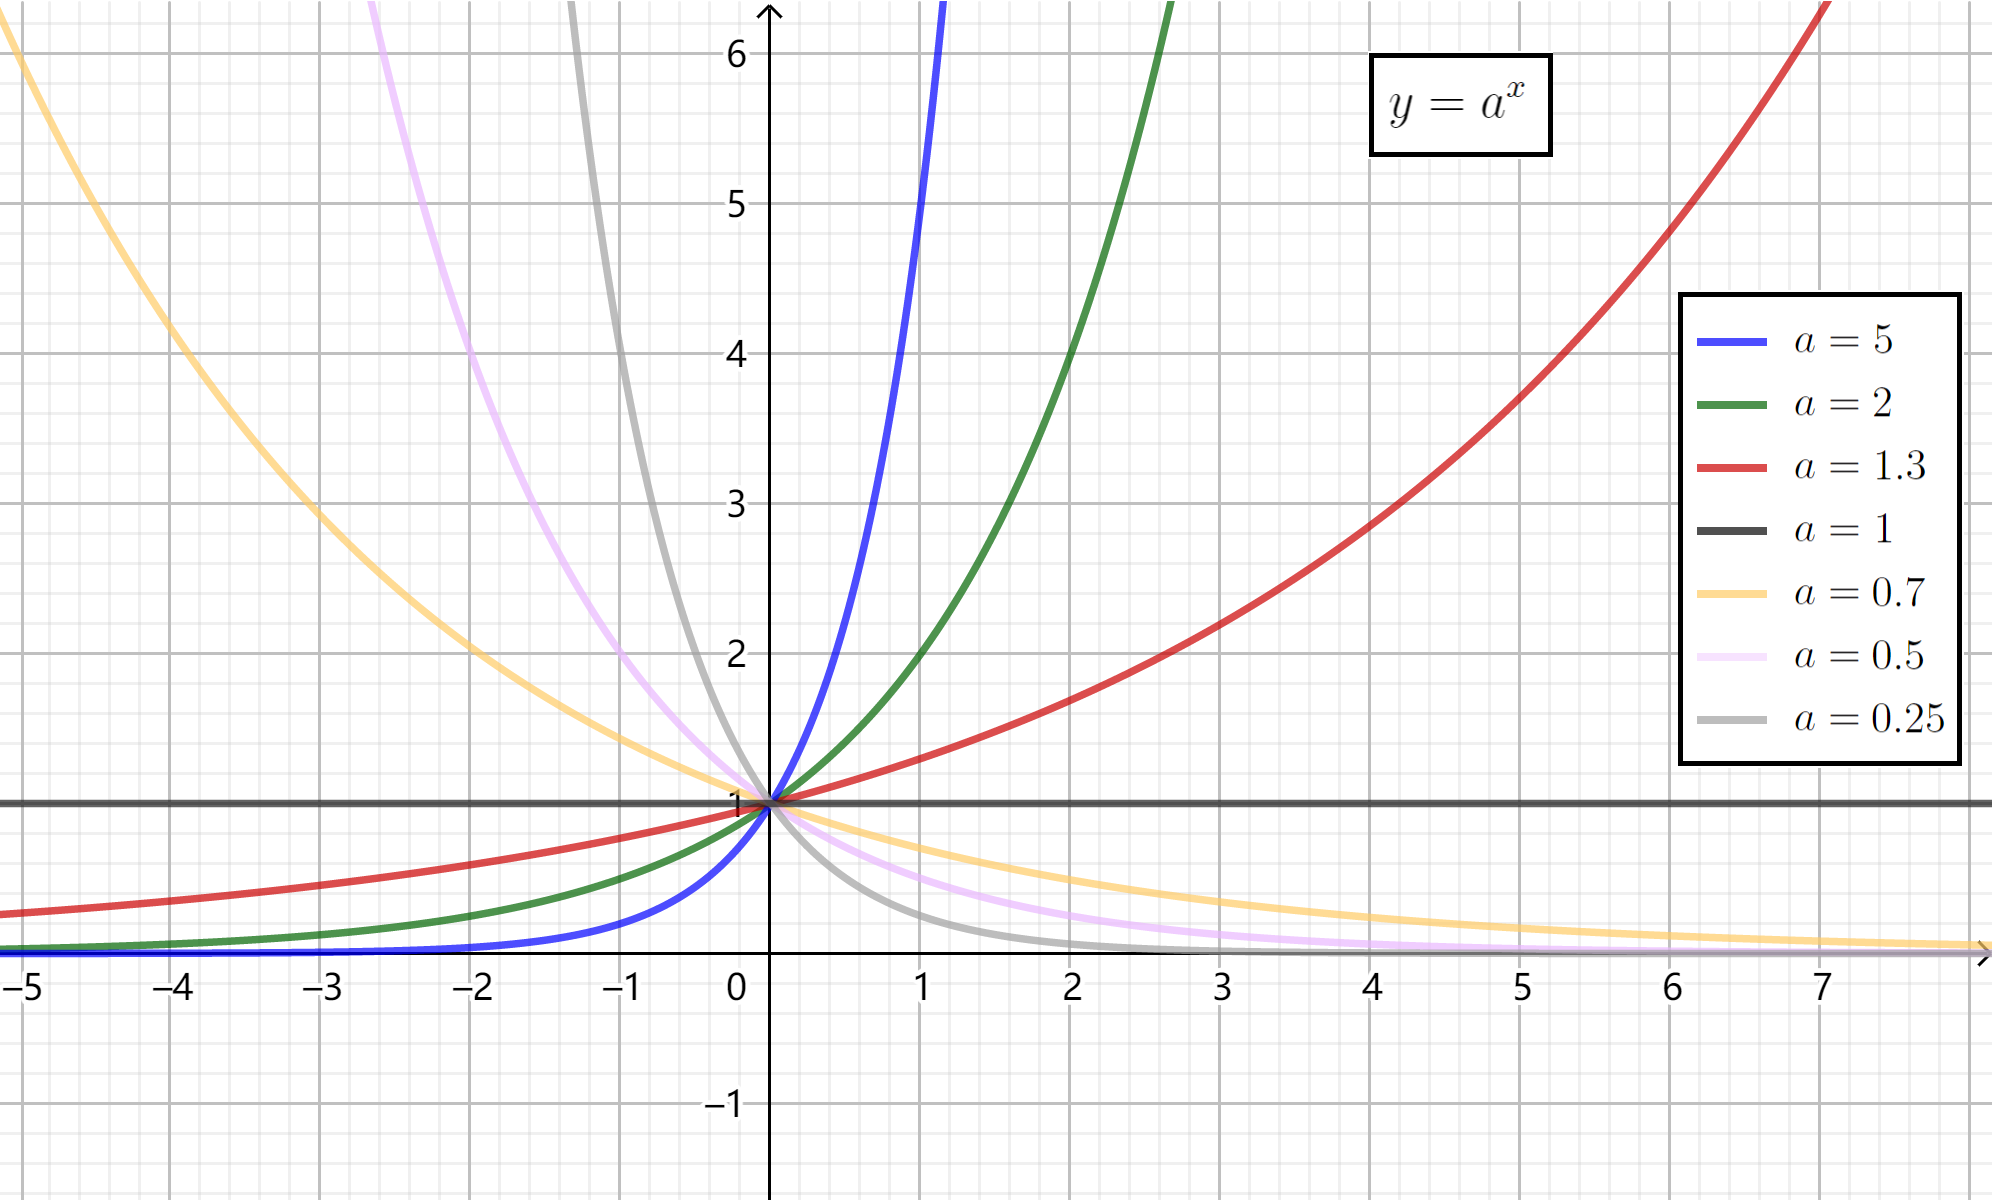
\includegraphics[width=0.96\textwidth]{指数函数1.png}
    \caption*{\texttt{指数函数}$y = a^x$\texttt{的图像}}
\end{figure}

从图像中可以发现:
\begin{enumerate}
    \item 指数函数的定义域是全体实数。
    \item 底数大于$1$时,指数函数严格单调递增。
    \begin{enumerate}[label*=\arabic*.]
        \item 自变量$x$趋于负无穷时,函数值趋于$0$。
        \item 自变量$x$趋于正无穷时,函数值趋于正无穷。
        \item $x < 0$时,函数值小于$1$,$x = 0$时,函数值等于$1$,$x > 0$时,函数值大于$1$。
        \item 函数的值域是全体正实数。
    \end{enumerate}
    \item 底数小于$1$时,指数函数严格单调递减。    
    \begin{enumerate}[label*=\arabic*.]
        \item 自变量$x$趋于负无穷时,函数值趋于正无穷。
        \item 自变量$x$趋于正无穷时,函数值趋于$0$。
        \item $x < 0$时,函数值大于$1$,$x = 0$时,函数值等于$1$,$x > 0$时,函数值小于$1$。
        \item 函数的值域是全体正实数。
    \end{enumerate}
    \item 底数等于$1$时,指数函数是常数函数$x \mapsto 1$,值域是$\{1\}$。
\end{enumerate}

底数不等于$1$时,指数函数总是单调的。所以,我们还可以定义指数函数的反函数。
我们把底数为$a$的指数函数的反函数称为底数为$a$的\textbf{对数函数},记为$\log_a$。
$$ \log_a : \,\, x \mapsto \log_a(x). $$
如果要讨论某个对任何(有效)底数都成立的性质,我们也可以忽略下标$a$,将对数函数记为$\log$。

指数函数的值域是$\mathbb{R}^+$,所以对数函数的定义域是$\mathbb{R}^+$。给定正数$u$,$\log_a(u)$就是使得$a^v = u$的唯一实数$v$。

$$ a^v = u \mbox{当且仅当} v = \log_a(u). $$

底数$a$大于$1$时,指数函数$x\mapsto a^x$严格单调递增。因此,它的反函数$\log_a$也严格单调递增。

底数$a$小于$1$时,指数函数$x\mapsto a^x$严格单调递减。因此,它的反函数$\log_a$也严格单调递减。

通过对指数函数图像作关于$y = x$的轴对称变换,我们可以画出不同底数的对数函数的图像:

\begin{figure}[h]
    \vspace{4pt}
    \centering
    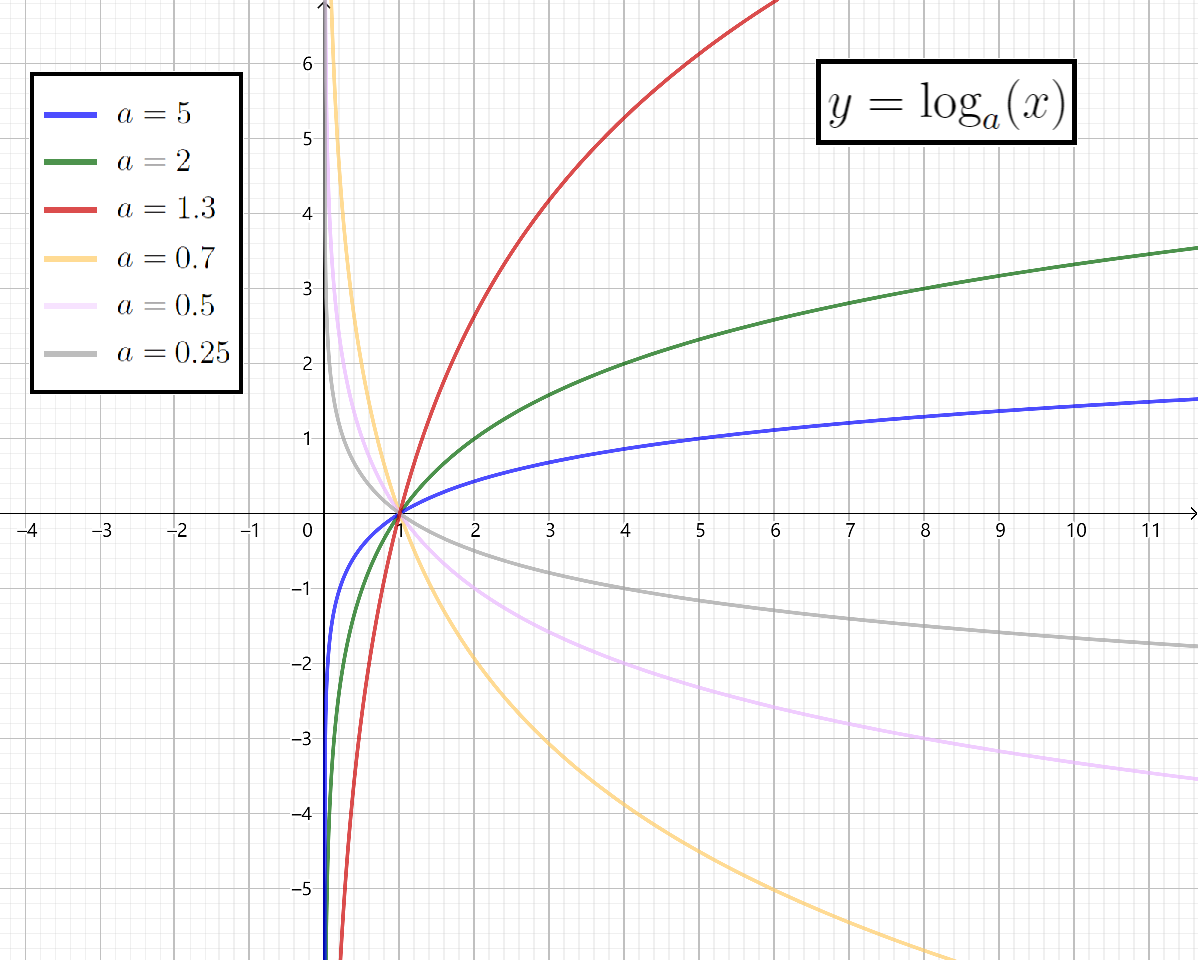
\includegraphics[width=0.96\textwidth]{对数函数1.png}
    \caption*{\texttt{对数函数}$y = \log_a(x)$\texttt{的图像}}
\end{figure}

从图像中可以发现:
\begin{enumerate}
    \item 对数函数的定义域是全体正实数,值域是$\mathbb{R}$。
    \item 底数大于$1$时,对数函数严格单调递增。
    \begin{enumerate}[label*=\arabic*.]
        \item 自变量$x$趋于$0$时,函数值趋于负无穷。
        \item 自变量$x$趋于正无穷时,函数值趋于正无穷。
        \item $x < 1$时,函数值小于$0$,$x = 1$时,函数值等于$0$,$x > 1$时,函数值大于$0$。
    \end{enumerate}
    \item 底数小于$1$时,对数函数严格单调递减。    
    \begin{enumerate}[label*=\arabic*.]
        \item 自变量$x$趋于$0$时,函数值趋于正无穷。
        \item 自变量$x$趋于正无穷时,函数值趋于负无穷。
        \item $x < 1$时,函数值大于$0$,$x = 1$时,函数值等于$0$,$x > 1$时,函数值小于$0$。
    \end{enumerate}
\end{enumerate}

注意:对数函数的底数不能是$1$。

作为指数函数的反函数,对数函数满足以下性质:
$$ \forall a, b\in\mathbb{R}^+, \log(a\cdot b) = \log(a) + \log(b). $$

指数函数和对数函数来自天文学的需求。天文学家处理各种天体之间的距离时,需要记录数值差别非常大的数据。这些数值的精确程度不高,但它们之间的比例关系比较重要。
为了方便处理这些数据,天文学家希望把乘除法运算转换为加减法运算。

为此,17世纪的数学家构造了一种对照数表。表的一侧是等差数列,另一侧是等比数列。举例来说,我们让左侧为
$0,1,2,\cdots$,右侧为$1, 10, 100, \cdots$。在左边执行加法,比如$2+3=5$,右边就执行相应的乘法:$100 \times 1000 = 100000$。
反之亦然。

天文学家的需求,是计算大数的乘除法,比如
$$329700000 \times 42100000000$$
如果我们可以找到$3\dlim{2970}\dlim{0000}$和$421\dlim{0000}\dlim{0000}$在左侧对应的数,那么将它们相加求和,再找出和左侧的位置,那么它对应的右侧的数,就是要求的乘积。

于是,不断有数学家给出详细计算的对照数表,方便相关使用者查询,简化计算。

\begin{figure}[h]
    \vspace{4pt}
    \centering
    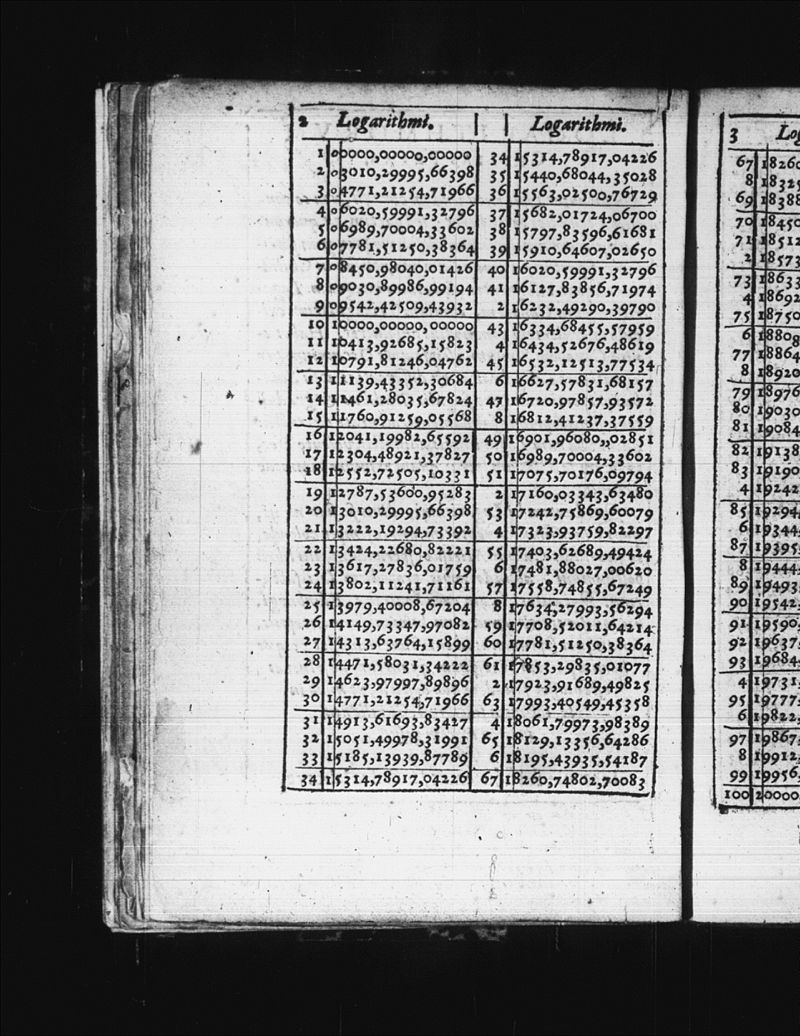
\includegraphics[width=0.6\textwidth]{Logarithmorum_Chilias_Prima_page_0-67.jpg}
    \caption*{\texttt{一份以}$10$\texttt{为底数的对照数表(17世纪)。}}
\end{figure}

从今天的角度来看,对照数表蕴含的关系就是指数和对数函数。对数就是实际计算问题中遇到的数在数表左侧对应的数,
指数就是把左侧的对数进行加减法后,指向的右侧的数,也就是计算结果。计算过程用现代的记号表示,就是:

$$ u \times v = a^{\log_a(u) + \log_a(v)}.$$

\begin{sk}
    \mbox{}\\
    \indent 1. 给定正数$a$,比较以下三个函数:$x\mapsto a^{-x}$、$x\mapsto a^{-\frac{1}{x}}$、$x\mapsto -\log_a(x)$。它们的图像有哪些相似之处?有哪些不同?
\end{sk}

\begin{xt}
    \mbox{}\\
    \indent 1. 设有定义在$\mathbb{R}$上的函数$f$,满足:$\forall \, x, y, \,\,\, f(x) \cdot f(y) = f(x + y).$\\
    \indent 1.1. 证明:$f(0)$等于$0$或$1$。以下假设$f(0) = 1.$\\
    \indent 1.2. 证明:$f(1) > 0.$\\
    \indent 1.3. 证明:对任何整数$n$,$f(n) = f(1)^n.$\\
    \indent 1.4. 证明:对任何有理数$r$,$f(r) = f(1)^r.$\\
    \indent 1.5. 如果$f$在某一点$a$处连续,证明$f$在$0$处连续。\\
    \indent 1.6. 如果$f$在某一点$a$处连续,证明$f$处处连续。\\
    \indent 1.7. 如果$f$在某一点$a$处连续,证明$f$是以$f(1)$为底的指数函数。\\
    \indent 1.8. 如果$f$是$\mathbb{R}$上的严格单调函数,用反证法证明$f$是以$f(1)$为底的指数函数。\\
    \indent 2. 设有定义在$\mathbb{R}$上的函数$g$,满足:$\forall \, x, y, \,\,\, g(x) + g(y) = g(x \cdot y).$\\
    \indent 2.1. 证明:$g(1) = 0.$\\
    \indent 2.2. 证明:对任何正数$x$以及整数$n$,$g(x^n) = n\cdot g(x).$\\
    \indent 2.3. 证明:对任何正数$x$以及有理数$r$,$g(x^r) = r\cdot g(x).$\\
    \indent 2.4. 如果$g$在某一点$a$处连续,证明$g$在$1$处连续。\\
    \indent 2.5. 如果有某个正数$c$使得$g(c) = 1$,且$g$在某一点$a$处连续,证明:对任何实数$x$,$g(c^x) = x.$\\
    \indent 2.6. 如果有某个正数$c$使得$g(c) = 1$,且$g$是$\mathbb{R}$上的严格单调函数,用反证法证明:$g$是以$c$为底的对数函数。
\end{xt}

\subsection{无穷递缩等比数列}
考虑等比数列$\{a_1 q^{n-1}\}_{n\in\mathbb{Z}^+}$,其中$q$是公比。什么情况下,$\{a_1 q^{n-1}\}_{n\in\mathbb{Z}^+}$有极限呢?我们考察它的项的绝对值:
$$|a_n| = |a_1|\cdot|q|^{n-1}$$
这个数列中所有数都大于等于$0$。其中$|a_1|$不随$n$变化。如果$a_1=0$,那么$\{a_n\}$是常数列。因此我们主要考察$a_1 \neq 0$的情况。

如果$|q|=1$,那么$|a_n| = |a_1|$,$\{|a_n|\}$是常数列。具体来说,如果$q=1$,那么$a_n = a_1$,$\{a_n\}$是常数列。
如果$q = -1$,那么$\{a_n\}$是形如$a_1, -a_1, a_1, -a_1, \cdots$的数列,相邻两项总相差$2a_1$,数列没有极限。

如果$|q| > 1$,那么随着$n$增大,$|q|^{n-1}$越来越大。$a_1 \neq 0$时,$\{|a_n|\}$是严格递增数列。只要任取正数$M$,都有正整数$N$使得
$$ |a_1||q|^{N-1} \geqslant M,$$
那么对所有比$N$大的整数$n$,$|a_n| = |a_1||q|^{n-1}$都比$M$大。于是$|a_n|$趋于正无穷大。
具体来说,如果$q$是正数,那么$a_n$在$a_1>0$时趋于正无穷大,在$a_1<0$时趋于负无穷大;如果$q$是负数,那么数列的奇数项和偶数项符号相反,
相邻两项的差是两者绝对值之和,而$|a_n|$趋于正无穷大,因此数列没有极限。

那么,任取正数$M$,是否有这样的$N$呢?我们用对数来表示$N$。如果有正整数$x$满足:
$$ |a_1||q|^{x-1} = M $$
那么$x$就可以作为我们需要的$N$。上式两边除以$|a_1|$,然后取对数,得到:
% $$ x - 1 = \log_{|q|}{\frac{M}{|a_1|}}. $$
% 解得:
$$ x = 1 + \log_{|q|}{\frac{M}{|a_1|}}. $$
但这样的$x$不一定是正整数。考虑以$|q|$为底数的指数函数,底数$|q|$比$1$大,所以它是严格递增函数。
因此,我们只需要选比$1 + \log_{|q|}{\frac{M}{|a_1|}}$大的正整数$N$,这样就有
$$ |q|^{N-1} \geqslant |q|^{x-1} = |q|^{\log_{|q|}{\frac{M}{|a_1|}}} = \frac{M}{|a_1|},$$
即
$$ |a_1||q|^{N-1} \geqslant M.$$

另一方面,如果$|q| < 1$,那么随着$n$增大,$|q|^{n-1}$越来越小。$a_1 \neq 0$时,$\{|a_n|\}$是严格递减数列。只要任取正数$r$,都有正整数$N$使得
$$ |a_1||q|^{N-1} \leqslant r,$$
那么对所有比$N$大的整数$n$,$|a_n| = |a_1||q|^{n-1}$都比$r$小。于是$|a_n|$趋于$0$。
而对数列$\{a_n\}$来说,考虑任何两个不同的正整数$n<m$,数列中对应两项的差
$$ |a_n - a_m| \leqslant |a_n| + |a_m| < 2|a_n|$$
因此,对任何正数$r$,只需令$N$为让$\forall n > N$,$|a_n| < \frac{r}{2}$的正整数,那么$\forall m, n > N$,$|a_n - a_m| < r$。
这说明数列$\{a_n\}$趋于$0$,是无穷小。

任取正数$r$,是否有这样的$N$呢?考虑以$|q|$为底数的指数函数,底数$|q|$比$1$小,所以它是严格递减函数。因此,和前一种情况类似,
我们只需要选比$x = 1 + \log_{|q|}{\frac{r}{|a_1|}}$大的正整数$N$,这样就有
$$ |q|^{N-1} \leqslant |q|^{x-1} = |q|^{\log_{|q|}{\frac{M}{|a_1|}}} = \frac{r}{|a_1|},$$
即
$$ |a_1||q|^{N-1} \leqslant r.$$

综上所述,可以将无穷等比数列$\{a_1 q^{n-1}\}_{n\in\mathbb{Z}^+}$的大体行为归纳为:

\begin{center}
    \fbox{
        \shortstack[l]{
            1. 首项为零或公比为一的等比数列是常数列。\\
            2. 公比绝对值小于一的无穷等比数列是无穷小。\\
            3. 公比大于一的无穷等比数列趋于无穷大\\
            3.1. 首项为正时,趋于正无穷大\\
            3.2. 首项为负时,趋于负无穷大\\
            4. 其他情况下,无穷等比数列不收敛。
        }
    }
\end{center}

我们通常把公比绝对值小于一的无穷等比数列称为\textbf{无穷递缩等比数列}。无穷递缩等比数列必然收敛于$0$。公比为正数时,无穷递缩等比数列是严格单调数列。
公比为负数时,无穷递缩等比数列各项的符号正负交替,绝对值不断缩小。我们也称这种数列为\textbf{交替无穷小}。

% \begin{sk}
    
% \end{sk}

\begin{xt}
    \mbox{}\\
    \indent 1. 设有首项为$a$,公比为$q$的等比数列$\{a_n\}_{n\in\mathbb{Z}^+}$。
    把$\{a_n\}$前$n$项的和记为数列$\{S_n\}_{n\in\mathbb{Z}^+}$:
    $$ \forall n \in \mathbb{Z}^+ , \quad S_n = a_1 + \cdots + a_n. $$
    如果$-1<q<1$,证明$\{S_n\}$有极限,并用$a$和$q$表示该极限。\\
    \indent 2. 数列$\{x_n\}_{n\in\mathbb{Z}^+}$满足以下关系:
    \begin{align}
        x_1 = 2, & \notag \\
        \forall n\in\mathbb{Z}^+, &\quad x_{n+1} = \frac{x_n}{3} + \frac{2}{x_n},\notag
    \end{align}
    \indent 2.1. 证明:$x_n$总在$1.5$与$2$之间.\\
    \indent 2.2. 证明:
    $$x_{n+1} - \sqrt{3} = \frac{(x_n - \sqrt{3})(x_n - 2\sqrt{3})}{3x_n}.$$
    \indent 2.3. 构造一个无穷递缩等比数列$\{a_n\}$,使得$|x_n - \sqrt{3}|$总小于$a_n$。\\
    \indent 2.4. 证明:数列$\{x_n\}_{n\in\mathbb{Z}^+}$收敛到$\sqrt{3}$。
\end{xt}

\section{极限和曲线(下)}
前面的章节中,我们讨论过极限和曲线的关系。
学习了函数的极限,了解连续函数的概念以后,我们可以用这些概念来帮助我们了解曲线。
比如,我们经常接触到的曲线,大多是连续不断的。我们可以用连续函数来严格说明,什么是连续不断的曲线。

一类基本的曲线是实变函数的图像。定义在$\mathbb{R}$上或某个区间$I$上的函数,它的图像是平面上的曲线。
如果函数是连续的,直观上,它的图像是一条连续不断的曲线。

如何说明这件事呢?我们首先需要定义,对于平面中的曲线,什么叫做连续。

\begin{df}
    给定平面$\gamma$中的曲线$c: \mathbb{R} \rightarrow \gamma$及曲线中一点$c(t_0)$,
    如果对任意正数$r$,总有$d>0$,使得只要$|t - t_0| < d$,点$c(t)$与$c(t_0)$的距离就小于$r$:
    $$ |c(t) - c(t_0)| < r,$$
    那么就说曲线$c$在$t_0$处连续或在$c(t_0)$处连续。\\
    对定义域中的区间$I$,如果对$I$中任意$t$,曲线$c$在$t$连续,就说$c$在$I$上连续。\\
    在定义域中任一点连续的曲线,称为\textbf{连续曲线}。
\end{df}

要注意的是,$c$把实数映射到平面的点,所以点$c(t)$与$c(t_0)$的距离是指两点构成的线段的长度。

对函数图像来说,函数的连续性可以推出函数图像的连续性。如果函数$f$在$t_0$处连续,那么它的图像在$t_0$处连续。
这是因为函数的图像上,$(t_0,\,\, f(t_0))$附近一点$(t,\,\, f(t))$到它的距离是:
$$ \sqrt{(t - t_0)^2 + (f(t) - f(t_0))^2} $$
根据定义,函数$f$在$t_0$处连续,那么,对任何正数$r$,都有$d>0$,使得只要$|t - t_0| < d$,
就有$|f(t) - f(t_0)| < \frac{r}{2}$。于是,取$d'$为$d$和$\frac{r}{2}$中较小者。那么$|t - t_0| < d'$时
总有:
\begin{align}
    \sqrt{(t - t_0)^2 + (f(t) - f(t_0))^2} &< \sqrt{d'^2 + \left(\frac{r}{2}\right)^2} \notag \\
    &\leqslant \sqrt{\left(\frac{r}{2}\right)^2 + \left(\frac{r}{2}\right)^2} \notag \\
    &= \frac{\sqrt{2}r}{2} < r \notag
\end{align}
这说明函数$f$的图像,作为平面中的曲线,在$t_0$连续。

实变函数的图像,作为平面中的曲线,有一个共同特征,就是与任何竖直的直线$x = x_0$至多有一个交点。
这是因为按照函数的定义,每个自变量只对应一个应变量。然而,平面中的曲线可不一定总有这样的特征。
很多曲线无法简单表示成实变函数的图像。

来看一个基本的例子:圆周。我们把圆周定义为这样的映射:$c: t\mapsto (\cos{t}, \,\, \sin{t})$。
其中$t$在区间$[0, \,\,2\pi]$中取值。

直观上,圆周也是连续不断的曲线。下面我们来严格地说明它的连续性。

给定圆周上一点$(\cos{t_0}, \,\, \sin{t_0})$。

如果$t_0 \neq 0$或$2\pi$,它附近(足够近的)一点到它的距离是:
$$ \sqrt{(\cos{t} - \cos{t_0})^2 + (\sin{t} - \sin{t_0})^2}. $$
而我们已经证明过,正弦函数和余弦函数在其定义域上是连续函数。因此,对任何正数$r$,都有$d>0$,
使得只要$|t - t_0| < d$,就有
$$ |\cos{t} - \cos{t_0}| < \frac{r}{2}, \quad |\sin{t} - \sin{t_0}| < \frac{r}{2}, $$
因此,以上的距离小于$\sqrt{\left(\frac{r}{2}\right)^2 + \left(\frac{r}{2}\right)^2} = \frac{\sqrt{2}r}{2} < r$。这说明$c$在$t_0$连续。

如果$t_0 = 0$或$2\pi$,由于$c(0) = c(2\pi)$,它附近一点$(\cos{t}, \,\, \sin{t})$要么是$t$越来越小,趋近于$0$,要么是$t$越来越大,趋近于$2\pi$。
由于正弦函数和余弦函数在$0$处连续,对于以上两种情况,我们根据:
\begin{align}
    \lian{t \to 0} \cos{t} = \cos{0}, \quad &\lian{t \to 0} \sin{t} = \sin{0}, \notag \\
    \lian{t \to 2\pi} \cos{t} = \cos{0}, \quad &\lian{t \to 2\pi} \sin{t} = \sin{0}, \notag 
\end{align}
可以得出$t$趋于$0$时,$(\cos{t}, \,\, \sin{t})$趋于$(\cos{0}, \,\, \sin{0})$;
$t$趋于$2\pi$时,$(\cos{t}, \,\, \sin{t})$也趋于$(\cos{0}, \,\, \sin{0})$。
这说明$c$在$t=0$和$t=2\pi$处,也就是$(\cos{0}, \,\, \sin{0})$处连续。

综上可知,圆周是连续曲线。

一般来说,设有曲线$c: t\mapsto (f_X(t), \,\, f_Y(t))$。如果函数$f_X, f_Y$都在某点$t_0$连续,那么$c$在$t_0$连续。
如果$f_X, f_Y$在区间$I$上连续,那么$c$在$I$上连续。如果$f_X, f_Y$在定义域上连续,那么$c$是连续曲线。

\begin{xt}
    \mbox{} \\
    \indent 1. 证明:正切函数、余切函数在其定义域上是连续函数。\\
    \indent 2. 设有曲线$c: t\mapsto (f_X(t), \,\, f_Y(t))$。证明:如果函数$f_X, f_Y$都在某点$t_0$连续,那么$c$在$t_0$连续。
\end{xt}

\chapter{不等式}

我们已经接触过一元一次、一元二次和二元一次不等式。当变量取某些值的时候,不等式成立;
取另一些值的时候,不等式不成立。这样的不等式称为\textbf{条件不等式}。如果无论变量取什么值,不等式都成立,
这样的不等式称为\textbf{绝对不等式}。

先来复习一下不等关系的定义和基本规则:
\begin{enumerate}
    \item 自反性:$\forall a, \,\,\, a \leqslant a$永远成立;
    \item 反称性:$\forall a, b, \,\,\, a \leqslant b, \,\,\, b \leqslant a$至少有一个成立;
    \item 传递性:$\forall a, b, c, \,\,\, \mbox{如果}\, a \leqslant b, \,\,\, b \leqslant c, \,\,\, \mbox{那么}\, a \leqslant c$;
    \item $\forall a, b, \,\,\, a \geqslant b$就是$b \leqslant a$;
    \item $\forall a, b, \,\,\, a < b$就是$a \leqslant b$且$a \neq b$,$ a > b$就是$a \geqslant b$且$a \neq b$。
\end{enumerate}
此外,从数的运算法则,可以得到以下定律:
\begin{enumerate}
    \item 同号的数相乘大于$0$。异号的数相乘小于$0$。
    \item (从 1 推出)任何数的平方大于等于$0$。
\end{enumerate}
这两条定律基于数的运算法则,对我们熟知的数域:$\mathbb{N}$、$\mathbb{Z}$、$\mathbb{Q}$、$\mathbb{R}$都成立。

利用这些性质,我们可以得出一些有用的结论,称为\textbf{常用不等式}。

\section{排序不等式}

给定两列数:$a_1 \geqslant a_2 \geqslant \cdots \geqslant a_n$和
$b_1 \geqslant b_2 \geqslant \cdots \geqslant b_n$。它们都按从大到小的顺序排列。
我们把数列$\{a_k\}$中最大的数乘以$\{b_k\}$中最大的数,把$\{a_k\}$中次大的数乘以$\{b_k\}$中次大的数,
以此类推,再全部加起来,把得到的和称为两列数的\textbf{顺序和}:
$$ a_1b_1 + a_2b_2 + \cdots + a_nb_n $$
我们把数列$\{a_k\}$中最大的数乘以$\{b_k\}$中最小的数,把$\{a_k\}$中次大的数乘以$\{b_k\}$中次小的数,
以此类推,再全部加起来,把得到的和称为两列数的\textbf{逆序和}:
$$ a_1b_n + a_2b_{n-1} + \cdots + a_nb_1 $$
按照其它顺序把两列数两两配对(不重复也不遗漏),加起来的和,称为两列数的\textbf{乱序和}:
$$ a_1b_{g(1)} + a_2b_{g(2)} + \cdots + a_nb_{g(n)} $$
其中$g$是某个$[1\dots n]$到自身的双射。

\begin{tm}\textbf{排序不等式}\\
    两列数的顺序和大于等于乱序和,乱序和大于等于逆序和。
\end{tm}
\begin{proof}
    我们用归纳法证明。设命题$P(n)$:若有$a_1 \geqslant a_2 \geqslant \cdots \geqslant a_n$和
    $b_1 \geqslant b_2 \geqslant \cdots \geqslant b_n$,那么
    $$ \sum_{i=1}^n a_ib_i \geqslant \sum_{i=1}^n a_ib_{g(i)} \geqslant \sum_{i=1}^n a_ib_{n+1-i} . $$
    其中$g$是$[1\dots n]$到自身的双射。

    $P(1)$显然为真。来看$P(2)$。顺序和为$a_1b_1 + a_2b_2$,乱序和与逆序和都是$a_1b_2 + a_2b_1$。两者作差:
    $$ a_1b_1 + a_2b_2 - (a_1b_2 + a_2b_1) = (a_1 - a_2)(b_1 - b_2) $$
    右侧的$a_1-a_2$和$b_1-b_2$都大于等于零,因此乘积大于等于零。
    这就证明$a_1b_1 + a_2b_2 \geqslant a_1b_2 + a_2b_1$。于是$P(2)$为真。

    假设$P(n)$为真。下面证明$P(n+1)$为真。设有两列数:
    $a_1 \geqslant a_2 \geqslant \cdots \geqslant a_n\geqslant a_{n+1}$
    和$b_1 \geqslant b_2 \geqslant \cdots \geqslant b_n \geqslant b_{n+1}$。
    设$c_1, c_2, \cdots , c_{n+1}$是打乱顺序后的数列$\{b_k\}$。
    考虑乱序和$\sum_{i=1}^{n+1} a_i c_i$。先证明乱序和小于等于顺序和。

    对$c_{1}$分情况讨论。

    如果$c_1$就是$b_1$,那么
    $$\sum_{i=1}^{n+1} a_i c_i = a_1b_1 + \sum_{i=2}^{n+1} a_i c_i.$$
    $c_2, \cdots, c_{n+1}$
    是$b_2, \cdots, b_{n+1}$打乱顺序。所以根据归纳假设$P(n)$,
    $\sum_{i=2}^{n+1} a_i c_i \leqslant \sum_{i=2}^{n+1} a_i b_i$。
    因此
    $$\sum_{i=1}^{n+1} a_i c_i \leqslant \sum_{i=1}^{n+1} a_i b_i.$$
    如果$c_1$不是$b_1$,某个$c_j$是$b_1$,我们希望把$c_1$调成$b_1$,这样就回到了上一种情况。
    只要保证这样调整之后乱序和不变小就可以了。由于$a_1 \geqslant a_j$,$c_1 \leqslant c_j = b_1$,
    根据$P(2)$,逆序和$a_1c_1 + a_jc_j$小于等于顺序和$a_1c_j + a_jc_1$。所以把$c_1$和$c_j$互换,
    得到的乱序和比原来的乱序和更大。而新的乱序和中$c_1$就是$b_1$,因此小于等于顺序和。
    这说明原来的乱序和小于等于顺序和。

    综上所述,任何情况下,乱序和小于等于顺序和。

    再来证明逆序和小于等于乱序和。
    如果$c_1$是$b_{n+1}$,那么
    $$\sum_{i=1}^{n+1} a_i c_i = a_1b_{n+1} + \sum_{i=2}^{n+1} a_i c_i.$$
    $c_2, \cdots, c_{n+1}$是$b_1, \cdots, b_{n}$打乱顺序。所以根据归纳假设$P(n)$,
    $\sum_{i=2}^{n+1} a_i c_i \geqslant \sum_{i=2}^{n+1} a_i b_{n+2-i}$。
    因此
    $$\sum_{i=1}^{n+1} a_i c_i \geqslant \sum_{i=1}^{n+1} a_i b_{n+2-i}.$$
    如果$c_1$不是$b_{n+1}$,某个$c_j$是$b_{n+1}$,我们希望把$c_1$调成$b_{n+1}$,这样就回到了上一种情况。
    只要保证这样调整之后乱序和不变大就可以了。由于$a_1 \geqslant a_j$,$c_1 \geqslant c_j = b_{n+1}$,
    根据$P(2)$,顺序和$a_1c_1 + a_jc_j$大于等于逆序和$a_1c_j + a_jc_1$。所以把$c_1$和$c_j$互换,
    得到的乱序和比原来的乱序和更小。而新的乱序和中$c_1$就是$b_{n+1}$,因此大于等于逆序和。
    这说明原来的乱序和大于等于逆序和。

    综上所述,任何情况下,乱序和大于等于逆序和。
    
    因此,对任何正整数$n$,$P(n)$为真。
\end{proof}

\begin{xt}    
    \mbox{}\\
    \indent 1. 给定两列数:$a_1 \geqslant a_2 \geqslant \cdots \geqslant a_n$和
$b_1 \geqslant b_2 \geqslant \cdots \geqslant b_n$。\\
    \indent 1.1 试把$(a_1 + a_2 + \cdots + a_n)(b_1 + b_2 + \cdots + b_n)$用这两列数的顺序和、乱序和与逆序和表示。\\
    \indent 1.2 证明:$(a_1 + a_2 + \cdots + a_n)(b_1 + b_2 + \cdots + b_n)$小于等于顺序和的$n$倍,大于等于逆序和的$n$倍。 \\
    \indent 2. 给定正数$a,b,c$。证明:$(a + b + c)(\frac{1}{a}+\frac{1}{b}+\frac{1}{c}) \geqslant 9$。
\end{xt}

\section{内积不等式}

我们已经看过平面向量的内积不等式:
$$
(a_1^2 + a_2^2)(b_1^2 + b_2^2) = (a_1b_1 + a_2b_2)^2 + (a_1b_2 - a_2b_1)^2 \geqslant (a_1b_1 + a_2b_2)^2
$$
向量模长平方之积等于内积和面积的平方和,因此大于内积的平方。这个不等式也可以写成:
$$
\sqrt{(a_1^2 + a_2^2)(b_1^2 + b_2^2)} \geqslant |a_1b_1 + a_2b_2|
$$
对于多元有序数组$(a_1, a_2, \cdots, a_n)$和$(b_1, b_2, \cdots, b_n)$,
\begin{align}
&(a_1^2 + a_2^2 + \cdots + a_n^2)(b_1^2 + b_2^2 + \cdots + b_n^2) \notag \\
=\,\,& (a_1b_1 + a_2b_2 + \cdots + a_nb_n)^2 + \frac{1}{2}\sum_{i=1}^n\sum_{j=1}^n(a_ib_j - a_jb_i)^2 \notag \\
\geqslant\,\,& (a_1b_1 + a_2b_2 + \cdots + a_nb_n)^2 \notag 
\end{align}
其中$\frac{1}{2}\sum_{i=1}^n\sum_{j=1}^n(a_ib_j - a_jb_i)^2$的“来历”为:
\begin{align}
&\left(\sum_{i=1}^n a_i^2\right) \left(\sum_{j=1}^n b_j^2\right) - \left(\sum_{i=1}^n a_ib_i\right)^2 \notag \\
=\,\,& \sum_{i=1}^n\sum_{j=1}^n a_i^2 \cdot b_j^2 - \sum_{i=1}^n\sum_{j=1}^n a_ib_i\cdot a_jb_j \notag \\
=\,\,& \frac{1}{2}\left(\sum_{i=1}^n\sum_{j=1}^n (a_ib_j)^2 + \sum_{i=1}^n\sum_{j=1}^n (a_jb_i)^2 -  2 \sum_{i=1}^n\sum_{j=1}^n a_ia_jb_ib_j \right) \notag \\
=\,\,& \frac{1}{2}\sum_{i=1}^n\sum_{j=1}^n \left( (a_ib_j)^2 + (a_jb_i)^2 -  2 a_ib_j\cdot a_jb_i \right) \notag \\ 
=\,\,& \frac{1}{2}\sum_{i=1}^n\sum_{j=1}^n \left( a_ib_j - a_jb_i \right)^2. \notag 
\end{align}

因此,对一般的$n$,也有内积不等式:
$$ \sqrt{(a_1^2 + a_2^2 + \cdots + a_n^2)(b_1^2 + b_2^2 + \cdots + b_n^2)} \geqslant |a_1b_1 + a_2b_2+ \cdots + a_nb_n|$$

\begin{xt}    
    \mbox{}\\
    \indent 1. 给定正数$a,b,c$。证明:$(a + b + c)(\frac{1}{a}+\frac{1}{b}+\frac{1}{c}) \geqslant 9$。\\
    \indent 2. 给定正数$a,b,c$。证明:$(ab^2 + bc^2 + ca^2)(ab + bc + ca) \geqslant abc(a+b+c)^2$ \\
    \indent 3. 给定正数$a$,求$2a + \frac{1}{a^2}$的最小值。
\end{xt}

\section{诸均值不等式}

平均值是一种描述数据的方法。我们已经学习过算术平均值。给定$n$个正数:$a_1, a_2, \cdots , a_n$,
它们的算术平均值是:
$$ m_A : \,\,\, a_1, a_2, \cdots , a_n \mapsto \frac{a_1 + a_2 + \cdots + a_n}{n}. $$
除了算术平均值,生产实践中还会用到其它几种平均值。几何平均值来自射影定理,用乘积开方得到结果:
$$ m_G :\,\,\, a_1, a_2, \cdots , a_n \mapsto  (a_1a_2\cdots a_n)^{\frac{1}{n}}.$$
调和平均值来自音乐中对和弦的研究,它是倒数的算术平均值的倒数:
$$ m_H : \,\,\, a_1, a_2, \cdots , a_n \mapsto \left(\frac{a_1^{-1} + a_2^{-1} + \cdots + a_n^{-1}}{n}\right)^{-1}. $$
这三种平均值都源自古典数学,是研究平面与空间形体、音律、天文地理时常见的工具。它们之间有什么联系呢?

首先来看两个数的情况。给定两个正数$a_1$、$a_2$,它们的算术平均值是$\frac{a_1 + a_2}{2}$,几何平均值是$\sqrt{a_1a_2}$,调和平均值是$\frac{2a_1a_2}{a_1 + a_2}$。我们发现:
\begin{align}
    \frac{a_1 + a_2}{2} - \sqrt{a_1a_2} &= \frac{1}{2}(\sqrt{a_1} - \sqrt{a_2})^2 \geqslant 0 \notag \\
    \sqrt{a_1a_2} - \frac{2a_1a_2}{a_1 + a_2} &= \frac{2\sqrt{a_1a_2}}{a_1 + a_2}\left(\frac{a_1 + a_2}{2} - \sqrt{a_1a_2}\right) \geqslant 0 \notag
\end{align}
任意两正数$a_1$、$a_2$的算术平均值总大于等于几何平均值,几何平均值总大于等于调和平均值。

再来看三个数的情况给定两个正数$a_1$、$a_2$、$a_3$,它们的算术平均值是$\frac{a_1 + a_2 + a_3}{3}$,几何平均值是$\sqrt[3]{a_1a_2a_3}$,调和平均值是$\frac{3a_1 a_2 a_3}{a_1 a_2 + a_2 a_3 + a_3 a_1}$。
\begin{align}
    &\frac{a_1 + a_2 + a_3}{3} - \sqrt[3]{a_1a_2a_3} \notag \\
    =\,\,& \frac{1}{6}(\sqrt[3]{a_1} + \sqrt[3]{a_2} + \sqrt[3]{a_3})\left((\sqrt[3]{a_1} - \sqrt[3]{a_2})^2 + (\sqrt[3]{a_2} - \sqrt[3]{a_3})^2 + (\sqrt[3]{a_3} - \sqrt[3]{a_1})^2\right) \notag \\
    \geqslant\,\,&0. \notag \\
    &\sqrt[3]{a_1a_2a_3} - \frac{3a_1 a_2 a_3}{a_1 a_2 + a_2 a_3 + a_3 a_1} \notag \\
    =\,\,& \frac{3\sqrt[3]{a_1a_2a_3}}{a_1 a_2 + a_2 a_3 + a_3 a_1}\left(\frac{a_1 a_2 + a_2 a_3 + a_3 a_1}{3} - \sqrt[3]{a_1^2a_2^2a_3^2}\right) \notag \\
    =\,\,& \frac{3\sqrt[3]{a_1a_2a_3}}{a_1 a_2 + a_2 a_3 + a_3 a_1}\left(\frac{a_1 a_2 + a_2 a_3 + a_3 a_1}{3} - \sqrt[3]{(a_1a_2)(a_2a_3)(a_3a_1)}\right) \notag \\
    \geqslant \,\,&0. \notag
\end{align}

于是,任意三正数$a_1$、$a_2$、$a_3$的算术平均值总大于等于几何平均值,几何平均值总大于等于调和平均值。

这让我们猜想,是否任何$n$个正数$a_1, a_2, \cdots , a_n$,它们的算术平均值总大于等于几何平均值,几何平均值总大于等于调和平均值?

先证明算术平均值总大于等于几何平均值。设命题$P(n)$:
$n$个正数的算术平均值总大于等于几何平均值。对于$n=2,3$的情况,我们使用了因式分解来证明。
这种方法难以推广。使用$P(2)$,我们可以证明以下较“弱”的结论:如果$P(n)$成立,那么$P(2n)$成立。
\begin{align}
    \frac{a_1 + a_2 + \cdots a_{2n}}{2n} &\geqslant \frac{1}{2}\left((a_1a_2\cdots a_{n})^{\frac{1}{n}} + (a_{n+1}a_{n+2}\cdots a_{2n})^{\frac{1}{n}} \right) \notag \\
    &\geqslant \sqrt{(a_1a_2\cdots a_{n})^{\frac{1}{n}} \cdot (a_{n+1}a_{n+2}\cdots a_{2n})^{\frac{1}{n}}} \notag \\
    &= (a_1a_2\cdots a_{2n})^{\frac{1}{2n}}\notag
\end{align}

因此,通过归纳法我们可以证明,只要$n$是$2$的乘方,那么$P(n)$为真。对于剩余的$n$,我们要另想办法。
由于已经证明了$P(n)$对足够大的$n$为真,我们可以把归纳法“反过来用”:假设$P(n)$对某个$n$为真,
可以证明$P(n-1)$为真。

若$P(n)$为真,给定正数$a_1, a_2, \cdots , a_{n-1}$,我们补上第$n$个数$a_n$,以便使用归纳假设。
令$a_n$为$n-1$个数的算术平均值:$a_n = \frac{a_1 + a_2 + \cdots + a_{n-1}}{n-1}$。
这样,将$a_n$补到前$n-1$个数里,不改变算术平均值。
$$ \frac{a_1 + a_2 + \cdots + a_n}{n} = \frac{a_1 + a_2 + \cdots + a_{n-1}}{n-1} = a_n. $$
$P(n)$为真,所以
$$ a_n = \frac{a_1 + a_2 + \cdots + a_n}{n} \geqslant (a_1a_2\cdots a_{n})^{\frac{1}{n}}. $$
两边取$n$次方,消去右侧$a_n$,得到$a_n^{n-1} \geqslant a_1a_2\cdots a_{n-1}$。因此
$$   \frac{a_1 + a_2 + \cdots + a_{n-1}}{n-1} = a_n \geqslant (a_1a_2\cdots a_{n-1})^{\frac{1}{n-1}}. $$
于是$P(n-1)$也为真。

整理一下以上的讨论。我们首先证明了,只要$n$是$2$的乘方,那么$P(n)$为真。
接下来我们证明了,若$P(n)$为真,$P(n-1)$也为真。给定任何正整数$n>1$,如果$n$是$2$的乘方,那么$P(n)$为真。
如果$n$不是$2$的乘方,那么总可以找到$2$的乘方$2^m$大于$n$。$P(2^m)$为真,因此$P(2^m-1)$为真,
因而$P(2^m-2)$为真……依此类推,$2^m-n$步之后,就得到$P(n)$为真。因此,无论$n$是不是$2$的乘方,$P(n)$都为真。

以上证明可算是归纳法的一种“升级改良”。我们无法直接用$P(n)$到$P(n+1)$来归纳出所有$P(n)$为真,
于是先通过归纳法解决一部分$n$,再通过反向“补漏”的方法,解决剩余的$n$。

证明了算术平均值总大于等于几何平均值,再证明几何平均值总大于等于调和平均值。

给定$n$个正数$a_1, a_2, \cdots , a_n$,记它们的几何平均值为$G$,另外构造$n$个正数:
$\frac{G}{a_1}, \frac{G}{a_2}, \cdots , \frac{G}{a_n}$。它们的算术平均值大于等于几何平均值:
$$ \frac{G}{a_1} + \frac{G}{a_2} + \cdots + \frac{G}{a_n} \geqslant n\left(\frac{G}{a_1}\frac{G}{a_2}\cdots \frac{G}{a_n}\right)^{\frac{1}{n}} = \frac{nG^\frac{n}{n}}{(a_1a_2\cdots a_{n})^{\frac{1}{n}}} = n.$$
因此
$$ G \geqslant n \left(a_1^{-1} + a_2^{-1} + \cdots + a_n^{-1}\right)^{-1} =  \left(\frac{a_1^{-1} + a_2^{-1} + \cdots + a_n^{-1}}{n}\right)^{-1}. $$
除了算术平均值、几何平均值和调和平均值,生产实践中还会用到不少别的平均值。不少平均值之间也存在类似的绝对不等关系。

% \begin{align}
%     \left(1 + \frac{1}{n}\right)^{n+2} &= (n+2)^{n+2} \cdot \left(\frac{(n+1)\cdot \frac{1}{n+1} + \frac{1}{n}}{n+2}\right)^{n+2} \notag \\
%     &\geqslant (n+2)^{n+2} \cdot \frac{1}{(n+1)^{n+1}} \cdot \frac{1}{n} \notag \\
%     &= 
% \end{align}

\begin{xt}    
    \mbox{}\\
    \indent 1. 给定正数$a,b,c$。证明:$(a + b + c)(\frac{1}{a}+\frac{1}{b}+\frac{1}{c}) \geqslant 9$。\\
    \indent 2. 给定正数$a,b,c$。证明:$(ab^2 + bc^2 + ca^2)(ab + bc + ca) \geqslant abc(a+b+c)^2$。 \\
    \indent 3. 设数列$\{e_n\}$的通项公式为:
    $$ \forall n\in\mathbb{Z}^+,\quad e_n = \left(1 + \frac{1}{n}\right)^n.$$
    \indent 3.1. 证明:$\{e_n\}$是严格单调递增数列\footnote{提示:把$1 + \frac{1}{n+1}$表示成$n+1$个数的和。}。\\
    \indent 3.2. 设数列$\{w_n\}$的通项公式为:
    $$ \forall n\in\mathbb{Z}^+,\quad w_n = \left(1 + \frac{1}{n}\right)^{n+1}.$$
    证明它是严格单调递减数列\footnote{提示:把$1 + \frac{1}{n}$表示成$n+2$个数的和。}。 \\
    \indent 3.3. 证明:$\{e_n\}$有极限,记为$e$。\\
    \indent 3.4. 证明:$2 < e < 3$。
\end{xt}


\begin{appendix}

\chapter{从数列到实数}
\section{数列极限的基本性质}

\begin{tm}\label{tm:a-0-10}
    数列$\{a_n\}$收敛到$x$,则它的任何子列也收敛到$x$。
\end{tm}
\begin{proof}
    记子列为$\{b_n\}$,$\{b_n\}$的元素$b_1,b_2,b_3,\cdots$在原数列的下标为:$1\leqslant k_1<k_2<k_3<\cdots$。
    这说明$k_n \geqslant n$。数列$\{a_n\}$收敛到$x$,按照定义,对任何$r>0$,总有正整数$N$,使得对所有$n>N$,都有
    $ |a_n - x| < r$。对所有$n>N$,$k_n>n>N$,所以$|b_n - x| = |a_{k_n} - x| < r$。这说明子列$\{b_n\}$收敛到$x$。
\end{proof}

\begin{tm}\label{tm:a-0-20}
    已知数列$\{a_n\}$收敛,它的某个子列$\{b_n\}$收敛到$x$,则$\{a_n\}$也收敛到$x$。
 \end{tm}
\begin{proof}
    子列$\{b_n\}$收敛到$x$。记$\{b_n\}$的元素$b_1,b_2,b_3,\cdots$在原数列的下标为:
    $1\leqslant k_1<k_2<k_3<\cdots$。则$k_n \geqslant n$。设$\{a_n\}$的极限为$y$。
    按照定义,对任何$r>0$,由于$\frac{r}{2} > 0$,总有正整数$N_a$,使得对所有$n>N_a$,都有$ |a_n - y| < \frac{r}{2}$。
    同理也有正整数$N_b$,使得对所有$n>N_b$,都有$ |b_n - x| < \frac{r}{2}$。
    于是,只要取$N$为$N_a$、$N_b$中较大的,那么对所有$n>N$,都有$|b_n - x| < \frac{r}{2}$且$ |a_{k_n} - y| < \frac{r}{2}$。
    因此,
    $$|x - y| \leqslant |x - a_{k_n}| + |a_{k_n} - y| = |b_n - x| + |a_{k_n} - y| < \frac{r}{2} + \frac{r}{2} = r. $$
    这说明$y = x$,即$\{a_n\}$也收敛到$x$。
\end{proof}

\begin{tm}{\textbf{收敛数列有界}}\label{tm:a-0-30}
    有极限的数列必然是有界数列。
\end{tm}
\begin{proof}
    设数列$\{a_n\}$收敛到$x$。按照定义,对$1$来说,有正整数$N$,使得只要$n>N$,就有$|a_n - x| < 1$。这说明$n>N$时,
    总有$x - 1 < a_n < x + 1$。设$U$是数列前$N$项中最大的,$V$是前$N$项中最小的。那么数列的任一项总小于$U+1$和$x+1$中较大者,
    总大于$V-1$和$x-1$中较小者。这就说明$\{a_n\}$有界。
\end{proof}

\begin{tm}{\textbf{数列极限的不等关系传递}}\label{tm:a-0-40}
    设数列的元素在数集$T$中。已知数列$\{a_n\}$收敛到$T$中元素$x$。
    \begin{enumerate}
        \item 如果$\{a_n\}$的项总小于等于某个数$u$,则$x$小于等于$u$。
        \item 如果$\{a_n\}$的项总小于某个数$u$,则$x$小于等于$u$。
        \item 如果$\{a_n\}$的项总大于等于某个数$u$,则$x$大于等于$u$。
        \item 如果$\{a_n\}$的项总大于某个数$u$,则$x$大于等于$u$。
    \end{enumerate}
\end{tm}
\begin{proof}
    我们使用反证法证明这几个命题。\\
    证明(1)、(2):反设$x > u$。由于$d = x - u > 0$,存在正整数$N$,使得只要$n>N$,就有$|a_n - x| < d$。这说明
    $a_n > x - d = u$,矛盾!\\
    证明(3)、(4):反设$x < u$。由于$d = u - x > 0$,存在正整数$N$,使得只要$n>N$,就有$|a_n - x| < d$。这说明
    $a_n < x + d = u$,矛盾!
\end{proof}

\textbf{注意}:数列的项总小于(大于)某个数$u$,不表示$x$一定严格小于(大于)$u$。$x$是有可能等于$u$的。举例来说,数列$\{\frac{1}{n}\}_{n\in\mathbb{Z}^+}$
每项都大于$0$,但它的极限等于$0$。我们说“\textbf{极限传递不等号时,别忘了加等号}”。

不仅数列与数之间的不等关系可以通过极限传递,数列与数列之间的不等关系也可以传递。

\begin{df}
    给定两数列$\{a_n\}$、$\{b_n\}$,如果两者对应的项总存在同一种不等关系,就说两数列之间存在该不等关系。
\end{df}
举例来说,如果对任意正整数$n$,总有$a_n \leqslant b_n$,就说$\{a_n\}$小于等于$\{b_n\}$。
在不至于混淆的时候,我们可以简单将其记为$\{a_n\} \leqslant \{b_n\}$。

\begin{tm}{\textbf{数列极限传递不等关系}}\label{tm:a-0-45}
    设数列的元素在数集$T$中。已知数列$\{a_n\}$、$\{b_n\}$分别收敛到$T$中元素$x,y$。
    \begin{enumerate}
        \item 如果$\{a_n\} \leqslant \{b_n\}$,则$x\leqslant y$。
        \item 如果$\{a_n\} < \{b_n\}$,则$x\leqslant y$。
        \item 如果$\{a_n\} \geqslant \{b_n\}$,则$x\geqslant y$。
        \item 如果$\{a_n\} > \{b_n\}$,则$x\geqslant y$。
    \end{enumerate}
\end{tm}
\begin{proof}
    我们使用反证法证明这几个命题。\\
    证明(1)、(2):反设$x > y$。由于$d = \frac{x - y}{2} > 0$,存在正整数$N_a$,使得只要$n>N_a$,就有$|a_n - x| < d$。
    同理,存在正整数$N_b$,使得只要$n>N_b$,就有$|b_n - y| < d$。这说明,$n$大于$N_a,N_b$中较大者的时候,
    $a_n > x - d = y + d > b_n$,矛盾!\\
    证明(3)、(4):反设$x < y$。由于$d = \frac{x - y}{2} > 0$,存在正整数$N_a$,使得只要$n>N_a$,就有$|a_n - x| < d$。
    同理,存在正整数$N_b$,使得只要$n>N_b$,就有$|b_n - y| < d$。这说明,$n$大于$N_a,N_b$中较大者的时候,
    $a_n < x - d = y + d < b_n$,矛盾!\\
\end{proof}

\textbf{注意}:同样,两数列的项满足严格小于(大于)关系,不表示极限$x$一定严格小于(大于)$y$。$x$是有可能等于$y$的。举例来说,数列$\{\frac{1}{n}\}_{n\in\mathbb{Z}^+}$
每项都大于$\{-\frac{1}{n}\}_{n\in\mathbb{Z}^+}$对应的项,但它的极限都等于$0$。再次强调:\textbf{极限传递不等号时,别忘了加等号}。

数列之间的不等关系可以通过极限传递,但极限只描述数列的大体行为,不描述数列具体的项的性质。我们可以设想这样的情景:
一个数列每一项都比另一个数列大,但这两个数列收敛到同一个极限。这种情况下,如果有第三格数列每项都在两者之间,那么由于“上下”都趋于同一个数,
第三个数列夹在其中,也只能趋于这个数了。这个结论称为\textbf{同归定理}。
\begin{tm}{\textbf{同归定理}}\label{tm:a-0-48}
    如果数列$\{a_n\}$小于(等于)$\{b_n\}$,$\{b_n\}$小于(等于)$\{c_n\}$,而$\{a_n\}$、$\{c_n\}$有同样的极限$x$,那么$\{b_n\}$也收敛到$x$。
\end{tm}
\begin{proof}
    按照定义,对任意正数$r>0$,存在正整数$N_a$,使得只要$n>N_a$,就有$|a_n - x| < r$。
    同理,存在正整数$N_c$,使得只要$n>N_c$,就有$|c_n - y| < r$。这说明,$n$大于$N_a,N_c$中较大者的时候,
    总有
    $$ x - r < a_n \leqslant b_n \leqslant c_n < x + r. $$
    因此$\{b_n\}$也收敛到$x$。
\end{proof}

同归定理是非常有用的结论,在证明、寻找数列极限时经常用到。

\begin{tm}{\textbf{无穷小的运算律}}\label{tm:a-0-50}
    无穷小是收敛到$0$的数列。设有元素在数集$T$中的数列$\{a_n\}$和$\{b_n\}$,$\{a_n\}$是无穷小。
    \begin{enumerate}
        \item $\{|a_n|\}$也是无穷小。
        \item 如果$\{b_n\}$也是无穷小,那么$\{a_n + b_n\}$、$\{a_n - b_n\}$、$\{a_n\cdot b_n\}$是无穷小。
        \item 如果存在$T$中正数$M$以及正整数$N$,使得$n>N$时总有$|b_n| \leqslant M\cdot |a_n|$,那么$\{b_n\}$也是无穷小。
    \end{enumerate}
\end{tm}
\begin{proof}
    \mbox{} \\
    (1). $\{a_n\}$是无穷小。按照定义,对任何$T$中正数$r$,存在正整数$N$,使得$n>N$时总有$|a_n - 0| < r$。这说明$\big||a_n| - 0\big| = \big||a_n|\big| = |a_n| < r$。
    因此$\{|a_n|\}$也是无穷小。\\
    (2). 如果$\{b_n\}$也是无穷小,按照极限的运算律,$\{a_n \pm b_n\}$趋于$0 \pm 0 = 0$,$\{a_n \cdot b_n\}$趋于$0 \cdot 0 = 0$,因此都是无穷小。\\
    (3). $\{a_n\}$是无穷小。按照定义,对任何$T$中正数$r$,由于$\frac{r}{M} > 0$,存在正整数$N$,使得$n>N$时总有$|a_n - 0| < \frac{r}{M}$。因此,$n>N$时总有
    \begin{align}
        |b_n - 0| &\leqslant M\cdot |a_n| \notag \\ 
        &< M\cdot \frac{r}{M} = r.  \notag
    \end{align}
    因此$\{b_n\}$也是无穷小。
\end{proof}

\begin{tm}\label{tm:a-0-60}
    自敛数列总是有界数列。
\end{tm}
\begin{proof}
    设数列$\{a_n\}$是自敛数列。按照定义,对$1$来说,有正整数$N$,使得只要$n,m>N$,就有$|a_n - a_m| < 1$。这说明$n>N$时,
    总有$a_{N+1} - 1 < a_n < a_{N+1} + 1$。设$U$是数列前$N$项中最大的,$V$是前$N$项中最小的。那么数列的任一项总小于$U+1$和$a_{N+1}+1$中较大者,
    总大于$V-1$和$a_{N+1}-1$中较小者。这就说明$\{a_n\}$有界。
\end{proof}

\begin{tm}\label{tm:a-0-70}
    有极限的数列是自敛数列。
\end{tm}
\begin{proof}
    设有数列$\{a_n\}$,其元素是数集$T$的元素,并收敛到$T$中某个元素$x$。对$T$中任意正数$r>0$,由于$\frac{r}{2}>0$,
    按照定义,总有正整数$N$,使得只要$n>N$,就有$|a_n - x| < \frac{r}{2}$。于是,对任意$m,n>N$,
    $$ |a_n - a_m| = |a_n - x - (a_m - x)| \leqslant |a_n - x| + |a_m - x| < \frac{r}{2} + \frac{r}{2} = r.$$
    这说明$\{a_n\}$是自敛数列。
\end{proof}

推论:有极限的数列总是有界数列。

\begin{tm}{\textbf{收敛数列控制自敛数列}}\label{tm:a-0-80}
    已知有元素在数集$T$中的数列$\{a_n\}$、$\{b_n\}$。其中$\{b_n\}$趋于$0$,
    如果对任意正整数$n$,都有正整数$N$,使得只要$m,k>N$,就有$|a_k - a_m| < b_n$,那么$\{a_n\}$是自敛数列。
\end{tm}
\begin{proof}
    对任意$T$中正数$r$,首先可以找到正整数$N_b$,使得$n>N_b$时总有$|b_n| < r$。于是,按照条件,存在正整数$N$,使得只要$m,k>N$,就有
    $$|a_k - a_m| < b_n \leqslant |b_n| < r.$$
    这说明$\{a_n\}$是自敛数列。
\end{proof}

\section{实数的构造}

\begin{tm}\label{tm:a-1-3}
    自敛有理数列经过四则运算仍然是自敛有理数列\footnote{除法中作为被除数的数列的绝对值数列有大于$0$的下界。}。
\end{tm}
\begin{proof}
    \mbox{} \\
    \textbf{加减法}:设有元素在数集$T$中的自敛数列$\{a_n\}, \{b_n\}$。对$T$中任意正数$r$,记$r_1=\frac{r}{2}$,则$r_1>0$,按照定义,有正整数$N_a, N_b$,
    使得只要$n,m>N_a$,就有$|a_n - a_m| < r_1$;只要$n,m>N_b$,就有$|b_n - b_m| < r_1$。
    因此,只要取$N$为$N_a, N_b$中较大者,那么$n,m>N$时,总有$|a_n - a_m| < r_1$、$|b_n - b_m| < r_1$同时成立。于是
    $$ |a_n \pm b_n - (a_m \pm b_m)| = |a_n - a_m \pm (b_n - b_m)| \leqslant |a_n - a_m| + |b_n - b_m| < r_1 + r_1 = r. $$
    因此数列$\{a_n \pm b_n\}$也是自敛数列。\\
    \textbf{乘法}:设有元素在数集$T$中的自敛数列$\{a_n\}, \{b_n\}$。定理\ref{tm:a-1-10}说明它们都是有界数列。因此有$T$中元素$M_a, M_b>0$,使得
    $|a_n|$总小于$M_a$、$|b_n|$总小于$M_b$。取$M$为$M_a, M_b$中较大者,那么,$|a_n|$、$|b_n|$都总小于$M$。\\    
    对$T$中任意正数$r$,记$r_1 = \frac{r}{2M}$,则$r_1>0$。因此,按照定义,有正整数$N_a, N_b$,使得只要$n,m>N_a$,
    就有$|a_n - a_m| < r_1$;只要$n,m>N_b$,就有$|b_n - b_m| < r_1$。
    因此,只要取$N$为$N_a, N_b$中较大者,那么$n,m>N$时,总有$|a_n - a_m| < r_1$、$|b_n - b_m| < r_1$同时成立。
    于是:
    \begin{align}
        |a_nb_n - a_mb_m| &= |(a_n - a_m)b_n + a_m(b_n - b_m)| \notag \\
        &\leqslant |(a_n - a_m)b_n| + |a_m(b_n - b_m)| = |a_n - a_m|\cdot |b_n| + |b_n - b_m|\cdot|a_m| \notag \\
        &< \frac{r}{2M} \cdot M + \frac{r}{2M} \cdot M = r \notag
    \end{align}
    因此数列$\{a_n b_n\}$也是自敛数列。\\
    \textbf{除法}:设有元素在数集$T$中的自敛数列$\{a_n\}, \{b_n\}$。其中$b_n$的绝对值总大于$T$中元素$d$($d > 0$)。
    定理\ref{tm:a-0-60}说明$\{a_n\}$是有界数列,也就是说,有$T$中元素$M$,使得$|a_n|$总小于$M$。
    对$T$中任意正数$r$,记$r_1 = \frac{d^2}{M+d}r$,则$r_1>0$。按照定义,有正整数$N_a, N_b$,使得只要$n,m>N_a$,
    就有$|a_n - a_m| < r_1$;只要$n,m>N_b$,就有$|b_n - b_m| < r_1$。
    因此,只要取$N$为$N_a, N_b$中较大者,那么$n,m>N$时,总有$|a_n - a_m| < r_1$、$|b_n - b_m| < r_1$同时成立。
    于是:
    \begin{align}
        \left|\frac{a_n}{b_n} - \frac{a_m}{b_m}\right| &= \frac{|a_nb_m - a_mb_n|}{|b_nb_m|} \notag \\
        &= \frac{|(a_n - a_m)b_m - a_m(b_n - b_m)|}{|b_n||b_m|} \notag \\
        &\leqslant \frac{|a_n - a_m||b_m|}{|b_n||b_m|} + \frac{|a_m||b_n - b_m|}{|b_n||b_m|}\notag \\
        &= \frac{|a_n - a_m|}{|b_n|} + \frac{|a_m||b_n - b_m|}{|b_n||b_m|} \notag \\
        &< \frac{r_1}{d} + \frac{Mr_1}{d^2} \notag \\
        &= \frac{M+d}{d^2} r_1 = r \notag
    \end{align} 
    因此数列$\{\frac{a_n}{b_n}\}$也是自敛数列。\\
\end{proof}

\begin{tm}\label{tm:a-1-5}
    有理数是实数。
\end{tm}
\begin{proof}
    任何有理数$q$,考虑常数列$\{q\}$。它是自敛有理数列,因此收敛到一个实数。而$\{q\}$显然收敛到$q$,因此$q$是实数。
\end{proof}

\begin{df}\textbf{实数的相等关系}
    设实数$a$、$b$分别是自敛有理数列$\{a_n\}, \{b_n\}$的极限,定义两者之间的二元关系如下:
    $a = b$当且仅当$\{a_n - b_n\}$趋于$0$。称之为相等关系。
\end{df}

\begin{tm}\label{tm:a-1-10}
    实数的相等关系是等价关系。
\end{tm}
\begin{proof}
    \mbox{} \\
    \textbf{自反性}:对任意实数$a$,设$a$为自敛有理数列$\{a_n\}$的极限。$\{a_n - a_n\}$是零数列,因此趋于$0$。这说明$a = a$。\\
    \textbf{对称性}:对任意实数$a, b$,设$a$为自敛有理数列$\{a_n\}$的极限,$b$为自敛有理数列$\{b_n\}$的极限。
    记$u_n = a_n - b_n$。那么,$a = b$也就是说$\{u_n\}$趋于$0$。因此$\{b_n - a_n\} = \{-u_n\}$也趋于$0$,因此$b = a$。\\
    \textbf{传递性}:对任意实数$a, b$,设它们分别是自敛有理数列$\{a_n\}, \{b_n\}, \{c_n\}$的极限。如果$a=b$、$b=c$,
    就是说数列$\{a_n - b_n\}$、$\{b_n - c_n\}$趋于$0$,因此它们的和数列趋于$0+0=0$。而它们的和数列是$\{a_n - c_n\}$。这说明$a=c$。
\end{proof}

考虑所有自敛有理数列的集合$\mathcal{R}$,所有极限相等的自敛有理数列都构成$\mathcal{R}$的一个子集。
每个自敛有理数列恰属于一个子集。这些子集构成了$\mathcal{R}$的分划。

我们说每个子集是一个等价类。每个实数恰好对应一个等价类,每个等价类也恰好对应一个实数。因此,我们可以用这些等价类来表示实数。
实数$a$对应的等价类里,每个趋于$a$的自敛有理数列,都是$a$的一种表现形式。
就好比$\frac{2}{4}$和$\frac{3}{6}$是同一个有理数的不同表现形式一样。

等价类的一个基本性质:
\begin{tm}\label{lm:a-1-10}
    两个等价类要么交集为空,要么相等。    
\end{tm}
\begin{proof}
    设$A,B$是集合$X$中按照等价关系$\leftrightarrows$定义的等价类。如果$A,B$交集不为空集,即有$x\in X$,$x\in A$且$x\in B$。\\
    对任意$a\in A$,$a\leftrightarrows x\in B$,说明$a\in B$;\\
    对任意$b\in B$,$b\leftrightarrows x\in A$,说明$b\in A$。于是$A\subseteq B$、$B\subseteq A$,即$A = B$。\\
\end{proof}

这个结论说明,如果某等价类有一个元素在另一个等价类中,那么两个等价类是同一个等价类。

\begin{tm}\label{tm:a-1-15}
    实数的不等关系满足:
    \begin{enumerate}
        \item \textbf{自背性}:$\forall a$,$a < a$不成立。
        \item \textbf{三分律}:$\forall a, b$,$a < b$,$a > b$,$a = b$恰有一个成立。
        \item \textbf{传递性}:$\forall a, b, c$,如果$a < b$、$b < c$,则$a < c$。如果$a > b$、$b > c$,则$a > c$。
    \end{enumerate}
\end{tm}
\begin{proof}
    \mbox{} \\
    \textbf{自背性}: $\forall a$,设$\{a_n\}$是收敛到$a$的自敛有理数列,则$\{a_n - a_n\}$是零数列,
    不存在正整数$N$使得$\{a_n - a_n\}$自第$N$项后总大于零。因此$a<a$不成立。\\
    \textbf{三分律}: $\forall a, b$,如果$a = b$,那么两者对应同一个等价类,从上一条性质可知,$a<b$、$b<a$都不成立。\\
    如果$a = b$不成立,那么存在分别收敛到$a,b$的自敛数列$\{a_n\}, \{b_n\}$,其差数列$\{a_n - b_n\}$仍然是自敛有理数列,但极限不是$0$。
    也就是说,存在某个有理数$r>0$,使得对任何正整数$m$,都有$n>m$,$|a_n - b_n - 0| > r$。\\
    另一方面,由于$\{a_n - b_n\}$自敛,所以对于$\frac{r}{2}$,存在正整数$N$,使得只要$n,m>N$,$|a_n - b_n - (a_m - b_m)| < \frac{r}{2}$。
    这说明,只要$m>N$,那么先找到使得$|a_n - b_n - 0| > r$的$n$,然后就可以得到:
    \begin{align}
        |a_m - b_m| \geqslant |a_n - b_n| - |a_n - b_n - (a_m - b_m)| > r - \frac{r}{2} = \frac{r}{2} \notag 
    \end{align}
    这说明,只要$m>N$,要么$a_m - b_m > \frac{r}{2}$,要么$a_m - b_m < -\frac{r}{2}$。\\
    然而,如果对某两个正整数$k>m>N$,
    有$a_k - b_k > \frac{r}{2}$且$a_m - b_m < -\frac{r}{2}$,那么$|a_k - b_k - (a_m - b_m)| > \frac{r}{2} - (-\frac{r}{2}) = r > \frac{r}{2}$。
    这与前面$\{a_n - b_n\}$自敛得到的结论矛盾!所以,两种情况不可能同时存在。
    要么对任意$m>N$,都有$a_m - b_m > \frac{r}{2}$;要么对任意$m>N$,都有$a_m - b_m < -\frac{r}{2}$。\\
    不妨设前一种情况成立。这时我们找到了分别收敛到$a,b$的自敛数列$\{a_n\}, \{b_n\}$,以及正整数$N$,
    使得对任意$n>N$,都有$a_n - b_n > \frac{r}{2}$。考虑其他收敛到$a,b$的自敛有理数列$\{a_n'\}, \{b_n'\}$,
    按照定义有$\{a_n - a_n'\}$和$\{b_n - b_n'\}$趋于$0$。因此,对$\frac{r}{8}>0$,有正整数$N_a,N_b$,
    使得只要$n>N_a$,就有$|a_n - a_n' - 0| < \frac{r}{8}$,只要$n>N_b$,就有$|b_n - b_n' - 0| < \frac{r}{8}$。
    于是,只要取正整数$N'$为$N,N_a,N_b$中的最大者,就有
    \begin{align}
        a_n' - b_n' &= a_n - b_n - (a_n - a_n') - (b_n - b_n') \notag \\
        &> \frac{r}{2} - \frac{r}{8} - \frac{r}{8} \notag \\
        &= \frac{r}{4} > 0. \notag
    \end{align}
    这个结论对任何收敛到$a,b$的自敛有理数列$\{a_n'\}, \{b_n'\}$都成立,所以$a>b$。\\
    类似地,如果设后一种情况成立,我们找到了分别收敛到$a,b$的自敛数列$\{a_n\}, \{b_n\}$,以及正整数$N$,
    使得对任意$n>N$,都有$a_n - b_n < -\frac{r}{2}$。按照同样的方法,我们可以证明对任何收敛到$a,b$的自敛有理数列$\{a_n'\}, \{b_n'\}$,
    都有正整数$N'$,使得$\{a_n' - b_n'\}$自第$N'$项往后都小于零,所以$a<b$。\\
    综上,我们证明了$\forall a, b$,$a < b$,$a > b$,$a = b$恰有一个成立。\\
    \textbf{传递性}:$\forall a, b, c$,如果$a < b$、$b < c$,那么对任何分别收敛到$a,b,c$的自敛有理数列$\{a_n\}$、$\{b_n\}$、$\{c_n\}$,
    总有正整数$N_{(a,b)}$和$N_{(b,c)}$,使得自敛数列$\{a_n - b_n\}$、$\{b_n - c_n\}$分别自第$N_{(a,b)}$项和$N_{(b,c)}$项往后总大于零。
    因此,只要取正整数$N$为$N_{(a,b)}$和$N_{(b,c)}$中较大者,那么对任意$n>N$,
    $$ a_n - c_n = a_n - b_n + b_n - c_n < 0.$$
    这说明$a<c$。\\
    同理可以证明,$\forall a, b, c$,如果$a > b$、$b > c$,则$a > c$。
\end{proof}

\textbf{注意}:我们没有直接证明\textbf{反对称性}:“$a<b$当且仅当$b>a$”。这个结论很有用,可以从以上三个性质推出。

\begin{tm}\label{tm:a-1-18}
    非零实数与$0$之间总有有理数。
\end{tm}
\begin{proof}
    设有实数$a\neq 0$。考虑收敛到$a$的自敛有理数列$\{a_n\}$。它的极限不是$0$,
    说明存在某个有理数$r>0$,使得对任何正整数$n$,都有$m>n$,$|a_m - 0| > r$。
    另一方面,数列$\{a_n\}$自敛,所以对于$\frac{r}{2} > 0$,存在正整数$N$,使得只要$n,m>N$,$|a_m - a_n| < \frac{r}{2}$。
    于是,只要$n>N$,我们先找到$m>n$,使得$|a_m| > r$,那么:
    $$  |a_n| \geqslant |a_m| - |a_m - a_n| > r - \frac{r}{2} = \frac{r}{2}. $$
    也就是说,只要$n>N$,要么$a_n > \frac{r}{2}$,要么$a_n < -\frac{r}{2}$。
    从数轴上看,自第$N$项往后,数列$\{a_n\}$的项要么在$\frac{r}{2}$右边,要么在$-\frac{r}{2}$左边。下面我们用反证法证明,不可能有“分处两边”的情况。
    反设有某两个数$n,m>N$,使得$a_m > \frac{r}{2}$,而$a_n < -\frac{r}{2}$,那么
    $$a_m - a_n > \frac{r}{2} - (-\frac{r}{2}) = r.$$
    但我们已经知道,$\forall \,\,n,m>N$,$|a_m - a_n| < \frac{r}{2}$。矛盾!\\
    所以要么$\forall\,\, n>N$,$a_n > \frac{r}{2}$,要么$\forall\,\, n>N$,$a_n < -\frac{r}{2}$。\\
    前一种情况下,考虑任一收敛到$a$的数列$\{a_n'\}$,按照定义,$\{a_n - a_n'\}$趋于$0$。因此,对$ \frac{r}{4} > 0$,有正整数$N'$,
    使得只要$n>N'$,就有$|a_n - a_n'| < \frac{r}{4}$。于是,只要$n$大于$N,N'$中较大者,就有
    $$ a_n' > a_n - (a_n - a_n') > \frac{r}{2} - \frac{r}{4} = \frac{r}{4}.$$
    这说明$a > \frac{r}{4} > 0$。\\
    后一种情况下,用类似的方式可以证明$a < -\frac{r}{4} < 0$。\\
    综上所述,非零实数$a$与$0$之间总有有理数。
\end{proof}

\begin{tm}\label{tm:a-1-20}
    实数可以定义四则运算。实数的四则运算与有理数一致,并且满足加法、乘法的结合律与交换律,以及乘法对加法的分配律。
\end{tm}
\begin{proof}
    给定实数$a$、$b$,设它们分别对应自敛有理数列的等价类$A,B$。
    按照定义,两数的和、差、积、商($b\neq 0$)分别是:
    \begin{itemize}
        \item $a \pm b = \{\{a_n \pm b_n\} \, |\, \{a_n\}\in A,\,\,\{b_n\}\in B \}$
        \item $a\cdot b = \{\{a_n \cdot b_n\} \, |\, \{a_n\}\in A,\,\,\{b_n\}\in B \}$
        \item $a\div b = \left.\left\{\left\{\frac{a_n}{b_n}\right\} \, \right|\, \{a_n\}\in A,\,\,\{b_n\}\in B \right\}$
    \end{itemize}
    首先证明这些定义自洽,即$a\pm b$、$a\cdot b$、$a\div b$是自敛有理数列的等价类,因而对应某个实数。\\
    对任意$\{a_n\}\in A,\,\,\{b_n\}\in B$,根据定理\ref{tm:a-1-3},数列$\{a_n\}, \{b_n\}$的和、差、积、商($b\neq 0$)都是自敛有理数列。
    如果对另外任意的$\{a_n'\}\in A,\,\,\{b_n'\}\in B$,可以证明$\{a_n'\}, \{b_n'\}$的和、差、积、商与$\{a_n\}, \{b_n\}$的和、差、积、商的差都是无穷小:
    \begin{align}
        \{a_n \pm b_n - (a_n' \pm b_n')\} &\to 0 \notag \\
        \{a_nb_n - a_n'b_n'\} &\to 0 \notag \\
        \{\frac{a_n}{b_n} - \frac{a_n'}{b_n'}\} &\to 0 \notag 
    \end{align}
    那么$a\pm b$、$a\cdot b$、$a\div b$都是等价类。于是$a\pm b$、$a\cdot b$、$a\div b$是自敛有理数列的等价类。这样就完成了证明。\\
    下面给出证明:\\
    按照等价类的定义,$\{a_n - a_n'\}$和$\{b_n - b_n'\}$都趋于$0$。\\
    \textbf{和差}:注意到$a_n \pm b_n - (a_n' \pm b_n') = (a_n - a_n') \pm (b_n - b_n')$,因此趋于$0$。\\
    \textbf{积}:计算$a_nb_n - a_n'b_n'$。根据定理\ref{tm:a-0-60},$\{a_n\}, \{b_n\}$都是有界数列。即存在$M>0$,使得$|a_n|$、$|b_n|$总小于$M$。
    \begin{align}
        |a_nb_n - a_n'b_n'| &= |a_n(b_n - b_n') + (a_n - a_n')b_n'| \notag \\
        &\leqslant |a_n||b_n - b_n'| + |a_n - a_n'||b_n'| \notag \\
        &\leqslant M(|b_n - b_n'| + |a_n - a_n'|) \notag 
    \end{align}
    对任何有理数$r>0$,$r_1 = \frac{r}{2M}>0$,因此,总有正整数$N_a,N_b$,
    使得只要$n>N_a$,就有$|a_n - a_n' - 0| < r_1$,只要$n>N_b$,就有$|b_n - b_n' - 0| < r_1$。
    于是,只要取正整数$N$为$N_a,N_b$中较大者,就有
    $$ |a_nb_n - a_n'b_n'| < M\cdot \left(r_1 + r_1\right) = r.$$
    这说明数列$\{a_nb_n - a_n'b_n'\}$趋于$0$。\\
    \textbf{商}:$b\neq 0$,因此要么$b>0$,要么$b<0$。不妨设$b>0$。计算$\frac{a_n}{b_n} - \frac{a_n'}{b_n'}$。
    根据定理\ref{tm:a-0-60},$\{a_n\}, \{b_n\}$都是有界数列。即存在$M>0$,使得$|a_n|$、$|b_n|$总小于$M$。
    另一方面,由于$b>0$,根据定理\ref{tm:a-1-18},可以取有理数$d$使得$b>d>0$。因此,存在正整数$N$使得只要$n>N$,就有$b_n>d$、$b_n'>d$。
    \begin{align}
        \left|\frac{a_n}{b_n} - \frac{a_n'}{b_n'}\right| &= \frac{|a_nb_n' - a_n'b_n|}{|b_n||b_n'|} \notag \\
        &= \frac{|a_n(b_n' - b_n) + (a_n - a_n')b_n|}{|b_n||b_n'|} \notag \\
        &\leqslant \frac{|a_n||b_n - b_n'|}{|b_n||b_n'|} + \frac{|a_n - a_n'||b_n|}{|b_n||b_n'|} \notag \\
        &= \frac{|a_n||b_n - b_n'|}{|b_n||b_n'|} + \frac{|a_n - a_n'|}{|b_n'|} \notag \\
        &< \frac{M}{d^2}|b_n - b_n'| + \frac{1}{d}|a_n - a_n'|) \notag 
    \end{align}
    对任何有理数$r>0$,$r_1 = \frac{rd^2}{M+d}>0$,因此,总有正整数$N_a,N_b$,
    使得只要$n>N_a$,就有$|a_n - a_n'| < r_1$,只要$n>N_b$,就有$|b_n - b_n' - 0| < r_1$。
    于是,只要取正整数$N$为$N_a,N_b$中较大者,就有
    $$ \left|\frac{a_n}{b_n} - \frac{a_n'}{b_n'}\right| < r_1\cdot \left(\frac{M}{d^2} + \frac{1}{d}\right) = \frac{rd^2}{M+d}\cdot \frac{M+d}{d^2} = r.$$
    这说明数列$\{\frac{a_n}{b_n} - \frac{a_n'}{b_n'}\}$趋于$0$。\\
    证明了实数的四则运算自洽,接下来证明\textbf{实数的四则运算满足运算律}。\\
    \textbf{加法交换律}:考察集合$a + b = \{\{a_n + b_n\} \, |\, \{a_n\}\in A,\,\,\{b_n\}\in B \}$、
    $b + a = \{\{b_n + a_n\} \, |\, \{a_n\}\in A,\,\,\{b_n\}\in B \}$可知两者相同。这说明$a + b = b + a$。\\
    \textbf{乘法交换律}:考察集合$a\cdot b = \{\{a_n \cdot b_n\} \, |\, \{a_n\}\in A,\,\,\{b_n\}\in B \}$、
    $b\cdot a = \{\{b_n \cdot a_n\} \, |\, \{a_n\}\in A,\,\,\{b_n\}\in B \}$可知两者相同。这说明$a \cdot b = b \cdot a$。\\
    \textbf{加法结合律}:给定实数$a$、$b$、$c$,设它们分别对应自敛有理数列的等价类$A,B,C$。考察
    \begin{align}
        (a + b) + c &= \{\{(a_n + b_n) + c_n\} \, |\, \{a_n\}\in A,\,\,\{b_n\}\in B,\,\,\{c_n\}\in C \} \notag \\
        a + (b + c) &= \{\{a_n + (b_n + c_n)\} \, |\, \{a_n\}\in A,\,\,\{b_n\}\in B,\,\,\{c_n\}\in C \} \notag
    \end{align}
    可知两集合相同。$(a + b) + c = a + (b + c)$。\\
    \textbf{乘法结合律}:考察
    \begin{align}
        (a \cdot b) \cdot c &= \{\{(a_n \cdot b_n) \cdot c_n\} \, |\, \{a_n\}\in A,\,\,\{b_n\}\in B,\,\,\{c_n\}\in C \} \notag \\
        a \cdot (b \cdot c) &= \{\{a_n \cdot (b_n \cdot c_n)\} \, |\, \{a_n\}\in A,\,\,\{b_n\}\in B,\,\,\{c_n\}\in C \} \notag
    \end{align}
    可知两集合相同。$(a \cdot b) \cdot c = a \cdot (b \cdot c)$。\\
    \textbf{乘法对加法的分配律}:考察
    \begin{align}
        (a + b) \cdot c &= \{\{(a_n + b_n) \cdot c_n\} \, |\, \{a_n\}\in A,\,\,\{b_n\}\in B,\,\,\{c_n\}\in C \} \notag \\
        a \cdot c + b \cdot c &= \{\{a_n \cdot c_n + b_n \cdot c_n\} \, |\, \{a_n\}\in A,\,\,\{b_n\}\in B,\,\,\{c_n\}\in C \} \notag
    \end{align}
    可知两集合相同。$(a + b) \cdot c = a \cdot c + b \cdot c$。类似可以证明$a \cdot (b + c) = a \cdot b + a \cdot c$。\\
    最后证明\textbf{实数的四则运算与有理数一致}。按照定理\ref{tm:a-1-5},有理数都是实数。因此只要验证以下的基本性质:
    \begin{enumerate}
        \item 任何实数与零的和是自己。
        \item 任何实数与零的积是零。
        \item 任何实数与一的积是自己。
        \item 实数减法是加法的逆运算:$\forall \,\, a, b, \,\,\, a - b + b = a + b - b = a.$
        \item 实数减法是加法的逆运算:$\forall \,\, a, b(\neq 0), \,\,\, a \div b \times b = a\times b \div b = a.$
    \end{enumerate}
    (1). 给定实数$a$,记$a$对应的等价类为$A$。考虑$a+0$对应的等价类:$A_0 = \{ \{a_n + b_n\} \,|\, \{a_n\}\to a, \,\, \{b_n\} \to 0 \}$。
    按照定义,$A_0$的元素总与$A$的某个元素相差一个无穷小,因此也是$A$的元素。
    % 反之,$A$中元素总可以写成自身与零数列的和,而零数列趋于$0$,因此$A$中元素总是$A_0$的元素。
    这说明$A = A_0$,即$a + 0 = a$。同理可证$0+a=a$。\\
    (2). 给定实数$a$,记$a$对应的等价类为$A$。考虑$a\cdot 0$对应的等价类:$A_0 = \{ \{a_n \cdot b_n\} \,|\, \{a_n\}\to a, \,\, \{b_n\} \to 0 \}$。
    根据定理\ref{tm:a-0-30},$\{a_n\}$是有界数列,因此根据定理\ref{tm:a-0-50},$\{a_nb_n\}$趋于$0$。$A_0$的元素总是无穷小,因此是$0$的等价类。即$a \cdot 0 = a$。同理可证$0\cdot a=a$。\\
    (3). 考虑$a\cdot 1$对应的等价类:$A_0 = \{\{a_n \cdot b_n\} \,|\, \{a_n\}\to a, \,\, \{b_n\} \to 1 \}$。
    考虑$A_0$的元素$\{a_n \cdot b_n\}$,其中$\{a_n\}\to a$,$\{b_n\} \to 1$。由于$a_n \cdot b_n - a_n = a_n \cdot (b_n - 1)$,
    所以按照极限的乘法,$\{a_n \cdot b_n - a_n\}$趋于$a(1 - 1) = 0$。这说明$\{a_n \cdot b_n\}$是$A$的元素。
    % 反之,$A$中元素$\{a_n\}$总可以写成$\{a_n\cdot 1\}$,因此是$A_0$的元素。
    这说明$A = A_0$,即$a \cdot 1 = a$。同理可证$1 \cdot a = a$。\\
    (4). 考虑$a - b + b$等价类中的元素,它能写成形如$\{a_n - b_n + b_n'\}$的数列,其中$\{a_n\}$收敛到$a$,$\{b_n\}$、$\{b_n\}$收敛到$b$。
    因此$\{b_n - b_n'\}$收敛到$0$,$\{a_n - b_n + b_n'\}$与$\{a_n\}$相差一个无穷小,因此收敛到$a$。
    % 反之,收敛到$a$的数列$\{a_n\}$总能写成$\{a_n - b_n + b_n\}$的形式,其中$\{b_n\}$是任意收敛到$b$的数列。
    这说明$a - b + b = a$。同理可证$a + b - b = a.$\\
    (5). 考虑$a \div b \times b$等价类中的元素,他能写成形如$\{a_n \div b_n \times b_n'\}$的数列,其中$\{a_n\}$收敛到$a$,$\{b_n\}$、$\{b_n\}$收敛到$b$。
    考虑数列$\{\frac{a_n b_n}{b_n'} - a_n\}$。
    $\{a_n\}$收敛到$a$,所以是有界数列,可以找到有理数$M$使得$|a_n|$总小于$M$。$b\neq 0$,所以可以找到$0$与$b$之间的有理数$d$,以及正整数$N$,使得只要$n>N$,就有$|b_n| > d$。
    于是$n>N$时总有:
    \begin{align}
        \left|\frac{a_n b_n}{b_n'} - a_n\right| &= \frac{\left|a_n\right| \left|b_n - b_n'\right|)}{\left|b_n'\right|} \notag \\
        &< \frac{M}{d}\left|b_n - b_n'\right| \notag
    \end{align}
    而$\{b_n - b_n'\}$收敛到$0$,所以根据定理\ref{tm:a-0-50},数列$\{\frac{a_n b_n}{b_n'} - a_n\}$收敛到$0$。
    % 反之,收敛到$a$的数列$\{a_n\}$总能写成$\{\frac{a_n b_n}{b_n}\}$的形式,其中$\{b_n\}$是任意收敛到$b$的数列。
    这说明$a \div b \times b = a$。同理可证$a\times b \div b = a.$\\
\end{proof}

\begin{tm}\label{tm:a-1-25}
    实数的相等关系与四则运算兼容:
    \begin{enumerate}
        \item 等式两边加上(减去)同一个实数,仍然相等。
        \item 等式两边乘以同一个实数,仍然相等。
        \item 等式两边除以同一个非零实数,仍然相等。
    \end{enumerate}
\end{tm}
\begin{proof}
    设等式两边的值是实数$a=b$。\\
    (1). 在等式两边加上(减去)实数$c$,
    左边得到$a\pm c$,右边得到$b\pm c$。对$a\pm c$、$b\pm c$中任意元素,它们分别能写成$\{a_n\pm c_n\}$、$\{b_n\pm c_n'\}$的形式。其中$\{a_n\}$、$\{b_n\}$
    收敛到$a$、$b$,$\{c_n\}$、$\{c_n'\}$收敛到$c$。$\{a_n\pm c_n-(b_n\pm c_n')\} = \{a_n - b_n \pm  (c_n - c_n')\}$趋于$0$。这说明
    $a\pm c = b\pm c$。\\
    (2). 在等式两边乘以实数$c$,左边得到$a\cdot c$,右边得到$b\cdot c$。对$a\cdot c$、$b\cdot c$中任意元素,
    它们分别能写成$\{a_n\cdot c_n\}$、$\{b_n\cdot c_n'\}$的形式。其中$\{a_n\}$、$\{b_n\}$
    收敛到$a$、$b$,$\{c_n\}$、$\{c_n'\}$收敛到$c$。注意到
    \begin{align}
        a_n\cdot c_n - b_n\cdot c_n' &= (a_n - b_n)\cdot c_n + b_n\cdot(c_n - c_n') \notag \\
    \end{align}
    通过极限的运算可知$\{a_n\cdot c_n - b_n\cdot c_n'\}$收敛到$(a - b)c + b(c - c) = 0$。这说明$a\cdot c = b\cdot c$。\\
    (3). 在等式两边除以非零实数$c$,左边得到$a\div c$,右边得到$b\div c$。对$a\div c$、$b\div c$中任意元素,
    它们分别能写成$\{\frac{a_n}{c_n}\}$、$\{\frac{b_n}{c_n'}\}$的形式。其中$\{a_n\}$、$\{b_n\}$
    收敛到$a$、$b$,$\{c_n\}$、$\{c_n'\}$收敛到$c$。注意到
    \begin{align}
        \frac{a_n}{c_n} - \frac{b_n}{c_n'} &= \frac{a_nc_n' - b_nc_n}{c_nc_n'} \notag \\
        &= \frac{(a_n - b_n)\cdot c_n' - b_n\cdot(c_n - c_n')}{c_nc_n'}
    \end{align}
    通过极限的运算可知$\{\frac{a_n}{c_n} - \frac{b_n}{c_n'}\}$收敛到$\frac{(a - b)c + b(c - c)}{c^2} = 0$。这说明$a\div c = b\div c$。\\
\end{proof}

\begin{tm}\label{tm:a-1-30}
    实数的不等关系与四则运算兼容:
    \begin{enumerate}
        \item 不等式两边加上(减去)同一个实数,关系不变。
        \item 同号不等式相加,关系不变。
        \item 不等式两边乘以同一个正实数,关系不变;乘以同一个负实数,关系反号。
    \end{enumerate}
\end{tm}
\begin{proof}
    设不等关系为小于关系,不等式两边的值分别是实数$a<b$。\\
    (1). 在不等式两边加上(减去)实数$c$,
    左边得到$a\pm c$,右边得到$b\pm c$。对$a\pm c$、$b\pm c$中任意元素,它们分别能写成$\{a_n\pm c_n\}$、$\{b_n\pm c_n'\}$的形式。其中$\{a_n\}$、$\{b_n\}$
    收敛到$a$、$b$,$\{c_n\}$、$\{c_n'\}$收敛到$c$。$\{a_n\pm c_n-(b_n\pm c_n')\} = \{a_n - b_n \pm  (c_n - c_n')\}$。
    由于$a\neq b$,$c = c$,按照定义,存在有理数$r>0$,使得对任何正整数$m$,都有大于$m$的正整数$n$,使得$a_n - b_n < -r$;而对于$\frac{r}{2}>0$,存在正整数$N$,
    使得$n>N$时总有$|c_n - c_n'| < \frac{r}{2}$。于是$n>N$时总有
    \begin{align}
        a_n\pm c_n-(b_n\pm c_n') &= a_n - b_n \pm  (c_n - c_n') \notag \\
        &< -r + \frac{r}{2} = -\frac{r}{2} < 0 \notag
    \end{align}
    这说明$a\pm c < b\pm c$。\\
    (2). 设另有不等式$c<d$,下面证明$a + c < b + d$。对$a + c$、$b + d$中任意元素,它们分别能写成$\{a_n + c_n\}$、$\{b_n + d_n\}$的形式。其中$\{a_n\}$、$\{b_n\}$
    收敛到$a$、$b$,$\{c_n\}$、$\{d_n\}$收敛到$d$。$\{a_n + c_n-(b_n + d_n)\} = \{a_n - b_n + (c_n - d_n)\}$。
    由于$a\neq b$,$c < d$,按照定义,存在正有理数$r_1,r_2$,使得对任何正整数$m$,都有$n>m$,$a_n - b_n < -r_1$,$c_n - d_n < -r_2$;于是
    \begin{align}
        a_n + c_n-(b_n + d_n) &= a_n - b_n +  (c_n - d_n) \notag \\
        &< -r_1 - r_2 < 0 \notag
    \end{align}
    这说明$a + c < b + d$。\\
    (3). 在不等式两边乘以实数$c$,左边得到$a\cdot c$,右边得到$b\cdot c$。对$a\cdot c$、$b\cdot c$中任意元素,
    它们分别能写成$\{a_n\cdot c_n\}$、$\{b_n\cdot c_n'\}$的形式。其中$\{a_n\}$、$\{b_n\}$
    收敛到$a$、$b$,$\{c_n\}$、$\{c_n'\}$收敛到$c$。注意到
    \begin{align}
        a_n\cdot c_n - b_n\cdot c_n' &= (a_n - b_n)\cdot c_n + b_n\cdot(c_n - c_n') \notag 
    \end{align}
    由于$a\neq b$,按照定义,存在有理数$r_1>0$,使得对任何正整数$m$,都有$n>m$,$a_n - b_n < -r_1$。
    另一方面,自敛数列$\{b_n\}$有界,存在有理数$M$使得$|b_n|$总小于$M$。\\
    如果$c > 0$,那么存在有理数$r_2>0$,使得对任何正整数$m$,都有$n>m$,$c_n > r_2$。
    而对于$\frac{r_1r_2}{2M}>0$,存在正整数$N$,
    使得$n>N$时总有$|c_n - c_n'| < \frac{r_1r_2}{2M}$。于是$n>N$时总有
    \begin{align}
        a_n\cdot c_n - b_n\cdot c_n' &= (a_n - b_n)\cdot c_n + b_n\cdot(c_n - c_n') \notag \\
        &< -r_1r_2 + M\cdot\frac{r_1r_2}{2M} = -\frac{r_1r_2}{2} < 0 \notag
    \end{align}
    这说明$a\cdot c < b\cdot c$。不等关系不变。\\
    类似地,如果$c < 0$,那么存在有理数$r_2>0$,使得对任何正整数$m$,都有$n>m$,$c_n < -r_2$。取同样的$N$。这时有
    \begin{align}
        a_n\cdot c_n - b_n\cdot c_n' &= (a_n - b_n)\cdot c_n + b_n\cdot(c_n - c_n') \notag \\
        &> r_1r_2 - M\cdot\frac{r_1r_2}{2M} = \frac{r_1r_2}{2} > 0 \notag
    \end{align}
    这说明$a\cdot c > b\cdot c$。不等式反号。\\
    如果不等关系为大于关系,由于$a<b$当且仅当$b>a$,因此以上结论中把$a,b$互换,即可证明关于大于关系的结论。
    大于等于、小于等于关系实际是“大于或等于”、“小于或等于”的缩写,因此只要验证以上结论对等于关系成立即可\footnote{唯一需要注意的是“反号”不涉及等于关系。}。
\end{proof}

根据定理\ref{tm:a-1-10}和定理\ref{tm:a-1-15},我们定义了实数的相等与不等关系。
根据定理\ref{tm:a-1-20},我们定义了实数的四则运算。实数的四则运算与有理数一致,满足相关运算律。
根据定理\ref{tm:a-1-25}和定理\ref{tm:a-1-30},实数的四则运算与实数的相等、不等关系兼容。
至此,实数作为数集,进行基本运算已经没有问题了。

下面我们考虑实数列。实数列的项都是实数。按照同样的方法,我们可以定义实数列的极限。
要注意的是,实数列有极限的条件,是对所有正实数$r$,都存在满足条件的正整数$N$。
这个要求比有理数列的极限更高。

我们也同样定义自敛实数列。同样地,实数列自敛的要求针对的是所有正实数$r$。

考虑前两节中数列的基本性质,它们的证明过程中只涉及四则运算与不等式,而我们已经证明,实数的四则运算与有理数一致,并与相等、不等关系兼容。
因此,这些结论扩展到实数列的情况下也成立。

为了讨论实数列的极限,我们定义\textbf{实数的绝对值}:正实数$a>0$的绝对值就是$a$,负实数$a<0$的绝对值是$-a$。
由于实数的运算与有理数一致,实数的绝对值也和有理数的绝对值有同样的性质。

\begin{tm}\label{tm:a-1-35}
    总存在与给定实数任意接近的有理数。具体来说,给定实数$a$,对任何有理数$r>0$,总存在有理数$q$,使得$|a - q| < r$。
\end{tm}
\begin{proof}
    按照定义,实数$a$是某个自敛有理数列$\{a_n\}$的极限,因此,按照定义,对任何对任何有理数$r>0$,总存在正整数$N$,
    使得$n>N$时总有$|a_n - a| < r$。因此,选$\{a_n\}$中下标大于$N$的项即可。
\end{proof}

\begin{tm}\textbf{实数的完备性}\label{tm:a-1-40}
    自敛实数列总有极限,极限是实数。
\end{tm}

\begin{proof}
    考虑自敛实数列$\{a_n\}$。我们不知道它的极限,但我们知道,自敛的有理数列总有极限。
    因此,我们构造一个和$\{a_n\}$“差不多”的自敛有理数列,希望证明这个数列的极限就是$\{a_n\}$的极限。\\
    $\{a_n\}$的每一项都是实数。根据定理\ref{tm:a-1-35},对任意正整数$n$,
    由于有理数$\frac{1}{n}>0$,总有有理数$q_n$,使得$|q_n - a_n| < \frac{1}{n}$。
    有理数构成的数列$\{q_n\}$,就是我们要找的“差不多”$\{a_n\}$的数列。下面来证明这一点。\\
    首先证明$\{q_n\}$是自敛有理数列。考虑数列$\{c_n\}$,其中$c_n = \frac{1}{n}$。$\{c_n\}$趋于$0$。
    因此,对任意有理数$r>0$,由于$r_1 = \frac{r}{3} > 0$,总存在正整数$N_c$,使得$n>N$时总有$|c_n| < r_1$。
    另一方面,$\{a_n\}$是自敛数列,所以也存在正整数$N_a$,
    使得$n,m>N_a$时总有$|a_n - a_m| < r_1$。于是取正整数$N$为$N_c,N_a$中较大者,那么$n,m>N$时总有:

    \begin{align}
        |q_n - q_m| &= |q_n - a_n - (q_m - a_m) + a_n -a_m| \notag \\
        &\leqslant |q_n - a_n| + |q_m - a_m| + |a_n - a_m| \notag \\
        &< |c_n| + |c_m| + r_1 \notag \\
        &< r_1 + r_1 + r_1 = r \notag
    \end{align}
    这就说明$\{q_n\}$是自敛有理数列。按照实数的定义,它收敛到某个实数$a$。下面证明$\{a_n\}$收敛到$a$。\\
    对任意实数$r>0$,根据定理\ref{tm:a-1-18},存在有理数$d$使得$r>d>0$。由于$d_1 = \frac{d}{2}>0$,存在正整数$N_q$,使得$n>N_q$时总有$|q_n - a| < d_1$。
    而由于$\{c_n\}$趋于$0$,也存在正整数$N_c$,使得$n>N_c$时总有$|c_n| < d_1$。所以,取正整数$N$为$N_c,N_q$中较大者,那么$n>N$时总有:
    $$ |a_n - a| = |a_n - q_n + q_n - a| \leqslant |a_n - q_n| + |q_n - a| < |c_n| + d_1 < d_1 + d_1 = d < r.$$
    这说明$\{a_n\}$收敛到实数$a$。
\end{proof}

从有理数出发,我们通过自敛有理数列的极限完整定义了实数,并且说明了自敛实数列必定有极限,极限仍然是实数。这个性质称为\textbf{实数的完备性}。

\begin{sk}
    \mbox{} \\
    \indent 1. 对比用整数重新定义有理数和用有理数重新定义实数的过程。为什么重新定义实数的过程步骤明显更多?\\
    \indent 2. 证明实数基本性质的时候,为什么证明关于乘除法的性质比证明关于加减法的性质更复杂?\\
    \indent 3. 你认为以上的证明过程是否有遗漏?是否有“重复”(即无需从自敛有理数列的性质出发,用其他已证明的结论即可推出)?是否有次序不当?\\
    \indent 4. 是否有别的“路径”定义实数?\\
    \indent 5. 如果我们定义趋于正(负)无穷大的有理数列为正(负)无穷大,将其加入重新定义的实数中,是否兼容?如何兼容?这样定义的实数和我们熟悉的实数有什么不同?
\end{sk} 

\begin{xt}
    \mbox{} \\
    \indent 1. 证明实数经过有理数次乘方和开方仍然是实数。\\
    \indent 2. 证明实数的平方总大于等于$0$。\\
    \indent 3. 证明实数的绝对值满足;
    $$\forall \,\, a, b\in\mathbb{R}, \,\,\, \big||a| - |b|\big| \leqslant |a + b| \leqslant |a| + |b|.$$
\end{xt}

\section{实数列的极限}
下面讨论实数列的极限的性质。从前两节可知,实数的基本运算和极限定义都与有理数一致。
而数列的运算及其极限只涉及到基本运算和极限的定义,所以实数列的运算及其极限,也和有理数数列的运算及其极限一致。

\begin{tm}\textbf{单调收敛定理}\label{tm:a-2-10}
    有上界(下界)的单调递增(递减)实数列必然有极限。
\end{tm}
\begin{proof}
    设单调递增的实数列$\{a_n\}$有上界,即存在有理数$M$大于所有$a_n$。
    根据定理\ref{tm:a-1-40},只需证明$\{a_n\}$是自敛数列即可。
    由于$\{a_n\}$单调递增,所有的项$a_n$都满足$a_1\leqslant a_n < M$。
    对任意正整数$N$,记$u_N = \frac{M - a_1}{N}$。$u_N$是$\frac{1}{N}$的倍数,所以$\{u_n\}_{n\in\mathbb{Z}^+}$。
    如果能证明无论$n$多大,$\{a_n\}$自某项之后任意两项的差总比$u_n$小,那么$\{a_n\}$就是自敛数列。\\
    对$0$到$N$的每个自然数$i$,记$b_i = a_1 + iu_N$。$\{b_i\}_{0\leqslant i\leqslant N}$是递增的等差数列,从$a_1$逐步增长到$M$:
    $$ a_1 = b_0 < b_1 < \cdots < b_N = a_1 + Nu_N = M.$$
    从$b_0$出发,逐个考察,总有一项大于$\{a_n\}$所有的项。设其中最小的下标是$k$。由于$a_1$不是上界,所以$k>0$。
    根据前面的考察方法,存在正整数$L$,$b_{k-1} \leqslant a_L < b_k$,于是
    $n>L$时总有$b_{k-1} \leqslant a_L \leqslant a_n < b_k$。这说明数列$\{a_n\}$自$L$往后的项总在$b_{k-1}$与$b_k$之间,
    即$n,m>L$时总有$|a_m - a_n| < b_k - b_{k-1} = u_N$。\\
    数列$\{u_n\}_{n\in\mathbb{Z}^+}$趋于$0$,因此根据定理\ref{tm:a-0-80},$\{a_n\}$是自敛数列。\\
    对于单调递减有下界的数列$\{a_n\}$,数列$\{-a_n\}$单调递减且有上界,因此有极限。记$\{-a_n\}$的极限为$x$,则$\{-a_n\}$收敛到$-x$。
\end{proof}

\begin{tm}\label{tm:a-2-20}
    有界实数列总有单调子列。
\end{tm}
\begin{proof}
    考虑有界数列$\{a_n\}$。定义:对数列某一项$a_n$,如果$m>n$时总有$a_m < a_n$,就说$a_n$是数列$\{a_n\}$的\textbf{上峰}。\\
    从第一项开始,逐项考察每项是否是上峰。\\
    如果有无穷多个上峰,那么把上峰依次序取出作为子列。按照定义,每个上峰都大于后面所有上峰,所以这个子列单调递减。我们得到了$\{a_n\}$的单调子列。\\
    如果只有有限多个上峰,设其中最大的下标为$k_1$,那么按照定义,存在某个下标$k_2 > k_1$,使得$a_{k_2} \geqslant a_{k_1}$。
    而由于$a_{k_2}$也不是上峰,又可以找到某个下标$k_3 > k_2$,使得$a_{k_3} \geqslant a_{k_2}$。这个过程可以一直进行下去。
    所以我们得到了$\{a_n\}$的单调递增的子列。\\
    综上所述,无论哪种情况,我们都能得到$\{a_n\}$的单调子列。
\end{proof}

\begin{tm}\label{tm:a-2-30}
    有界实数列总有收敛子列。
\end{tm}
\begin{proof}
    根据定理\ref{tm:a-2-20},有界数列总有单调子列。根据定理\ref{tm:a-2-10},单调数列总有极限,所以该子列有极限。于是有界实数列总有收敛子列。
\end{proof}

\begin{tm}\textbf{闭区间套定理}\label{tm:a-2-40}
    如果实数列$\{a_n\}$、$\{b_n\}$满足:
    \begin{enumerate}
        \item $\forall\,\, n\in\mathbb{Z}^+, \,\,\, a_n \leqslant a_{n+1} \leqslant b_{n+1} \leqslant b_n.$
        \item $\{b_n - a_n\} \to 0.$
    \end{enumerate}
    则两数列有共同的极限。
\end{tm}
\begin{proof}
    根据条件一,数列$\{a_n\}$单调递增,$\{b_n\}$单调递减。而且可以推出:只要$n<m$,就有$a_n \leqslant a_{m} \leqslant b_{m} \leqslant b_n$。
    这说明$\{a_n\}$中任一项都小于等于$\{b_n\}$中任一项。因此数列$\{a_n\}$有上界$b_1$,$\{b_n\}$有下界$a_1$。根据单调收敛定理,两数列都有极限。
    而$\{b_n - a_n\} \to 0$,所以两极限相等。
\end{proof}

把$\{a_n\}$、$\{b_n\}$的项放在数轴上来看,考虑闭区间$I_n = [a_{n},\,\, b_{n}]$,则$I_{2}$在$I_1$里面,$I_{3}$在$I_2$里面,……$I_{n+1}$在$I_n$里面。
因此,直观上我们讨论的是一系列连环嵌套的闭区间。我们把这样的一系列区间称为区间套。
区间的长度越来越小,趋近于$0$,最后归于一点。这个点是闭区间套所有区间的公共点。闭区间套定理告诉我们,只要闭区间套长度收敛到$0$,那么这些区间恰有一个公共点。

\chapter{从极限到连续函数}
\section{函数与极限}
\begin{tm}[有界集合必有确界]\label{tm:b-0-0}
    有上(下)界的非空实数集合必有上(下)确界。
\end{tm}
\begin{proof}
    考虑非空实数集合$S$,设它有上界$M$。设$S$的上界集合为$S^{\text{上}}$,我们要证明$S$有上确界,即$S^{\text{上}}$有最小元素。

    考虑$S$中元素$x_1$。如果$S$中没有元素比$x_1$大,那么$x_1\in S^{\text{上}}$。比$x_1$小的数按定义不是$S$的上界,因此$x_1$就是$S$的上确界。

    如果$S$中有元素比$x_1$大,换句话说,闭区间$[x_1, M]$中有$S$的元素。接下来我们用二分法构造区间套,找出$S$的上确界。

    把集合元素想象成河水,我们要测量河的“水位”。把闭区间$[x_1, M]$分成两半。如果上半“有水”,那么“水位”在上半部分,
    否则在下半部分。比而照之,再把所在的部分分为两半……每步操作都取旧区间的一半,新得到的区间是旧区间的子区间,
    区间长度减半,因此区间长度趋于$0$。
    这个区间套的每个区间左端都不是集合的上界,右端都是集合的上界。左端构成递增数列,右端构成递减数列,它们的差趋于$0$。
    根据区间套定理,这个区间套最终归于一点$x$。

    由于区间套中每个区间右端都是集合$S$的上界,即都大于等于集合中任何元素,所以根据闭区间套定理\ref{tm:a-0-40},它的极限$x$也大于等于$S$中任何元素。
    因此,$x$是$S$的上界。
    
    另一方面,$S$的任何上界$y$都大于等于$S$中任何元素,因此,它大于等于区间套中每个区间的左端。也因此,根据定理\ref{tm:a-0-40},
    它大于等于$x$。这说明$x$是最小的上界。这样我们就找到了$S$的上确界。

    对于有下界的集合,用类似的方法可以找到$S$的下确界。

\end{proof}

从证明中还能得到以下推论:
\begin{tm}\label{tm:b-0-5}
    有上(下)界的非空实数集合中可以找出趋于其上(下)确界的数列。
\end{tm}

\begin{df}\textbf{实变函数在一点的极限}
    给定实数$a$和实变函数$f$,如果对任何趋于$a$的数列$\{a_n\}_{n\in\mathbb{Z}^+}$,数列$\{f(a_n)\}_{n\in\mathbb{Z}^+}$只要可定义
    ($a_n$总在$f$定义域中),就趋于同一个极限$b$,那么就说$b$是函数$f$在$a$处的\textbf{极限},
    也可以说自变量趋于$a$时,$f$趋于或\textbf{收敛到}$b$,记作:
    $$  \lian{x \to a} f(x) = b. $$
\end{df}

如果不同函数在同一处的函数值总有相同的大小关系,那么它们的极限也有和数列极限类似的性质:
\begin{tm}{\textbf{同归定理}}\label{tm:b-0-20}
    设实变函数$f$、$g$、$h$在点$a$的邻域$U$上有定义,且在$U$上总有$g \leqslant f \leqslant h $,即:
    $$ \forall \,\,x\in U,\,\,\, g(x) \leqslant f(x) \leqslant h(x).  $$
    那么,如果$g$、$h$在点$a$都有极限$l$,则$f$在点$a$也有极限$l$。
\end{tm}
\begin{proof}
    按照定义,对任意正数$r>0$,存在$d_g>0$,使得只要$|x - a| < d_g$,就有$|g(x) - l| < r$。
    同理,$d_h>0$,使得只要$|x - a| < d_h$,就有$|h(x) - l| < r$。这说明,
    只要$|x - a|$小于$d_g$、$d_h$的较小者,就有
    $$ l - r < g(x) \leqslant f(x) \leqslant h(x) < l + r. $$
    因此,$x$趋于$a$时,$f(x)$也趋于$l$。

\end{proof}

和单调数列一样,单调函数也有更好的极限性质。我们知道,有界单调数列总收敛。对于函数来说,有界的单调函数也有类似的收敛性质。
\begin{tm}{\textbf{单调函数的极限}}\label{tm:b-0-30}
    只要条件允许,单调函数在定义域中任一点处总有左极限和右极限。
\end{tm}
首先来理解一下这个结论。我们知道函数在一点的极限是局部性质,所以下面我们会用“旁边”、“附近”来讨论,指的是该点的邻域中函数有定义的部分。

考虑一个单调递增函数。如果函数在一点$a$及其左旁有定义,那么从左边靠近点$a$时,函数值不断增大,就和单调递增数列一样。
而函数在$a$处有定义,所以左旁的函数值总比它小。这就和有上界的单调递增数列的情况类似。可以证明,函数值总会趋于一个极限。
要注意的是,这个极限不一定是$f(a)$。$f(a)$只起到划出上界的作用。
\begin{proof}
    考虑单调递增函数$f$,设其定义域为$\mathcal{D}$。对$\mathcal{D}$中任何元素$a$,考虑其邻域$U$与$\mathcal{D}$的交集中比$a$小的部分。
    记$f$在其上的值域为$I_a^{\text{左}} = \{f(x) \, | \, x \in U\cap\mathcal{D}, \,\, x < a\}$。
    根据函数的单调性质,集合$I_a^{\text{左}}$有上界$f(a)$。
    因此,根据定理\ref{tm:b-0-0},它有上确界$b$。根据上确界的定义,$b\leqslant f(a)$。
    下面证明$b$是$f$在$a$处的左极限。

    根据$b$的定义,对任意$r>0$,$b - r$不是$I_a^{\text{左}}$的上界,因此总有$x_r\in I_a^{\text{左}}$使得$f(x_r)>b-r$。
    而$f$是单调函数,所以对任意$x_r<x<a$,总有\footnote{还须满足$x\in I_a^{\text{左}}$。}:
    $$ b - r < f(x_r) \leqslant f(x) \leqslant b.$$
    这就说明$b$是$f$在$a$处的左极限。 

    同理,考虑单调递增函数$f$在$a$右旁的表现,用类似的方法可以证明它在$a$处有右极限。

    对于单调递减函数,也可以用类似的方法证明。要注意的是左右极限和相应集合上下确界的关系与递增函数正好相反。

\end{proof}

\section{连续函数的性质}

\begin{tm}\label{tm:b-1-0}
    闭区间上的连续函数总是有界函数。
\end{tm}
\begin{proof}
    给定闭区间$[a,\,\, b]$上的连续函数$f$,我们用反证法证明它有上界。用同样的方法可以证明它有下界。

    给定$u \leqslant w \leqslant v$。任何函数如果在$[u,\,\, w]$和$[w,\,\, v]$上都有上界,
    那么在$[u,\,\, v]$必然也有上界。

    有介于此,反设$f$在$[a,\,\, b]$上无上界,那么我们找$[a,\,\, b]$的中点,把它分成两部分:
    $[a,\,\,\frac{a+b}{2}]$和$[\frac{a+b}{2},\,\, b]$。$f$不能在这两个区间上都有上界,也就是说,至少在其中一个区间上无上界。

    不妨设$f$在$[a,\,\,\frac{a+b}{2}]$上无上界,我们把它记为$[a_1,\,\, b_1]$。
    按上面的方法可以再将它平分为两个区间。$f$至少在其中一个区间上无上界。我们继续选择使$f$无上界的区间。

    依此不断操作,我们构造出一个区间套:$\{[a_n,\,\,b_n]\}_{n\in\mathbb{Z}^+}$,其长度趋于$0$。因此,根据闭区间套定理\ref{tm:a-0-40},区间套最终趋于一个数$x$。

    $x$在$[a,\,\, b]$中,$f(x)$也是实数。$f$在$x$处连续,因此,对于正实数$1$,有正实数$d$,使得$[x-d,\,\,x+d]$中任何数$u$都满足
    $$ |f(u) - f(x)| < 1.$$
    根据闭区间套定理,区间套左端$\{a_n\}$和右端$\{b_n\}$分别是递增和递减的数列,极限都是$x$,因此,对于正实数$d$,有正整数$N$,
    使得$n>N$时总有$|a_n - x| < d$、$|b_n - x| < d$,即$x - d < a_n < b_n < x+d$。
    然而,这说明区间$[a_n\,\,b_n]$中任何数的函数值与$f(x)$的差距小于$1$。这说明$f$在$[a_n\,\,b_n]$上有界。矛盾!
    因此$f$有上界。

\end{proof}

闭区间上的连续函数有上下界,因此它的值域是有界集合,于是有上确界和下确界。那么,上下确界是否在值域中呢?
答案是肯定的:
\begin{tm}{\textbf{闭区间极值定理}}\label{tm:b-1-5}
    设有闭区间$[a,\,\, b]$上的连续函数$f$,则存在$[a,\,\,b]$中元素$u_{\text{小}}$和$u_{\text{大}}$,使得
    $$ \forall x\in[a,\,\,b], \quad f(u_{\text{小}}) \leqslant f(x) \leqslant f(u_{\text{大}}).$$
\end{tm}
闭区间极值定理说明,$f$在$u_{\text{小}}$上取得最小值,在$u_{\text{大}}$上取得最大值。它们分别是$f$值域的上下确界。
\begin{proof}
    即$f$的值域为$\mathcal{V} = \{f(x) \, | \, x\in[a,\,\,b]\}$。根据定理\ref{tm:b-1-0},
    $\mathcal{V}$是有界集合,因此有上下确界:$v_{\text{大}}$和$v_{\text{小}}$。
    只需证明有$[a,\,\,b]$中元素$u_{\text{小}}$和$u_{\text{大}}$,使得
    $$ f(u_{\text{小}}) = v_{\text{小}} , \quad f(u_{\text{大}}) = v_{\text{大}}.$$

    对任何正整数$n$,考虑$[a,\,\, b]$中比$v_{\text{大}} - \frac{1}{n}$大的数的集合:
    $$I_n = \left\{ x\in[a,\,\,b] \, \left| \, f(x) > v_{\text{大}} - \frac{1}{n} \right.\right\}.$$
    $v_{\text{大}}$是$\mathcal{V}$的上确界,所以这样的集合总不是空集。我们可以在每个$I_n$中找一个元素$u_n$,
    数列$\{f(u_n)\}$的第$n$项与$v_{\text{大}}$的差距小于$\frac{1}{n}$,所以$\{f(u_n)\}$趋于$v_{\text{大}}$。

    下面用数列$\{u_n\}$找出我们要的$u_{\text{大}}$。

    数列$\{u_n\}$是有界数列,因此,根据定理\ref{tm:a-2-30},它有收敛子列。设子列$\{u_{\phi(n)}\}$收敛到某个数$u$,
    则$u\in[a,\,\,b]$。数列$\{f(u_{\phi(n)})\}$是收敛$\{f(u_n)\}$的子列,因此也收敛到$v_{\text{大}}$。

    由于$u\in[a,\,\,b]$,按照定义,$f$在$u$处连续,因此,$\{f(u_{\phi(n)})\}$收敛到$f(u)$。但收敛数列的极限是唯一的。
    所以,$f(u) = v_{\text{大}}$。$u$就是我们要找的$u_{\text{大}}$。

    同理,我们可以找出$u_{\text{小}}$。

\end{proof}

\begin{tm}{\textbf{连续函数传递极限的不等式}}\label{tm:b-1-10}
    设$f$在一点$a$连续,数列$\{a_n\}$趋于$a$,数列$\{f(a_n)\}$有定义。
    \begin{enumerate}
        \item 如果$\{f(a_n)\}$的项总小于(等于)数$b$,那么$f(a)\leqslant b$。
        \item 如果$\{f(a_n)\}$的项总大于(等于)数$b$,那么$f(a)\geqslant b$。
    \end{enumerate}
\end{tm}
\begin{proof}
    首先证明第一个性质。用反证法。反设$f(a) > b$,则$r = f(a) - b > 0$。根据定义,$\{f(a_n)\}$趋于$f(a)$,因此,
    存在正整数$N$,使得$n>N$是总有$|f(a_n) - f(a)| < r$,于是$f(a_n) > f(a) - r = b$。矛盾!
    因此$f(a)\leqslant b$。

    同理可以证明第二个性质。
\end{proof}

可以注意到这个定理和定理\ref{tm:a-0-40}的相似性。类似结论可以推广到同函数两点、不同函数同一点和不同函数两点的不等关系。

\begin{tm}{\textbf{介值定理}}\label{tm:b-1-20}
    设函数$f$在区间$[a, \,\,b]$上连续。那么$f(a)$和$f(b)$之间任一个数$v$,总是$(a, \,\,b)$中某个数$u$经过$f$得到的值:$f(u) = v$。
\end{tm}
\begin{proof}
    不妨设$f(a) < v < f(b)$。
    考虑由$[a, \,\,b]$中所有函数值小于等于$v$的数构成的集合:
    $$I_v = \{ x \in [a, \,\,b] \, | \, f(x) \leqslant v\}.$$
    它是$[a, \,\,b]$的子集,所以是有界集合。又因为$f(a) < v$,所以$I_v$不是空集。
    根据定理\ref{tm:b-0-0},它有上确界$u\in[a,\,\,b]$。

    下面证明$f(u) = v$。

    首先,在$I_v$中找一个趋于$u$的数列,由于其每一项的函数值都小于等于$v$,
    所以根据定理\ref{tm:b-1-10},$f(u)\leqslant v$。也就是说,要么$f(u) = v$,要么$f(u) < v$。
    下面证明$f(u)$不可能小于$v$。

    反设$f(u)< v$,那么$r = v - f(u) > 0$。由于$f$在$u$处连续,存在$d>0$,
    使得只要$|x - u| < d$,就有$|f(x) - f(u)| < r$。由于$f(b) > v$,所以$u < b$。于是,可以在区间$(u, \,\, u+d)$中取小于$b$的元素$w$。
    对$w$来说,
    $$ f(w) < f(u) + r = v.$$
    这说明$w\in I_v$。但$w>u$。这与$u$是$I_v$的上确界矛盾!
    因此$f(u)$不可能小于$v$。
    因此,$f(u) = v$。

    如果$f(b) < v < f(a)$,考虑由$[a, \,\,b]$中所有函数值大于等于$v$的数构成的集合。用同样的方法可以
    证明集合的上确界$u$存在,并且$f(u) = v$。

\end{proof}

以上几个闭区间上连续函数的定理合起来,可以推出:
\begin{tm}
    闭区间上的连续函数,值域是闭区间。
\end{tm}
\begin{proof}
    设有闭区间$[a,\,\,b]$上的连续函数$f$。根据闭区间极值定理,
    $f$在$[a,\,\,b]$上的值域$\mathcal{V}$有上确界$v_{\text{上}} = f(u_{\text{上}})$和下确界$v_{\text{下}} = f(u_{\text{下}})$。
    其中的$u_{\text{上}}$和$u_{\text{下}}$都在区间$[a,\,\,b]$中。

    根据介值定理,对$v_{\text{上}}$和$v_{\text{下}}$之间的任何数$v$,总有$u_{\text{上}}$和$u_{\text{下}}$之间的数$u$,
    使得
    $$ v = f(u),$$
    而$u$在区间$[a,\,\,b]$中。这说明区间$[v_{\text{上}},\,\,v_{\text{下}}]$是$\mathcal{V}$的子集。

    反之,由于$v_{\text{上}}$和$v_{\text{下}}$是$\mathcal{V}$的上下界,
    所以$\mathcal{V}$是区间$[v_{\text{上}},\,\,v_{\text{下}}]$的子集。

    因此两者相等。$f$在$[a,\,\,b]$上的值域就是上下确界决定的闭区间。

\end{proof}

\begin{sk}
    \mbox{} \\
    \indent 1. 开区间上的连续函数,值域可能是怎样的?举例说明你的猜想。\\
    \indent 2. 怎样的连续函数,值域是开区间$[a, b)$?举一个例子。\\
    \indent 3. 设有闭区间$[a,\,\,b]$上的连续函数$f$,$f(a) < f(b)$。\\
    \indent 3.1. 设$v$介于$f(a)$和$f(b)$之间。\\
    考虑集合$I_v = \{x | f(x) = v\}$。它是否可能恰好有两个元素?你认为它的元素个数可以有什么特征?\\
    \indent 3.2. 如果$v$不在$f(a)$和$f(b)$之间。$I_v$的元素个数可以有什么特征?
\end{sk}

\begin{xt}
    \mbox{} \\
    \indent 1. 考虑定义在$\mathbb{R}$上的函数:
    $$ f: \,\,\, x\mapsto \left\{
    \begin{array}{cl}
        \frac{1}{q} & \mbox{如果}x = \frac{p}{q}\mbox{为有理数} \\
        0           & \mbox{如果}x\mbox{为无理数} 
    \end{array}\right.
    $$
    \indent 1.1. 证明:如果$x$是有理数,则$f$在$x$处不连续。\\
    \indent 1.2. 证明:对任意正整数$q$和任意区间$I$,$I$中分母小于$q$的有理数\\
    \indent\quad\;\;\, 个数有限。\\
    \indent 1.3. 如果$x$是无理数,证明:对任意正实数$r$,总能找到正实数$d$,\\
    \indent\quad\;\;\, 使得对$(x - d,\,\, x + d)$中的任何数$u$,$f(u)$都小于$r$。\\
    \indent 1.4. 证明:如果$x$是无理数,则$f$在$x$处连续。\\
    \indent 2. 设函数$f$在$\mathbb{R}$上连续,且$f$在正无穷和负无穷处都有极限。证明:\\
    \indent\;\;\,\, $f$是有界函数。\\
    \indent 3. 设$f$是定义在$\mathbb{R}$上的周期函数,$f$在$\mathbb{R}$上连续。我们希望证明$f$
    \indent\;\;\,\, 有最小正周期$T>0$。\\
    \indent\;\;\,\, 考虑集合$A = \{t \, | \, t > 0,\,\, \mbox{且}\,\,\forall x\in\mathbb{R},\,\,\, f(x+t) = f(x)\}$。\\
    \indent 3.1. 证明:$A$有下确界$a$。\\
    \indent 3.2. 如果$a = 0$,证明:对任何实数$x$、$y$,任何正实数$d$,总能找到$u$
    \indent\quad\;\;\, 使得$f(u) = f(y)$,且$|x - u| < d$。\\
    \indent 3.3. 证明:$a > 0.$\\
    \indent 3.4. 证明:$a$也是$f$的周期,因此是它的最小正周期。
\end{xt}

\end{appendix}

\end{document}
